% this file is called up by thesis.tex
% content in this file will be fed into the main document

%: ----------------------- name of chapter  -------------------------
\chapter{Results in Real-World Scenarios}
\label{ch:applications} % top level followed by section,
% subsection


%: ----------------------- paths to graphics ------------------------

% change according to folder and file names
\ifpdf
    \graphicspath{{6_applications/figures/PNG/}{6_applications/figures/PDF/}{6_applications/figures/}}
\else
    \graphicspath{{6_applications/figures/EPS/}{6_applications/figures/}}
\fi

%: ----------------------- contents from here ------------------------

Previous chapters presented different strategies and extensions that, all
together, seek to endow an \ac{AUV} with the capabilities required to succeed in
the applications presented in Chapter~\ref{ch:introduction}. The final result is
a framework that incrementally builds an Octomap of the surroundings and,
simultaneously, plans a collision-free path to move through an initially
undiscovered environment. To accomplish this, the framework not only considers
the motion constraints involved (thoroughly explained in
Chapters~\ref{ch:motion_constratins},~\ref{ch:planning_3D}), but also uses
the \textit{risk zones} to establish an optimization function for combining the
length and the risk associated with the solution path (see
Sec.~\ref{sec:RiskFunctions}). Furthermore, while the framework is expanding the
tree to find a solution path, it \textit{opportunistically checks} the sampled
states and iteratively \textit{reuses the last best known solution}. This allows
to efficiently replan (reshape) the path in order to deal with the partial
knowledge of the environment (see
Secs.~\ref{sec:OportStateCheck},~\ref{sec:ReuseLastBestKnownSol}).

This chapter presents an extensive evaluation of the proposed framework. This
includes simulation and in-water trials that were carried out in different
real-world scenarios. Such experiments were mainly conducted with the Sparus~II
\ac{AUV}, but some of them also involved the AsterX \ac{AUV}\footnote{Hardware
and software details for both vehicles can be found in
Appendix~\ref{appx:exp_platform}.}. The experiments are separated into four
different scenarios:
\begin{inparaenum}[1)]
\item planning constant-depth paths to move through artificial marine
structures;
\item planning constant-depth paths to move through natural marine
formations;
\item planning variable-depth paths to move through confined marine
environments; and 
\item the autonomous survey replanning for gap filling and target inspection.
\end{inparaenum}
The following sections will discuss in detail the results obtained for each of
these scenarios.

\section{Planning AUV Paths in Artificial Marine Structures}

Nowadays, there are a wide range of man-made marine constructions, going from
large commercial harbors to offshore platforms. These artificial structures
often have a regular and known shape, which could be used to preplan
trajectories to travel through them. However, as it was explained in
Chapter~\ref{ch:introduction}, there are different factors such as low
visibility and limited navigation accuracy, which make it difficult to correctly
follow such precalculated paths. The online path/motion planning framework
proposed in this thesis seeks to contribute overcoming these limitations.

An example of this kind of structures is the breakwater mentioned in previous
sections (see Fig.~\ref{fig:BreakwaterStructureUWsim}). In this scenario, a test
mission could be one that makes an \ac{AUV} to move amidst the concrete blocks.
In order to do so, the origin for the \ac{NED} inertial system is defined by a
latitude-longitude coordinate, which can be obtained from Google Maps
\copyright. Likewise, a start-to-goal query can be specified, in such a way that
the \ac{AUV} is required to traverse the blocks from the outer to the inner
area, and vice versa. Once the origin, the start configuration and the goal
configuration have been selected, it is necessary to define a workspace
representation or map, where the collision checking routines can be done. This
latter is needed in the case of solving the query with a sampling-based
approach, otherwise a discrete or full description of the \ac{C-Space} may be
required instead.


\begin{figure}[htbp]
\myfloatalign
    \subfloat[Satellite view. Image credit: Map data \copyright 2017 Google.]
    {\label{fig:BreakwaterStructureSatelliteView}
     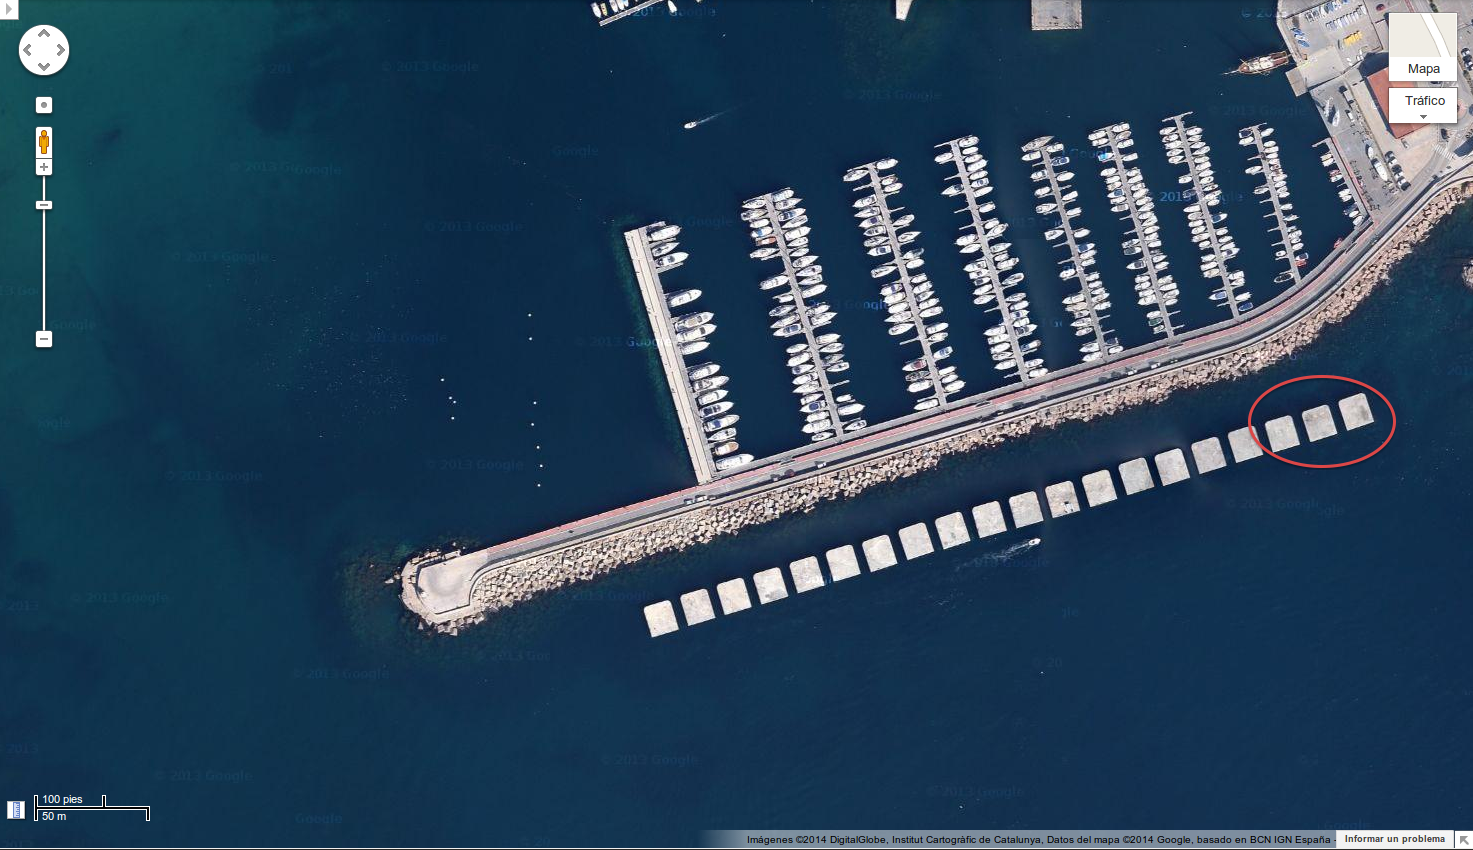
\includegraphics[width=.70\linewidth]{BreakwaterStructureSatelliteView}}
     \\%\quad
    \subfloat[]
    {\label{fig:BreakwaterStructureInternal}
    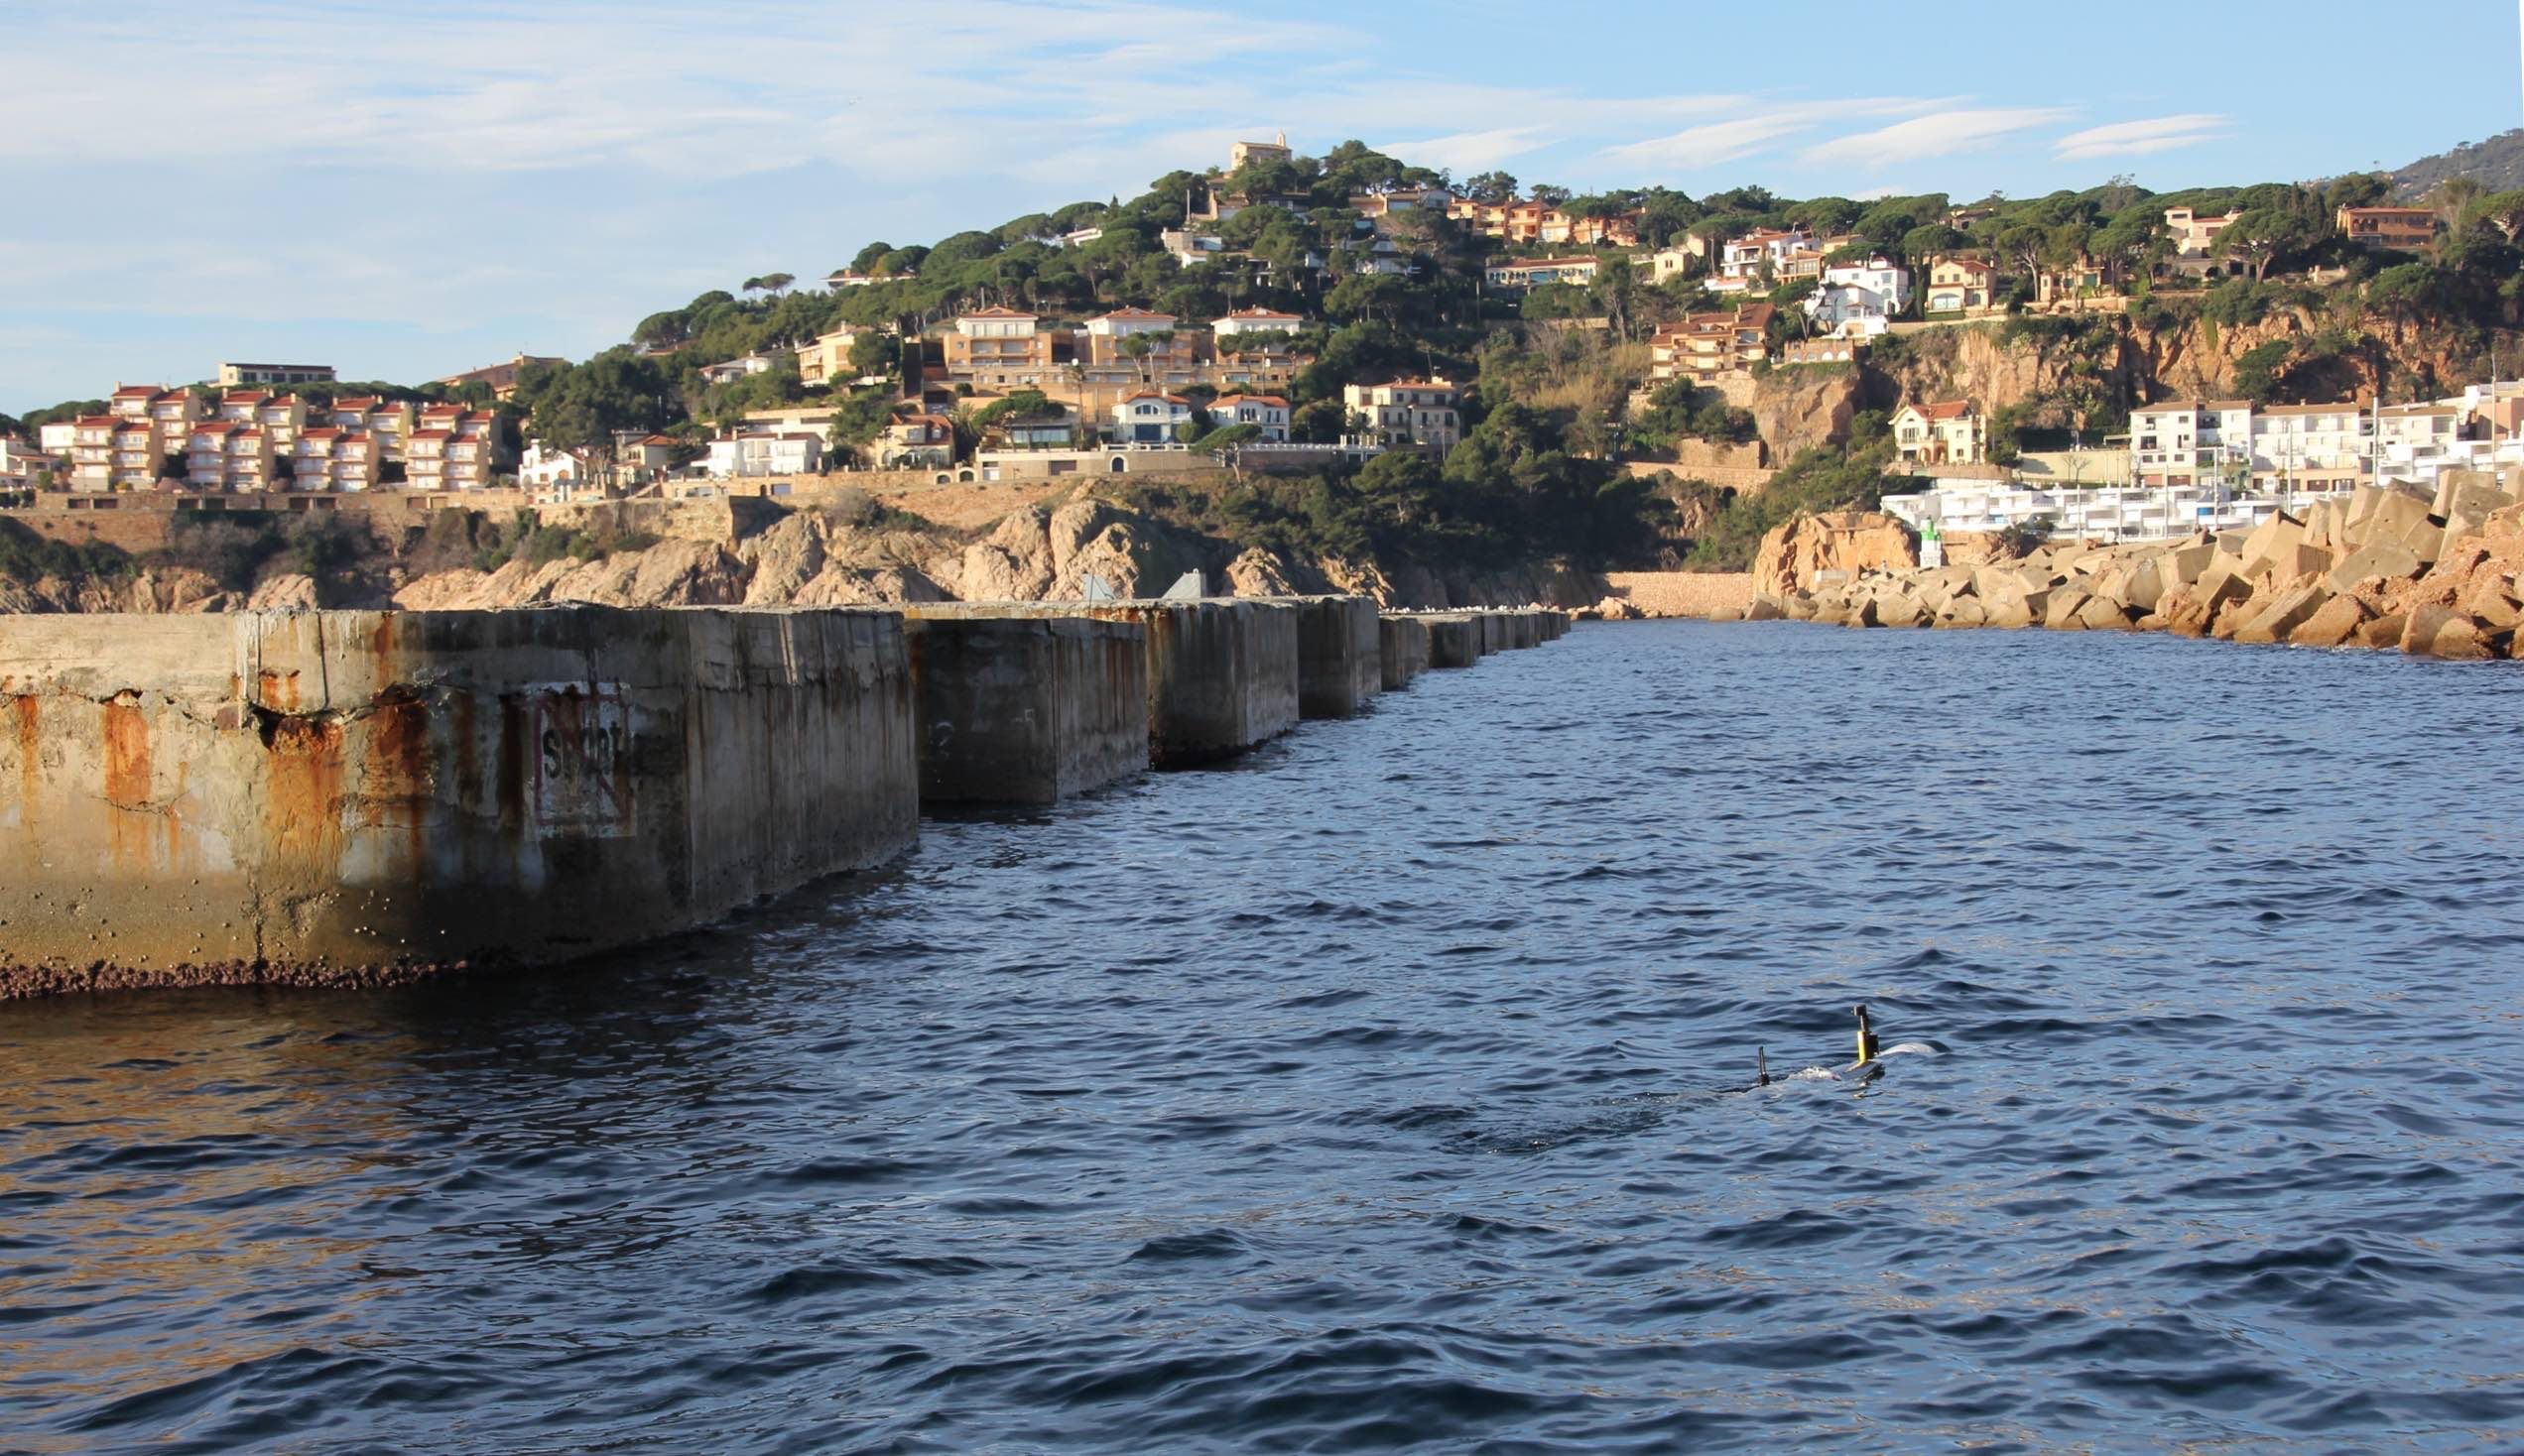
\includegraphics[width=.45\linewidth]{BreakwaterStructureInternal}} \quad
    \subfloat[]
    {\label{fig:BreakwaterStructureUWsim}
    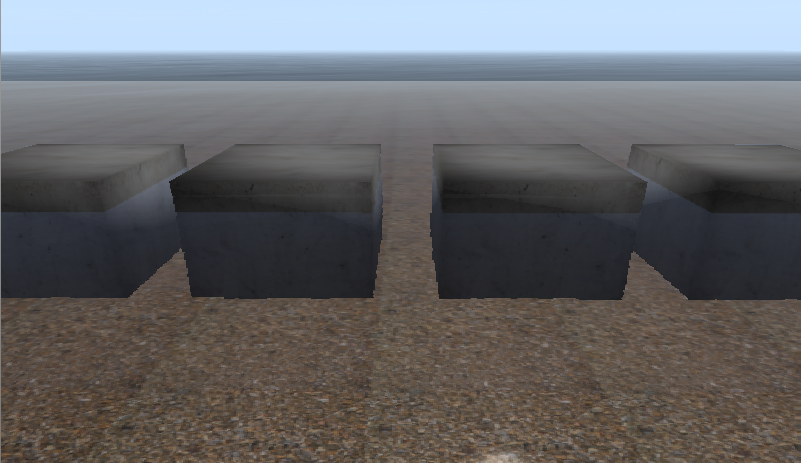
\includegraphics[width=.45\linewidth]{BreakwaterStructureUWsim}}
\caption[Test scenario of an artificial marine structure.]
{Test scenario of an artificial marine structure. 
\protect \subref{fig:SantFeliuPort} Harbor of Sant Feliu de Gu\'ixols in
Catalonia (Spain), where a breakwater structure composed of concrete blocks is
demarcated.
\protect \subref{fig:BreakwaterStructureInternal} Close proximity view of the
concrete blocks. \protect \subref{fig:BreakwaterStructureUWsim} Virtual
environment for simulations over \ac{UWSim}.}
\label{fig:BreakwaterStructure}
\end{figure}

As mentioned in previous chapters, an Octomap of the area can be used for
collision-checking purposes. Assuming the environment as explored, the Octomap
could be either one built from real data (see
Fig.~\ref{fig:ConcreteBlocksOctomap}) or one synthetically created (see
Fig.~\ref{fig:S2PlannOffBlocksRRTstarGeom3D}). Then, a collision-free, feasible
and safe path could be calculated over such a known map. Simulations of
this kind, \ie using an existing map, were presented in
Chapters~\ref{ch:motion_constratins}~and~\ref{ch:planning_3D}. However, before
conducting any real-world autonomous mission, the Sparus~II \ac{AUV} was
teleoperated at surface while traversing the concrete blocks. This allowed to
verify the map consistency with respect to the GPS data (see
Fig.~\ref{fig:S2TeleopConcrBlocks}).

\begin{figure}[htbp]
\myfloatalign
% 	\subfloat[]
%     {\label{fig:S2BetweenConcrBlocks}
%     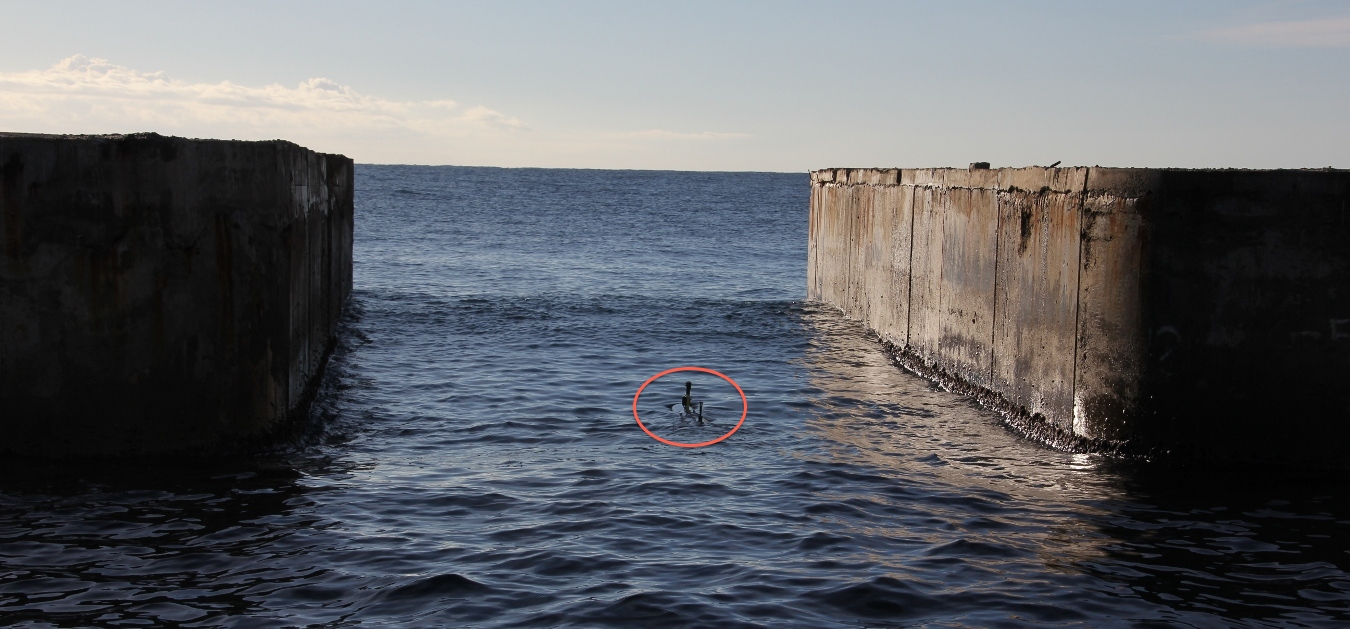
\includegraphics[width=.45\linewidth]{S2BetweenConcrBlocks}}\\%\quad
%     \subfloat[Satellite view. Image credit: Map data \copyright 2017 Google.]
%     {
    \label{fig:BreakwaterStructureGPSError}
     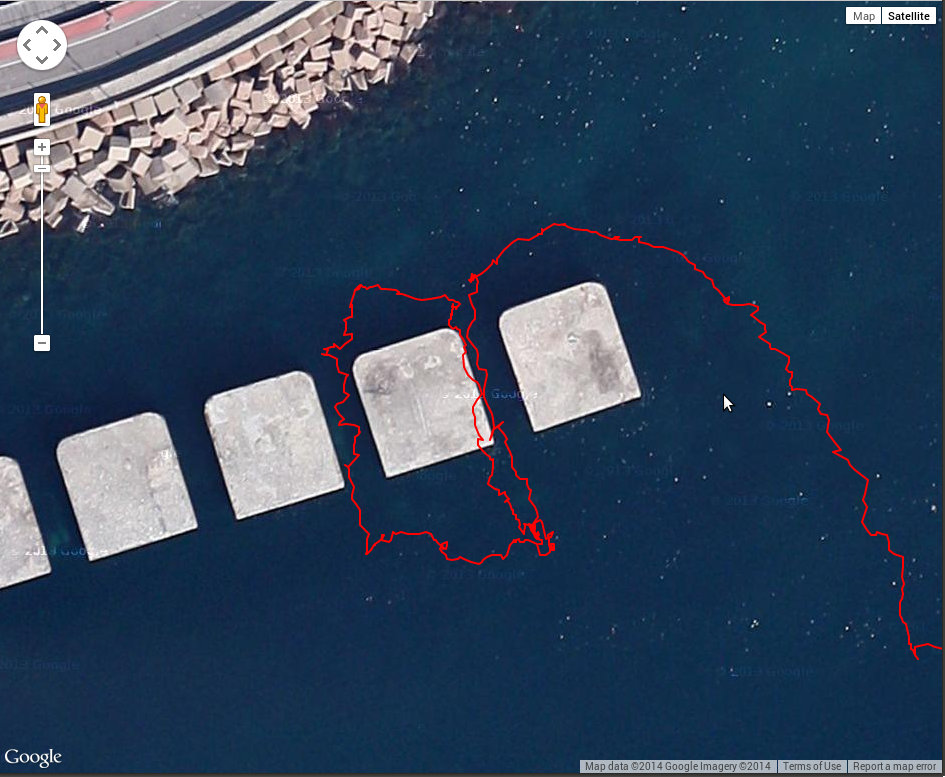
\includegraphics[width=.55\linewidth]{BreakwaterStructureGPSError}
%      }
\caption[Sparus~II AUV is teleoperated at surface in the breakwater structure
scenario.] 
{Sparus~II AUV was teleoperated at surface in the breakwater structure scenario.
% \protect \subref{fig:S2BetweenConcrBlocks} The vehicle, demarcated in red,
% moves between two concrete blocks. \protect
% \subref{fig:BreakwaterStructureGPSError} 
Although the Sparus~II did not collide
during the teleoperated mission, GPS data (in red) shows a vehicle trajectory
under collision with and even over the concrete blocks. Satellite view. Image
credit: Map data \copyright 2017 Google.}
\label{fig:S2TeleopConcrBlocks}
\end{figure}

Figure~\ref{fig:S2TeleopConcrBlocks} highlights one of the main limitations of
assuming the environment as previously known and mapped. Even if the \ac{AUV} is
teleoperated at surface, which allows to continuously obtain GPS fixes, there is
an error associated with the GPS that can range from one to two meters. This
magnitude of error is especially critical when navigating in narrow passages,
such as the four-meter gaps between the concrete blocks. Furthermore, if the
vehicle submerges, the position estimation error will also accumulate the
navigation drift associated with the \acf{DR} system. 

An alternative to conduct the intended mission could be the use of an \ac{USBL}
system, which would contribute to minimize the navigation error. Nonetheless,
this option requires a surface vessel that follows the \ac{AUV} along the
mission, something that is not feasible in this scenario. Considering all this,
an alternative approach is to use the framework proposed in this thesis.

As explained before, the framework requires that the vehicle is equipped with
exteroceptive sensors. These sensors allow detecting the surroundings to create
a map online. For this scenario, a set of four echosounders and one
mechanical-scanning imaging sonar were located within the vehicle payload
(front) area, all of them pointing in the horizontal plane (see
Fig.~\ref{fig:S2EchosMicronPayloadConf}). Three of the echosounders were
separated by $45^o$, with the central one looking forward and parallel to the
vehicle's direction of motion, while the fourth one was perpendicular to the
central one (see Fig.~\ref{fig:S2PayloadEchosMicron}). As for the imagining
sonar, it was setup to cover a scan sector in the vehicle's direction of motion
(see Fig.~\ref{fig:S2PayloadDirEchos}). Since both sensors cover the horizontal
plane, missions with this configuration were executed at a constant depth. For
more details about the complete Sparus~II's hardware configuration, the
interested reader is referred to Appendix~\ref{appx:exp_platform}.


\begin{figure}[htbp]
\myfloatalign
	\subfloat[]
    {\label{fig:S2PayloadEchosMicron}
     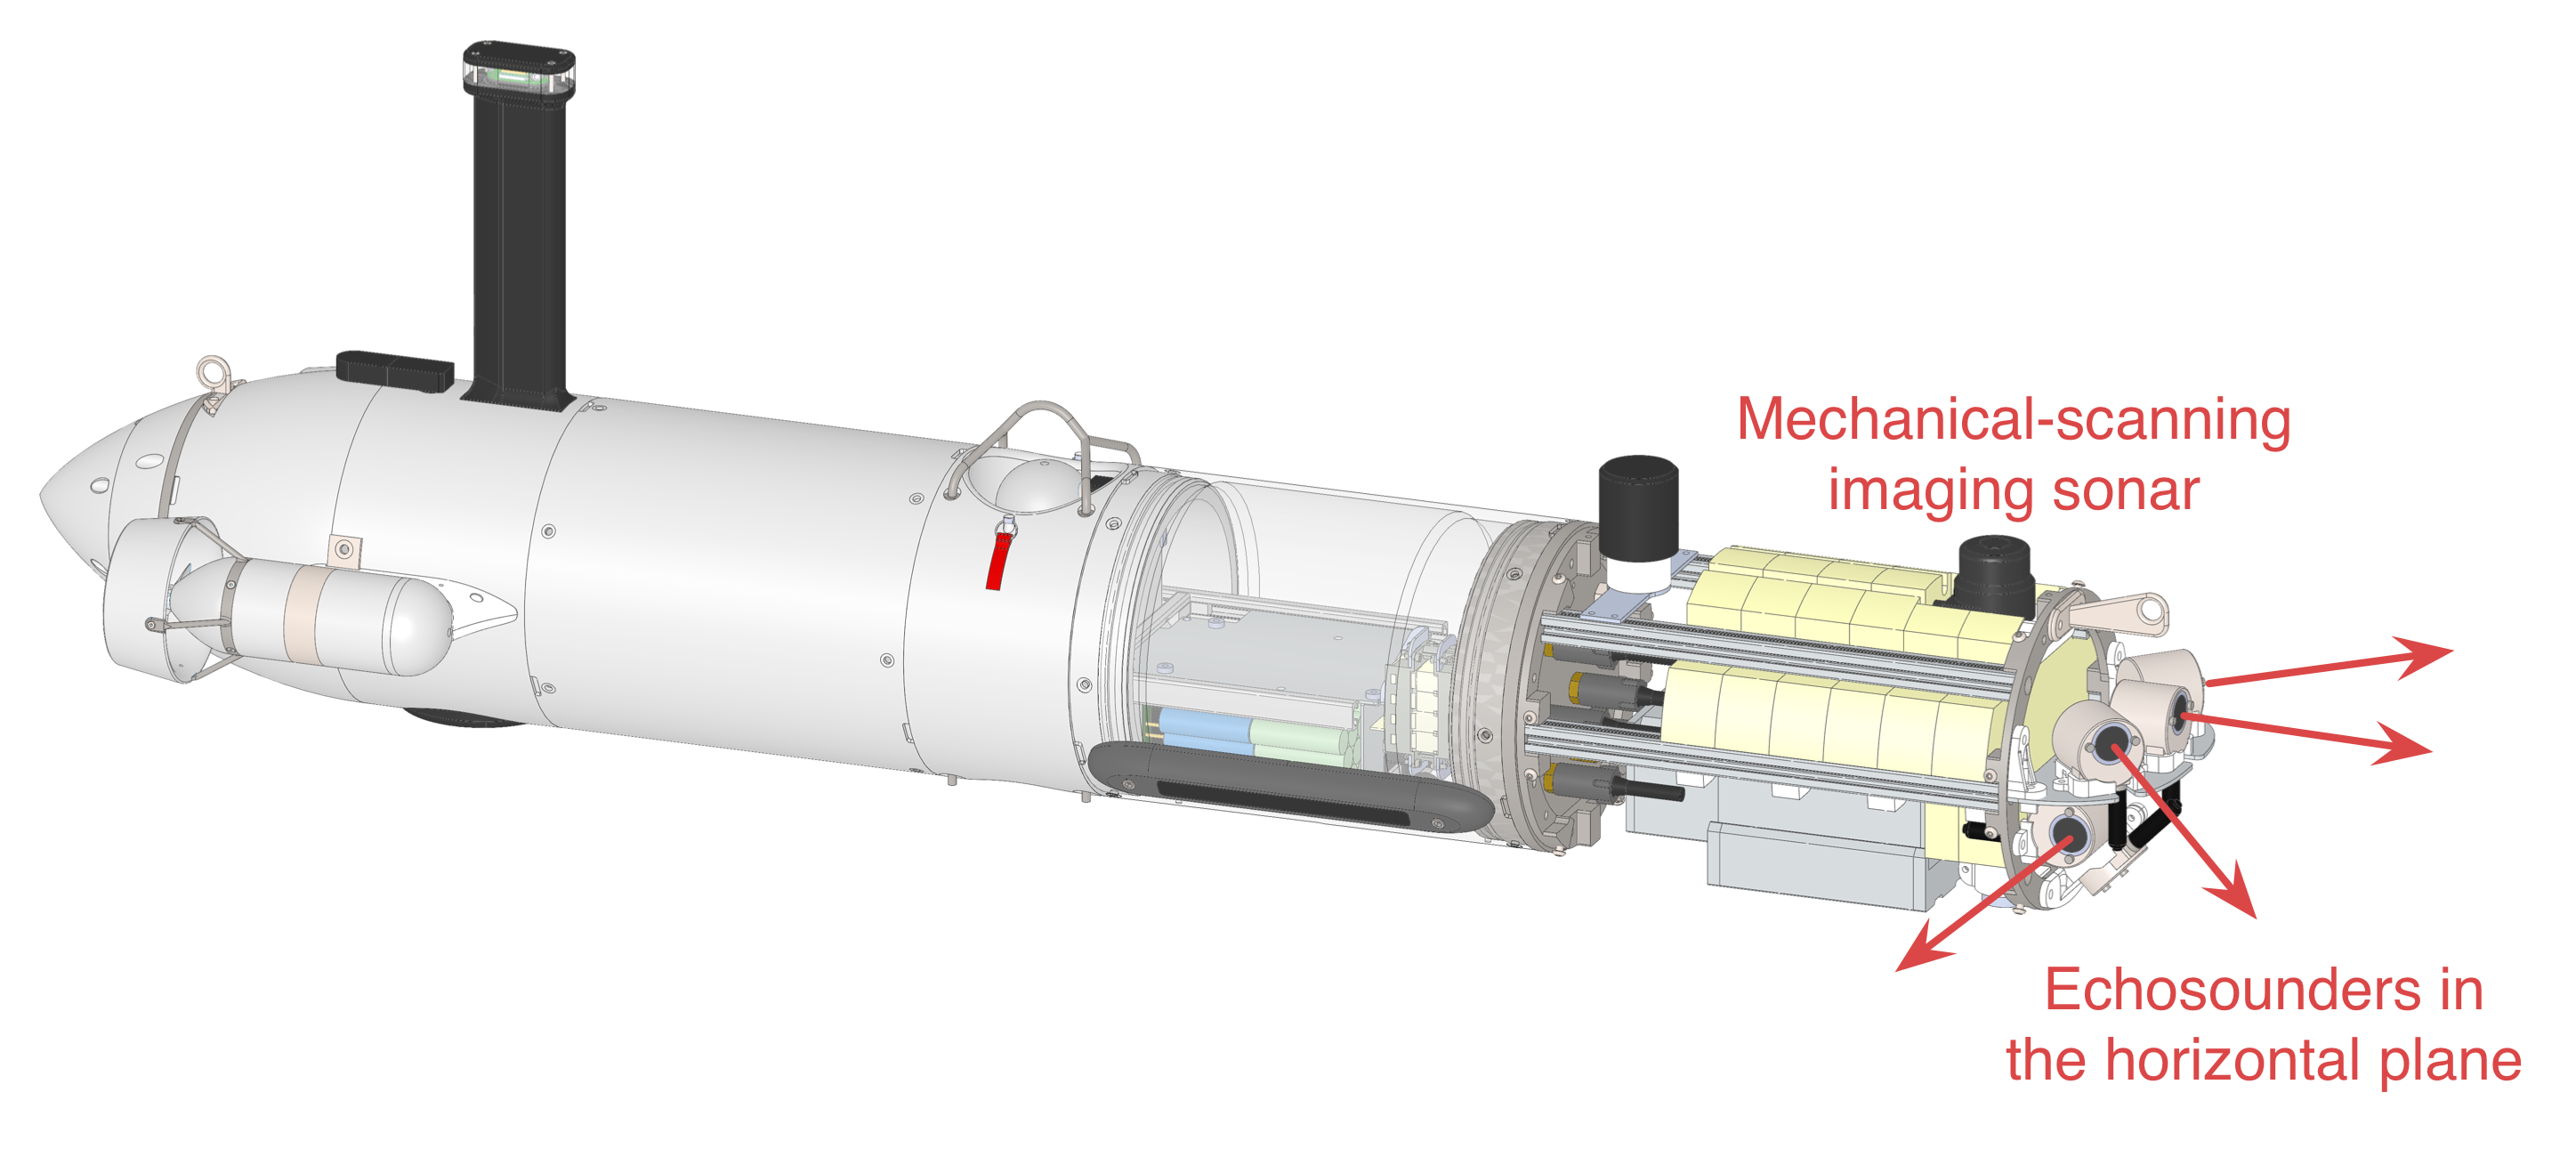
\includegraphics[width=.65\linewidth]{S2PayloadEchosMicron}}\\%\quad
	\subfloat[]
    {\label{fig:S2PayloadDirEchos}
    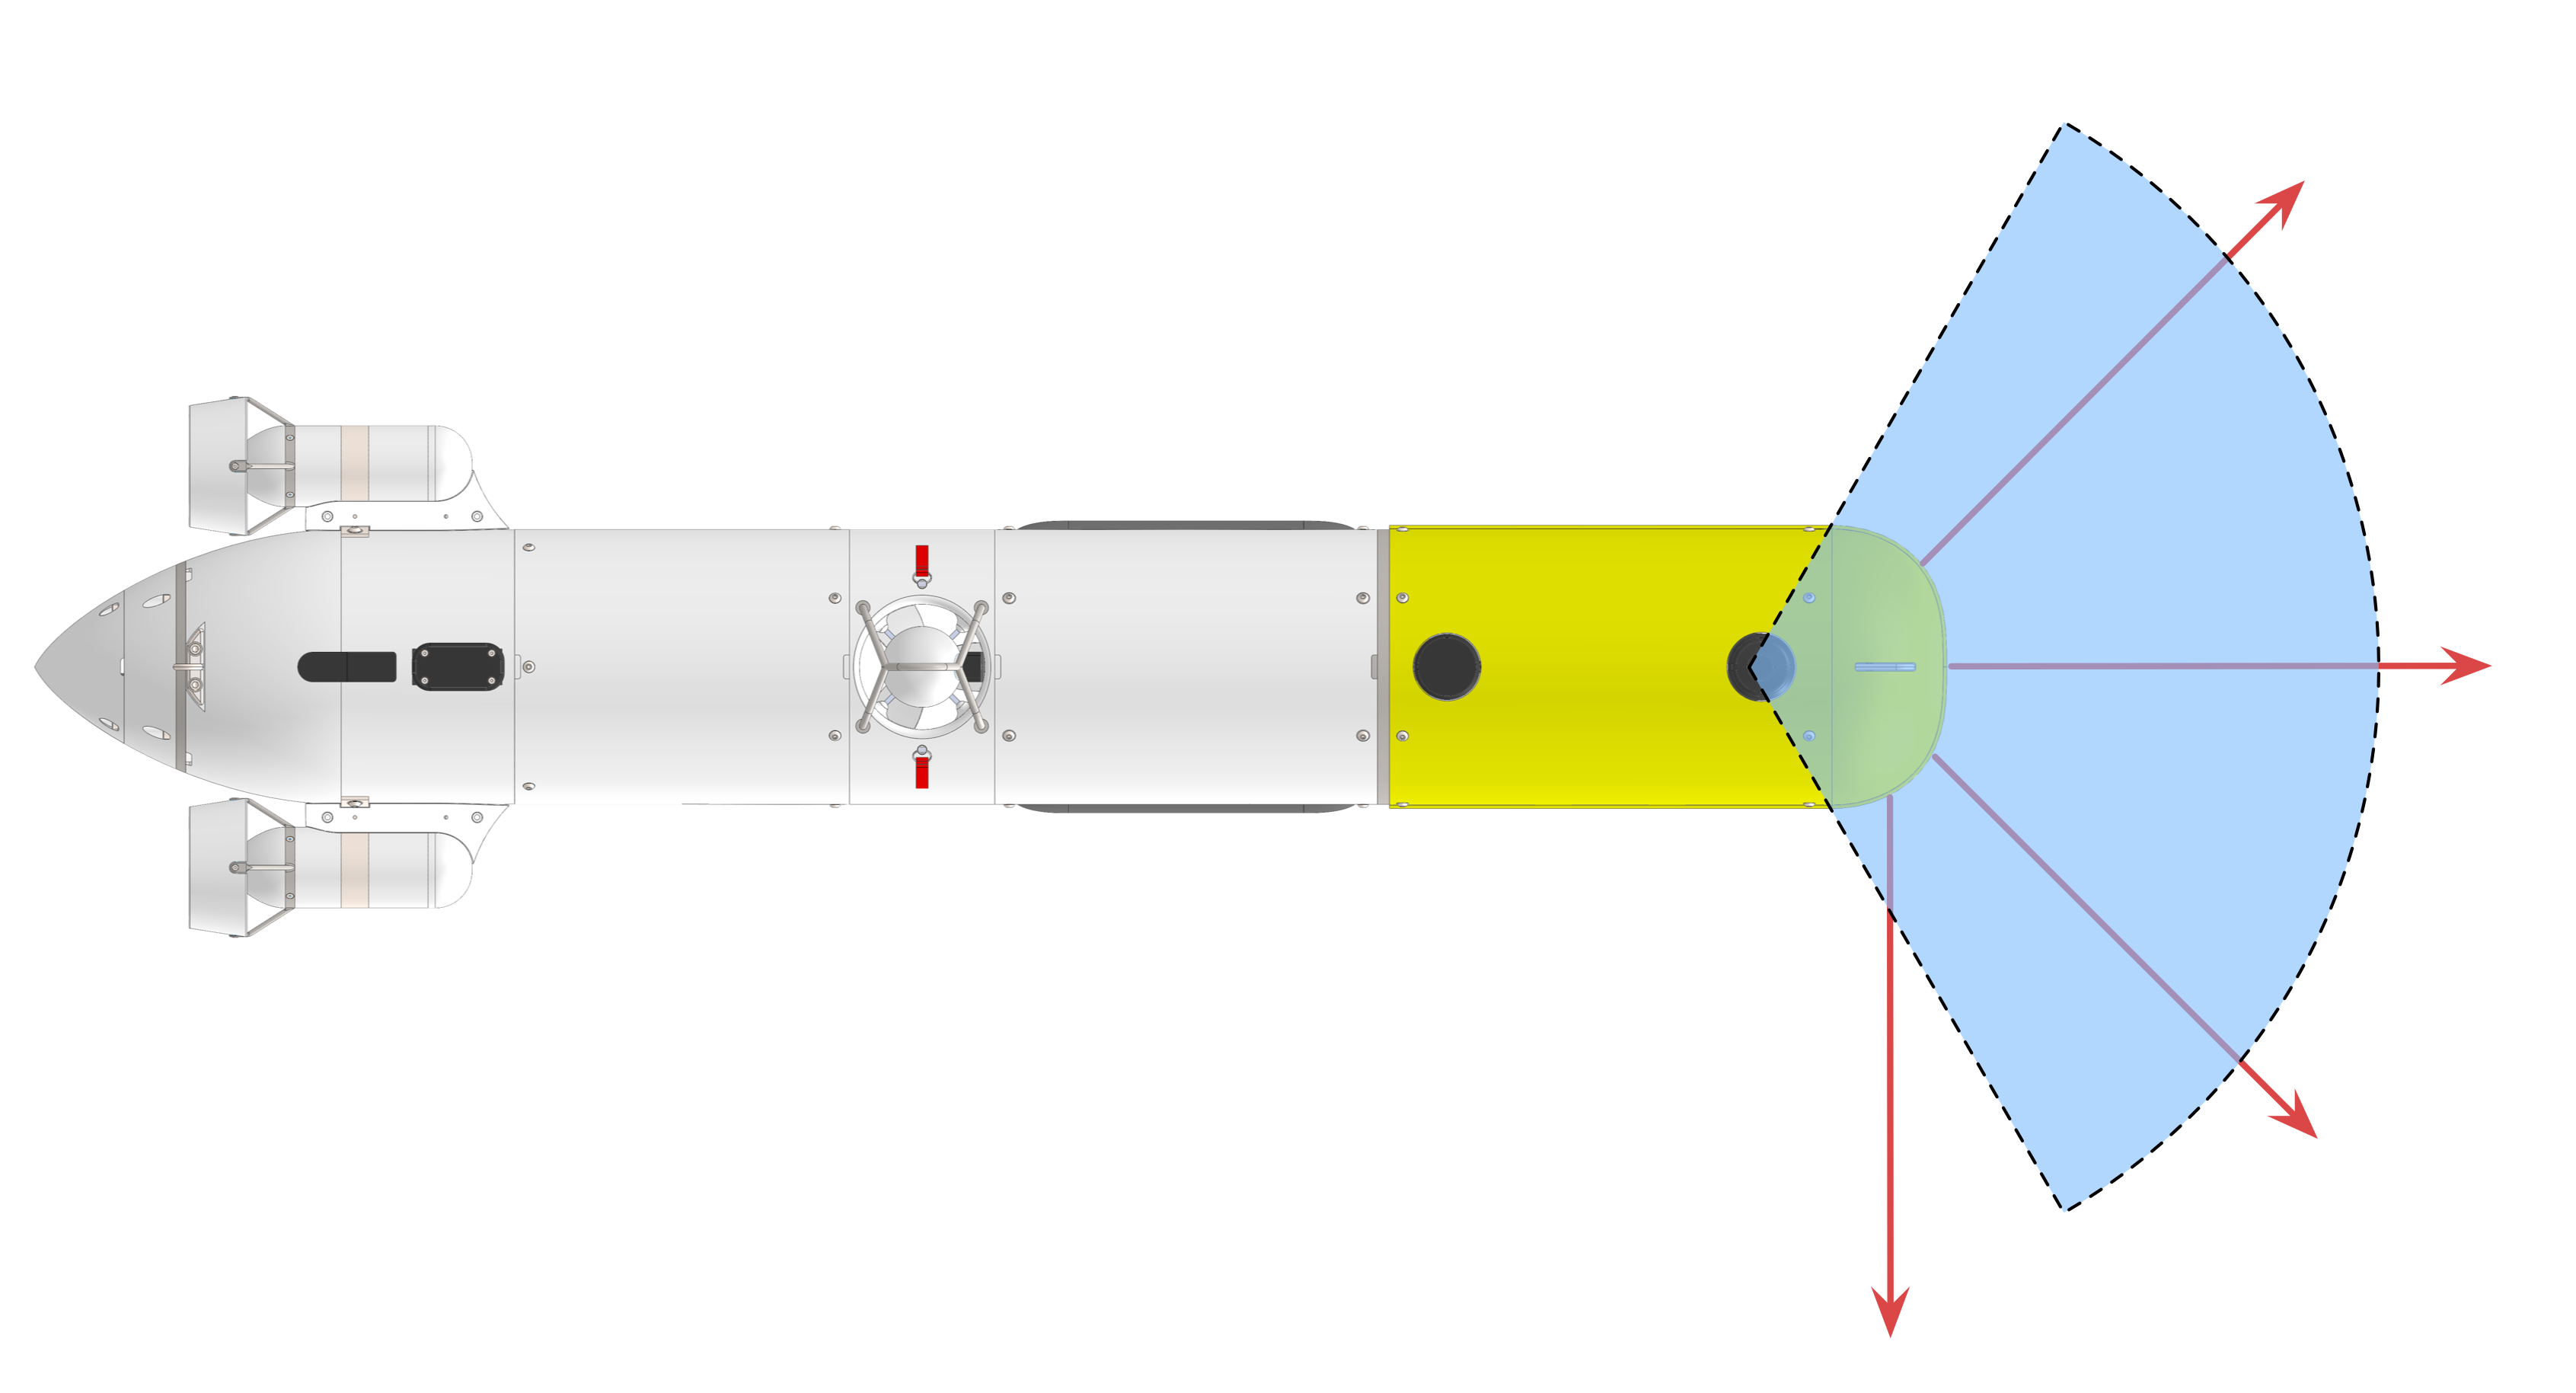
\includegraphics[width=.65\linewidth]{S2PayloadDirEchos}}
\caption[Exteroceptive sensors configuration for the Sparus~II AUV to
conduct autonomous missions in the breakwater structure.] 
{Exteroceptive sensors configuration for the Sparus~II AUV to
conduct autonomous missions in the breakwater structure.
\protect \subref{fig:S2PayloadEchosMicron} The vehicle was equipped with four
echosounders and one mechanical-scanning imaging sonar, all of them pointing in
the horizontal plane. \protect \subref{fig:S2PayloadDirEchos} Top view,
echosounders beams direction and imagining sonar scan sector.}
\label{fig:S2EchosMicronPayloadConf}
\end{figure}

During the first simulation and in-water trials conducted over this test
scenario, the Sparus~II \ac{AUV} only used the echosounders to perceive the
environment. Nevertheless, the four echosounders beams were insufficient to
rapidly establish the validity of the path along the direction of motion, which
triggered multiple replanning maneuvers. Although the vehicle was capable of
finding a solution path, it did required multiple attempts to complete one
full successful mission. Furthermore, this limitation generated unexpected and
non-desired trajectories. An example of this was already presented in
Chapter~\ref{ch:plann_online}, Fig.~\ref{fig:RealWOnReplannRRTStar}.

In order to avoid the aforementioned situations, the Sparus~II used both the
echosounders and the mechanical-scanning imaging sonar to incrementally build
the map. For each beam position within the scan sector, the imaging sonar
provided an array of intensities. From these intensity values, those that were
over a specified threshold represented the obstacles detected. Once those values
had been identified, they were transformed into ranges or distances to the
obstacles. However, since the imaging sonar has a vertical beamwidth of $35^o$,
the maximum range was limited to $10m$ to avoid false-positive detections from
the sea bottom. The echosounders, on the other hand, were setup with a maximum
range of $20m$, since they have a smaller beamwidth of $10^o$ (see
Appendix~\ref{appx:exp_platform}).

This payload configuration was used in different sea trials, and allowed the
vehicle to traverse the breakwater structure with great repeatability. To prove
this latter, the Sparus~II conducted missions that included multiple and
successive start-to-goal queries. Figure~\ref{fig:S2ConcrBlocksMultS2G} depicts
one of these missions. For safety reasons, the vehicle was connected to surface
with a wireless access point buoy that allowed us to monitor the mission and
abort it in case of detecting an unexpected behavior (see
Fig.~\ref{fig:S2BetweenConcrBlocksAutonomous}). For this mission, the
Sparus~II navigated with a constant surge speed $u=0.5m/s$, a maximum turning
rate $r_{max}=0.3rad/s$, and at a constant depth of $2m$. 

The mission was composed of three different and consecutive start-to-goal
queries, and assumed the environment as unexplored. Both the \ac{NED} reference
frame origin and the different goals coordinates when obtained from Google Maps
\copyright~2017. For the first query, the vehicle was initially in the inner
area of the breakwater structure, and the goal was a coordinate in the outer
area. Hence, the only possible solution path required the \ac{AUV}
to navigate through one of the four-meter gaps (see
Fig.~\ref{fig:S2BlocksMultS2GQ1}). The second query was set back in the inner
area but in a different coordinate, thus requiring to move through to one of the
gaps once again (see Fig.~\ref{fig:S2BlocksMultS2GQ2}). Likewise, the third and
last query was defined to conclude the mission in the outer area
(see Figs.~\ref{fig:S2BlocksMultS2GQ3},~\ref{fig:S2BlocksMultS2GQ4}).

\begin{figure}[htbp]
\myfloatalign
	\subfloat[]
    {\label{fig:S2BetweenConcrBlocksAutonomous}
     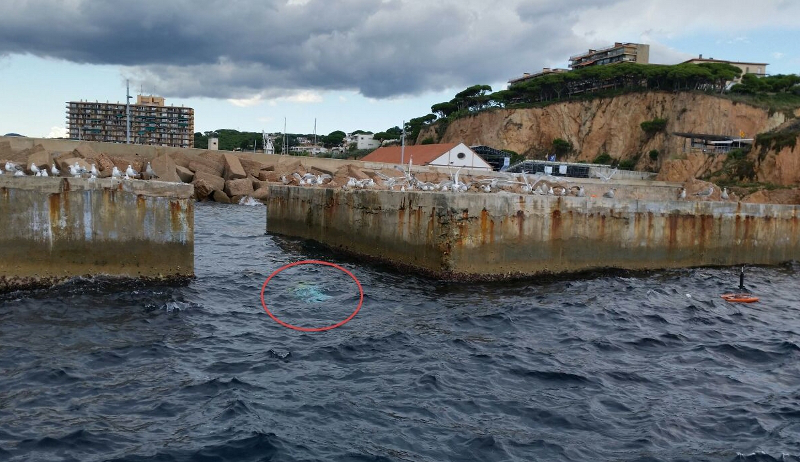
\includegraphics[width=.60\linewidth]{S2BetweenConcrBlocksAutonomous}}\\%\quad
	\subfloat[]
    {\label{fig:S2BlocksMultS2GQ1}
    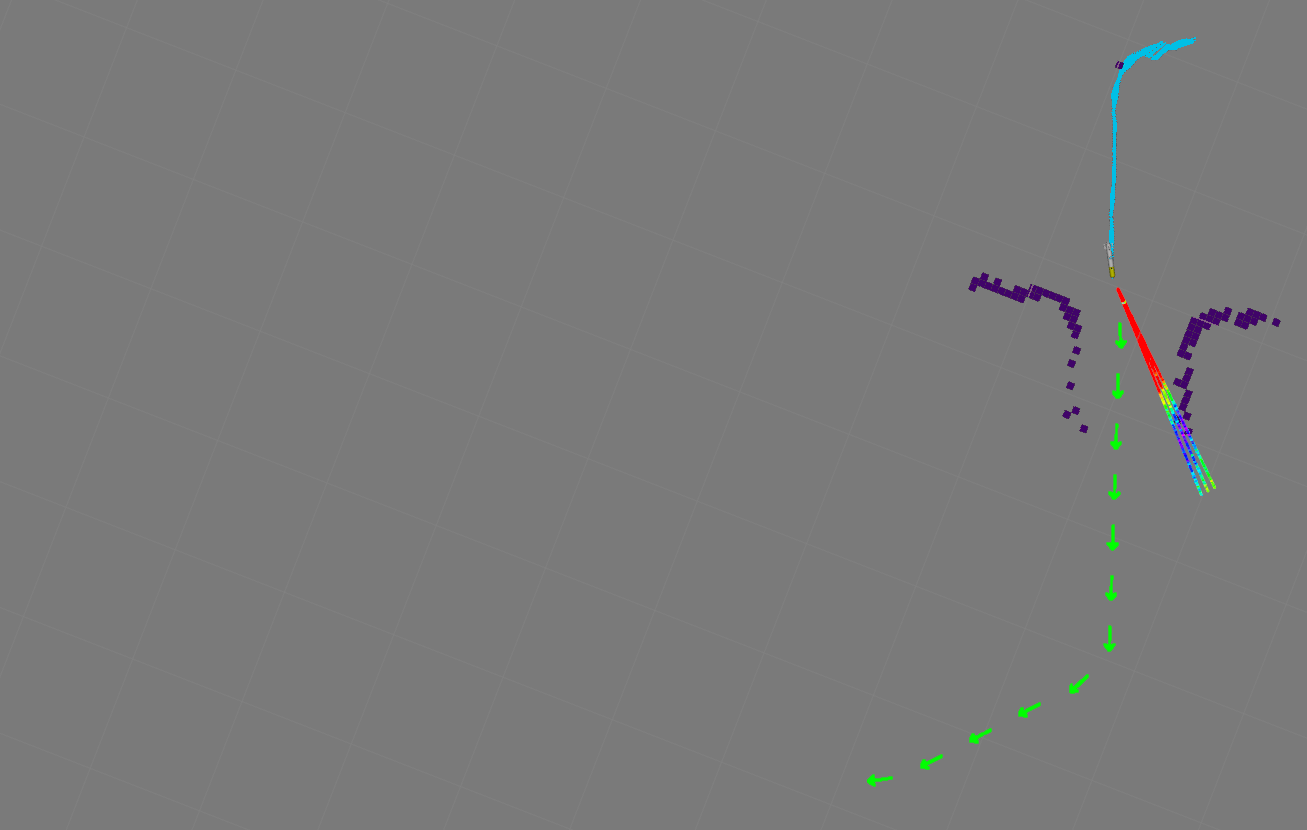
\includegraphics[width=.45\linewidth]{S2BlocksMultS2GQ1}}\quad
    \subfloat[]
    {\label{fig:S2BlocksMultS2GQ2}
    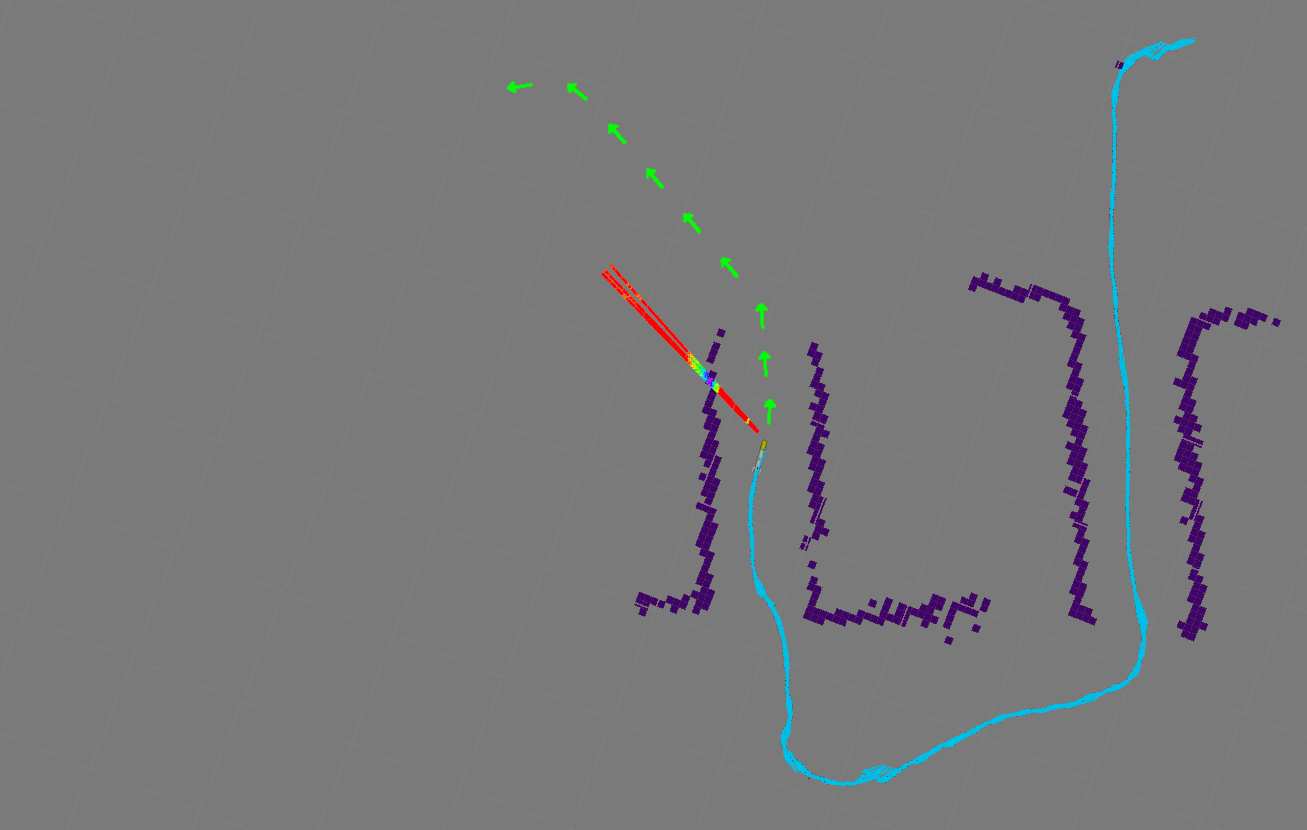
\includegraphics[width=.45\linewidth]{S2BlocksMultS2GQ2}}\\%\quad
	\subfloat[]
    {\label{fig:S2BlocksMultS2GQ3}
    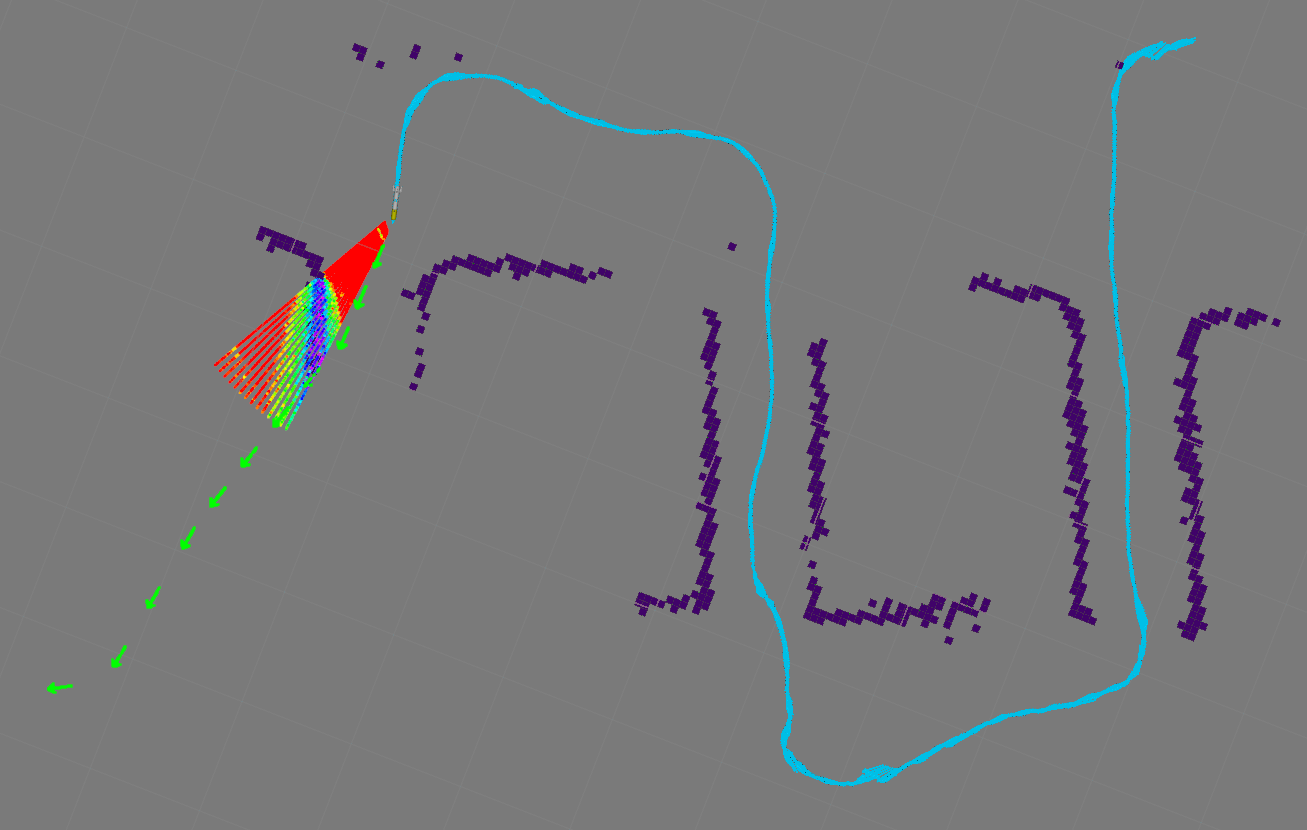
\includegraphics[width=.45\linewidth]{S2BlocksMultS2GQ3}}\quad
    \subfloat[]
    {\label{fig:S2BlocksMultS2GQ4}
    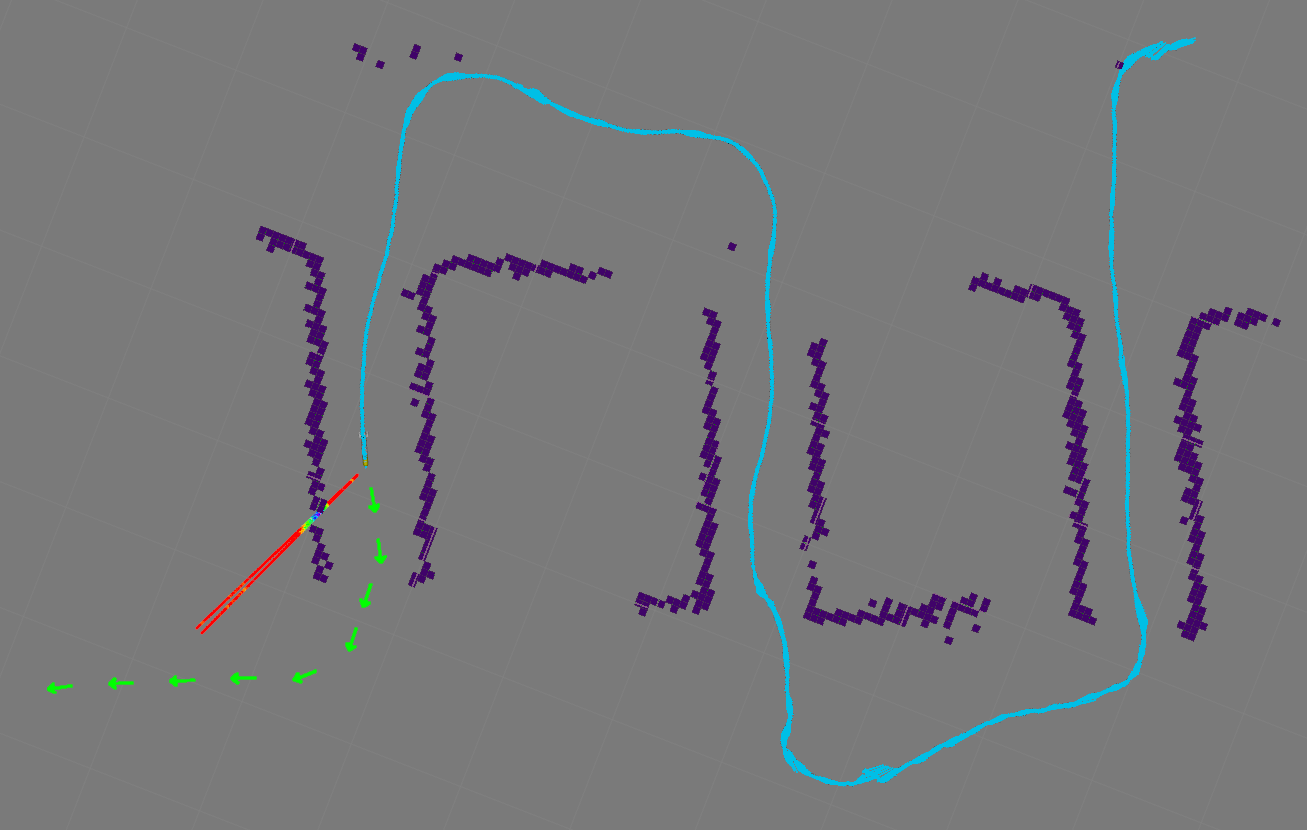
\includegraphics[width=.45\linewidth]{S2BlocksMultS2GQ3_}}\\%\quad
    \subfloat[]
    {\label{fig:S2BlocksMultS2GGoogleMaps}
    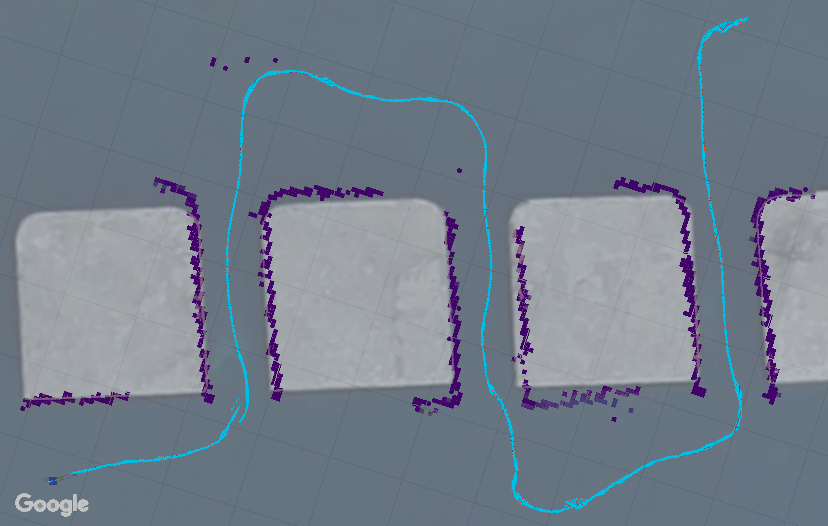
\includegraphics[width=.45\linewidth]{S2BlocksMultS2GGoogleMaps}}
\caption[The Sparus II AUV using the path/motion planning framework to navigate
through a breakwater structure without a preliminary map of the surroundings.]
{The Sparus II \ac{AUV} used the path/motion planning
framework to navigate through a breakwater structure without a preliminary
map of the surroundings.
\protect \subref{fig:S2BetweenConcrBlocksAutonomous} The vehicle is submerged
and is moving autonomously amidst two concrete blocks.
\protect \subref{fig:S2BlocksMultS2GQ1}, \protect
\subref{fig:S2BlocksMultS2GQ2}, \protect \subref{fig:S2BlocksMultS2GQ3},
\protect \subref{fig:S2BlocksMultS2GQ4} The mission required traversing the
breakwater structure multiple times by solving successive start-to-goal
queries.
\protect \subref{fig:S2BlocksMultS2GGoogleMaps} The vehicle trajectory is drawn
in light blue, while the map built with the imaging sonar data is presented in
purple. This information is overlapped with a satellite image (Google Maps
\copyright~2017).}
\label{fig:S2ConcrBlocksMultS2G}
\end{figure}

Along the mission, the Sparus~II did not surface to obtain GPS fixes.
Figure~\ref{fig:S2BlocksMultS2GGoogleMaps} depicts the vehicle trajectory and
the Octomap built overlapped with a satellite imagine of the breakwater structure.
Although the Octomap is coherent with respect to the real-world structure, there
are some differences due to the accumulation of navigation error. Yet this did
not prevent the \ac{AUV} from completing successfully the mission.

To further discuss potential applications,
Figure~\ref{fig:Breakwater3DReconstruction} depicts a photo-realistic \ac{3D}
model of the area traveled by the Sparus~II during the mission presented above.
In this particular mission, the \ac{AUV} used a stereo optical camera, which
gathered additional data from the surroundings. Such information was used to
create a more detailed survey of the area after concluding the mission. Other
missions may include sensors to measure different variables of interest, such as
biological, chemical, as well as bathymetric information. For more details about
these \ac{3D} reconstructions, the interested reader is referred
to~\cite{Hernandez2016,Hernandez2016a}.

\begin{figure}[htbp]
\myfloatalign
	\subfloat[]
    {\label{fig:Breakwater3DReconstruction2}
    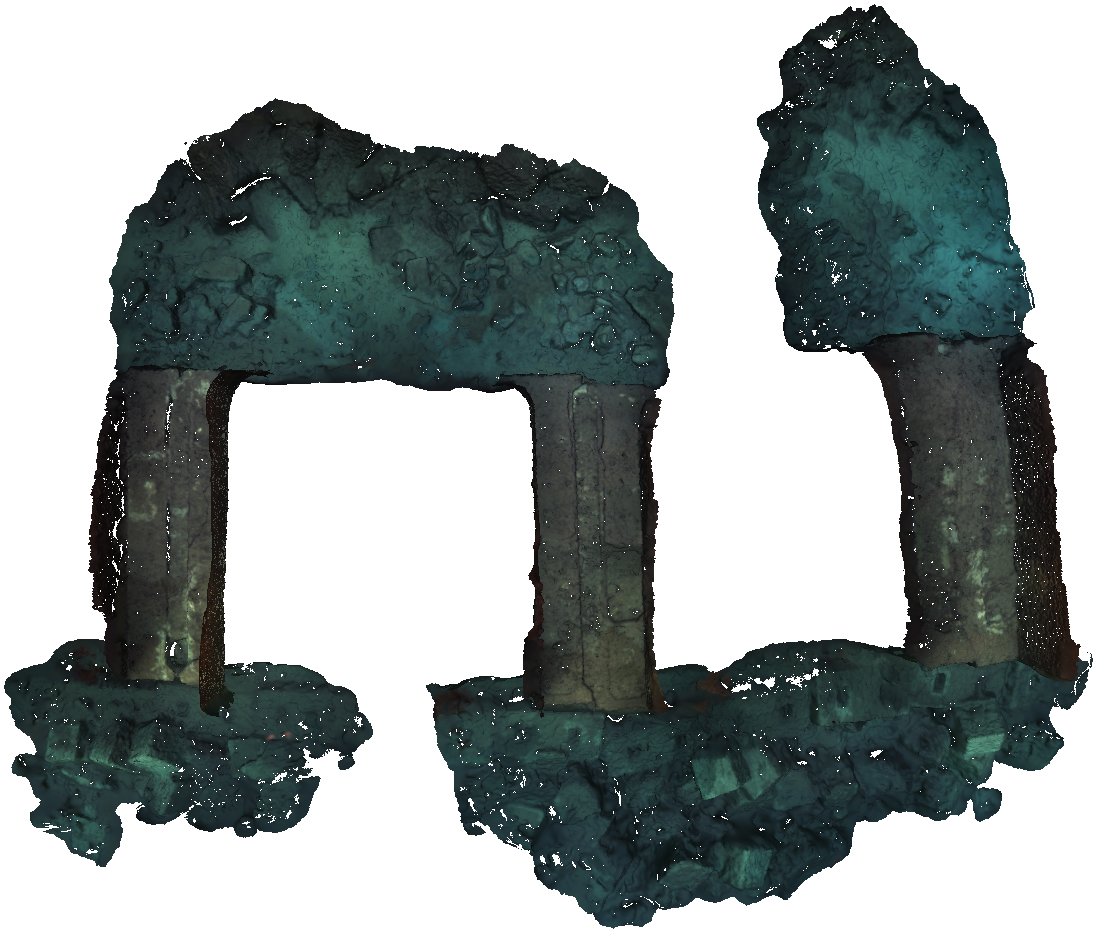
\includegraphics[width=.85\linewidth]{Breakwater3DReconstruction2}}\\
	\subfloat[]
    {\label{fig:Breakwater3DReconstruction3}
     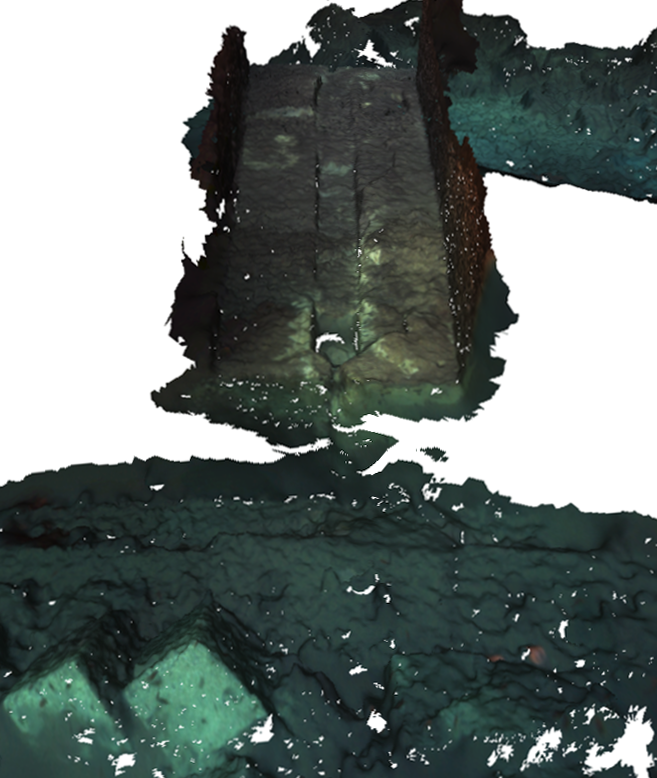
\includegraphics[width=.4\linewidth]{Breakwater3DReconstruction3}}\quad
	\subfloat[]
    {\label{fig:Breakwater3DReconstruction4}
    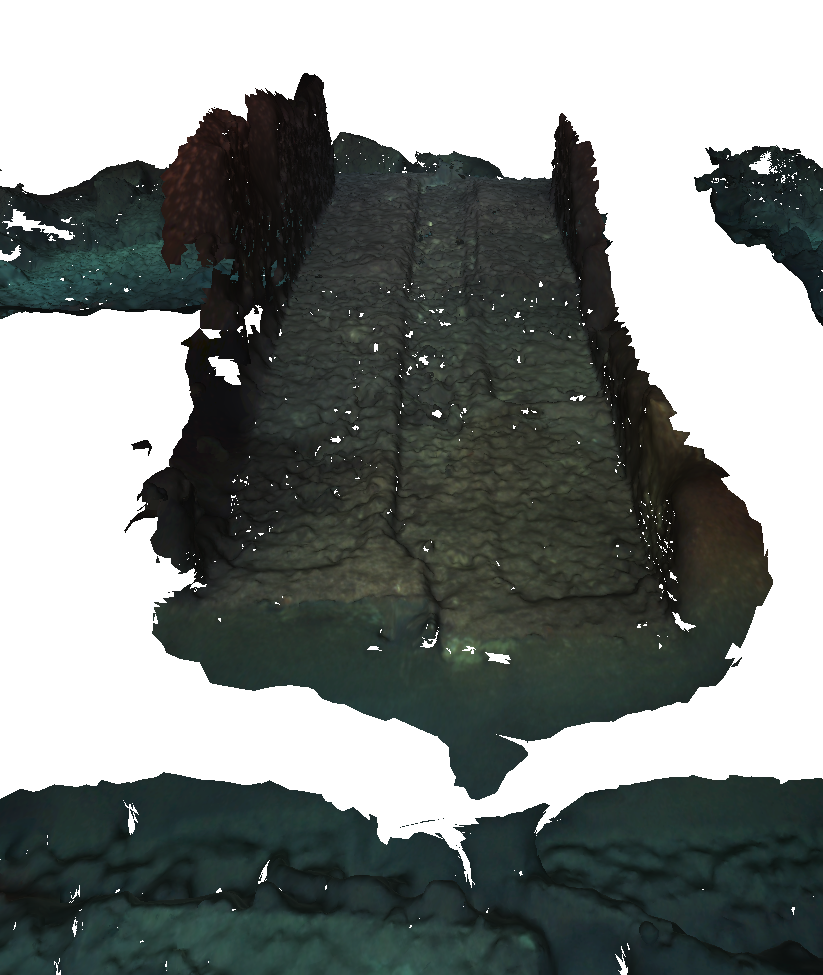
\includegraphics[width=.4\linewidth]{Breakwater3DReconstruction4}}
% 	\subfloat[]
%     {\label{fig:Breakwater3DReconstruction1}
%      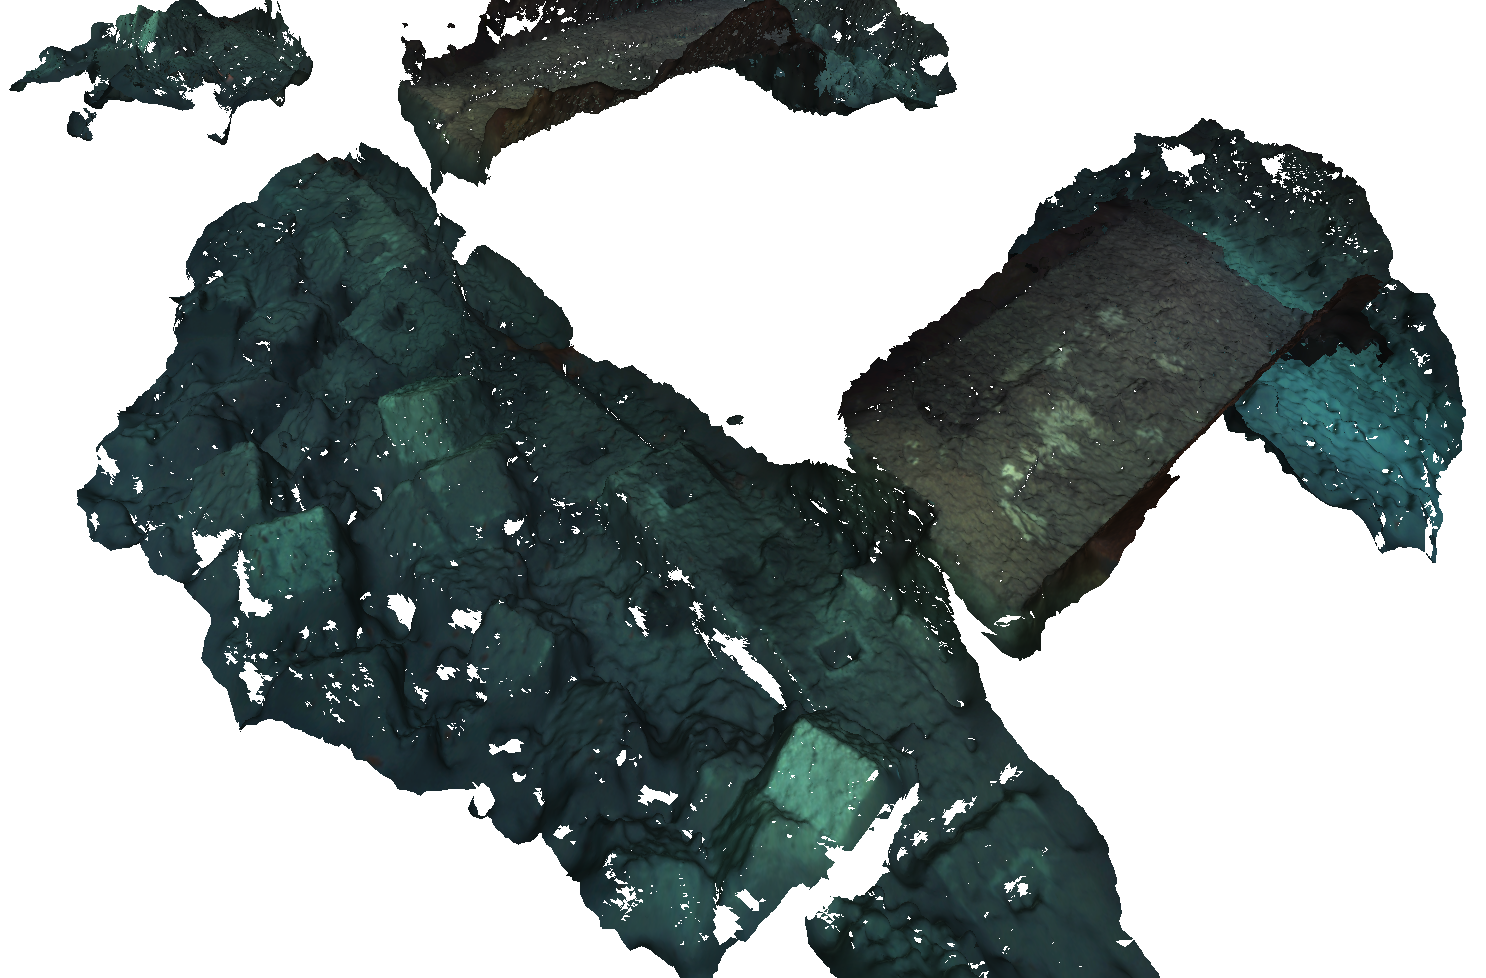
\includegraphics[width=.80\linewidth]{Breakwater3DReconstruction1}}\\%\quad
\caption[3D reconstruction built from images gathered along the autonomous
mission presented in Fig.~\ref{fig:S2ConcrBlocksMultS2G}.] 
{\protect \subref{fig:3Drecon_top} Top-down view of the textured 3D model built
with the images gathered along the mission shown in
Fig.~\ref{fig:S2ConcrBlocksMultS2G}.
\protect \subref{fig:Breakwater3DReconstruction3},\protect
\subref{fig:Breakwater3DReconstruction4} 3D views of the corridors or gaps
between the concrete blocks.}
\label{fig:Breakwater3DReconstruction}
\end{figure}

\section{Planning AUV Paths in Natural Marine Formations}

Although the mission in the breakwater structure represents a valid
application example, it is also true that the obstacles in it, \ie the concrete
blocks, have regular shapes. Their vertical walls, for instance, were correctly
detected by a mechanical-scanning imaging sonar, despite its great beamwidth.
Natural environments, on the other hand, present less regular and more
challenging scenarios. Therefore and in order to prove the proposed framework
under different conditions, the Sparus~II also conducted autonomous missions
over a real-world natural environment. The testing area is also located in Sant
Feliu de Gu\'ixols (Spain), and contains rocky formations that create an
underwater canyon (see Fig.~\ref{fig:RockyFormationCanyon}).


\begin{figure}[htbp]
\myfloatalign
    \subfloat[Satellite view. Image credit: Map data \copyright 2017 Google.]
    {\label{fig:RockyFormationCanyonSatelliteView}
     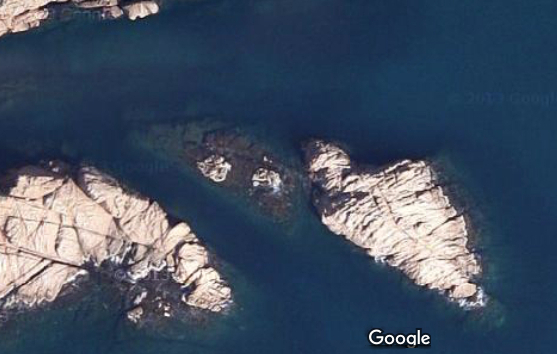
\includegraphics[width=.60\linewidth]{RockyFormationCanyonSatelliteView}}
     \\%\quad
    \subfloat[]
    {\label{fig:RockyFormationCanyonInner}
    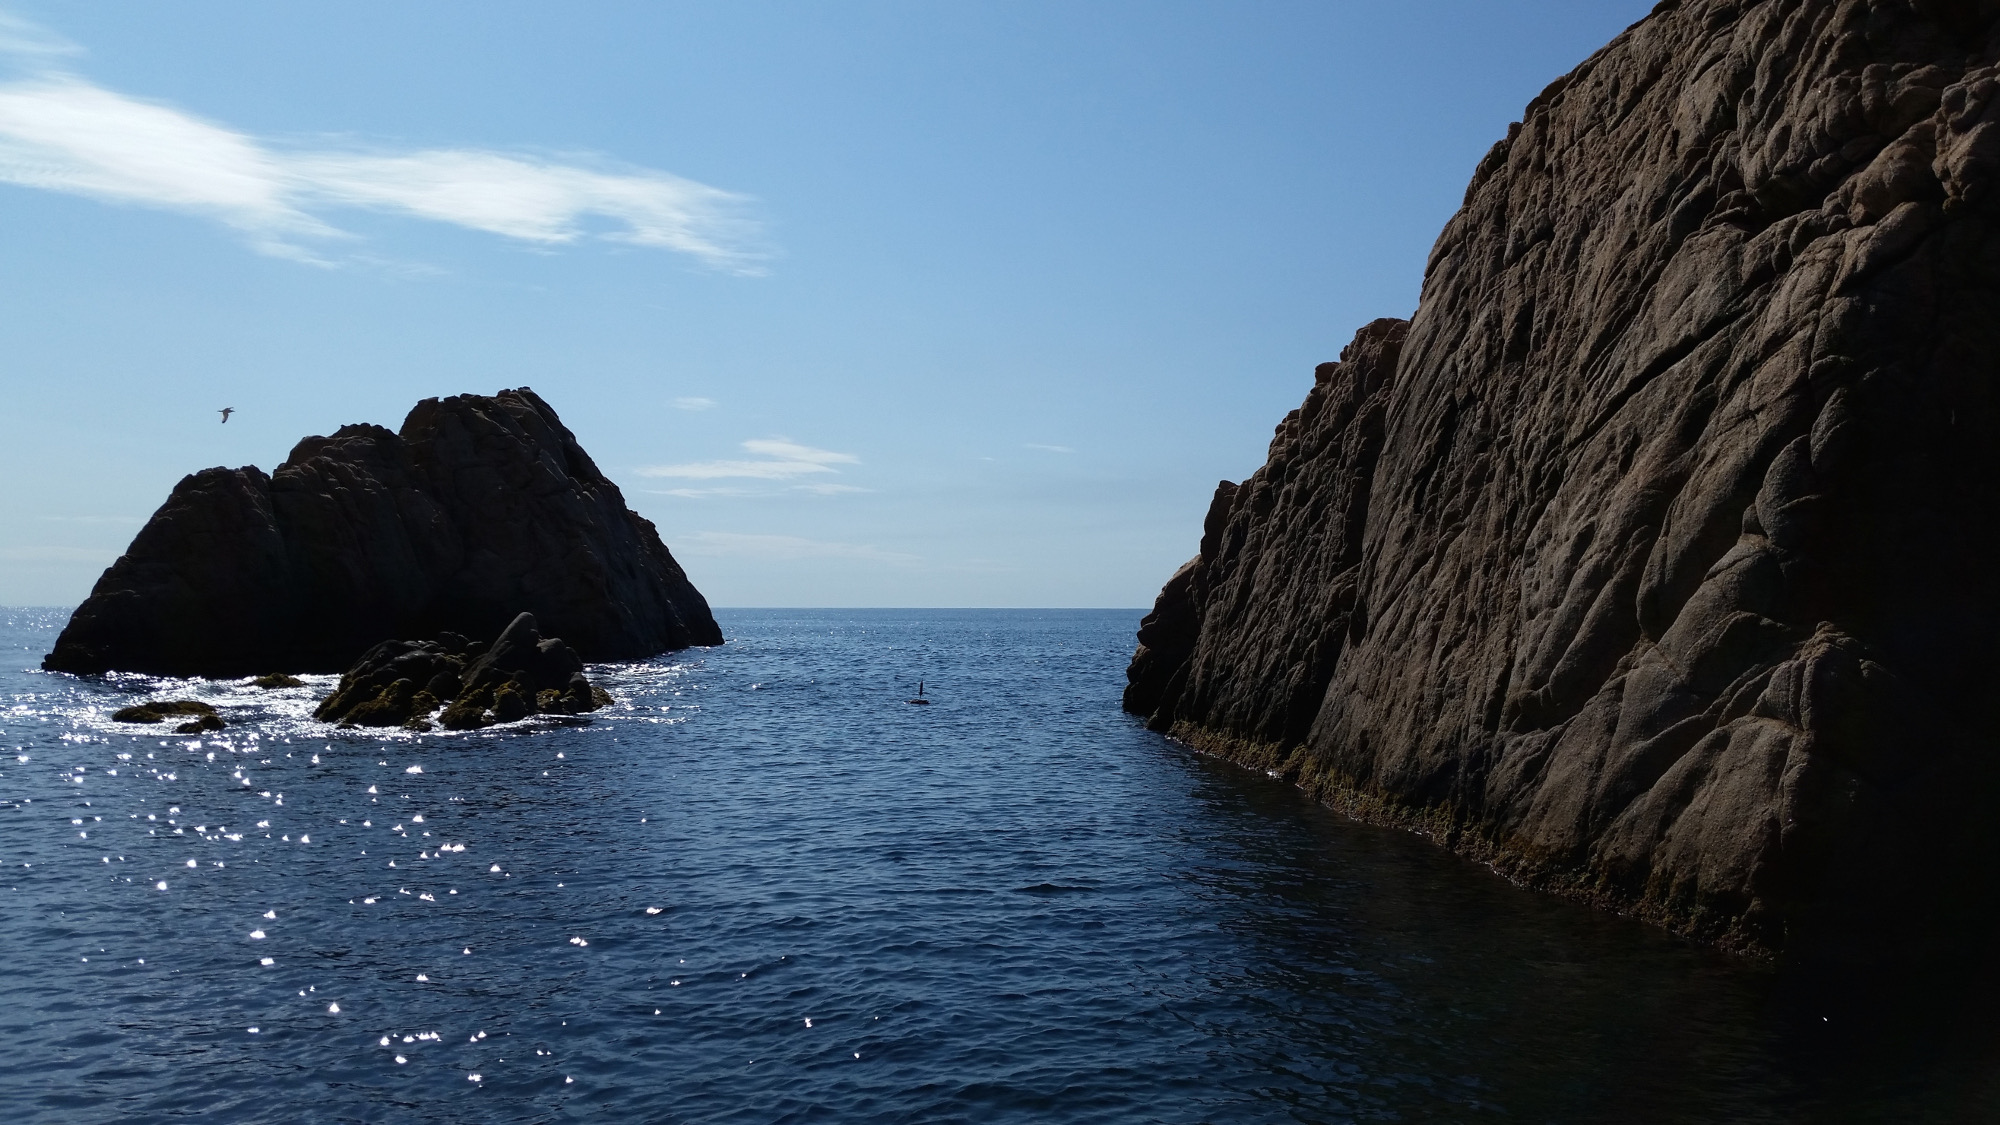
\includegraphics[width=.45\linewidth]{RockyFormationCanyonInner}} \quad
    \subfloat[]
    {\label{fig:RockyFormationCanyonOuter}
    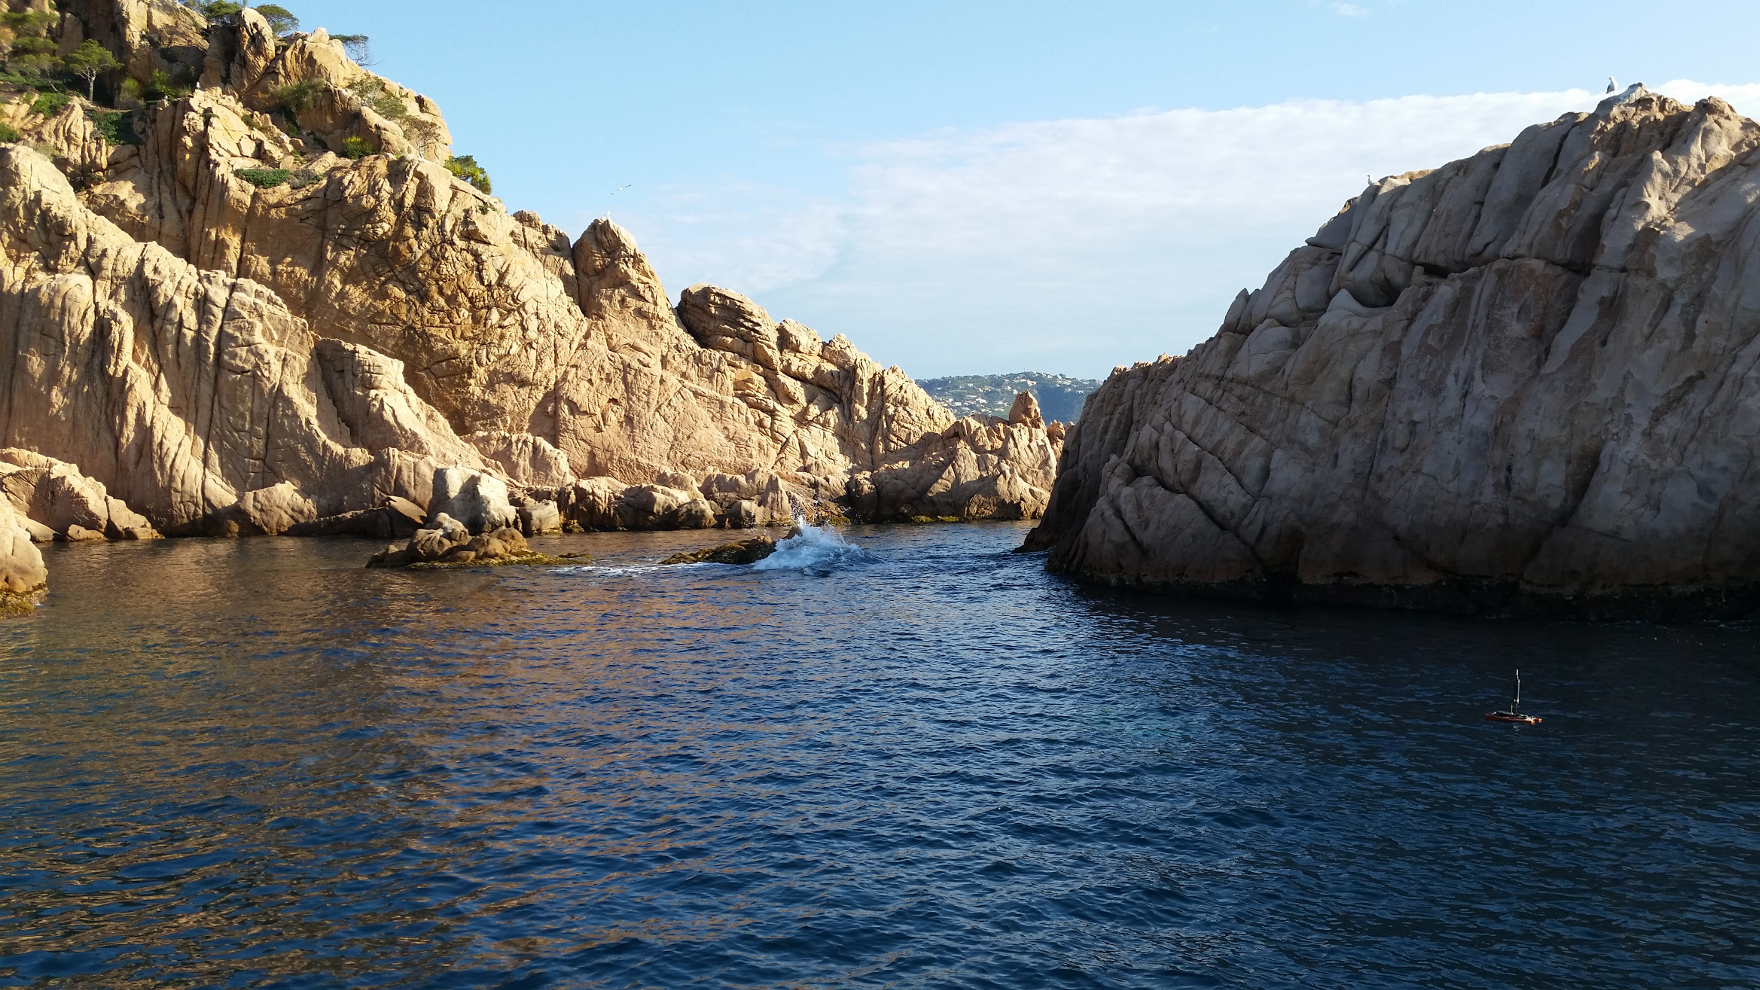
\includegraphics[width=.45\linewidth]{RockyFormationCanyonOuter}}
\caption[Test scenario of a natural marine formation.]
{The test scenario consists of rocky formations.
\protect \subref{fig:RockyFormationCanyonSatelliteView} They create an
underwater canyon that can be observed in the satellite image.
\protect \subref{fig:RockyFormationCanyonInner} From the inner area (\ie from
the coastline towards the open sea) the canyon can be clearly observed.
\protect \subref{fig:RockyFormationCanyonOuter} From the outer area the canyon
can be observed in the left.}
\label{fig:RockyFormationCanyon}
\end{figure}

For this scenario, the Sparus~II \ac{AUV} used a mechanic-scanning profiling
sonar, which has a smaller beamwidth of $1-2^o$ (see
Appendix~\ref{appx:exp_platform}). This sensor, which covered the horizontal
plane, permitted not only to perceive the obstacles shape with more accuracy,
but also to set a higher maximum range without being affected by false-positive
detections from the bottom. The \ac{AUV} was also equipped with a set of three
GoPro\texttrademark{} Hero 4 Black edition cameras. They were used to gather the
optical images required to create a \ac{3D} reconstruction of the surroundings.
The cameras were positioned systematically to ensure the highest possible
coverage, where two of them were placed in a downward configuration at an angle
of $20^o$, while the third camera was positioned forward looking at $40^o$ (see
Fig.~\ref{fig:S2ProfCamsPayloadConf}).

\begin{figure}[htbp]
\myfloatalign
	\subfloat[]
    {\label{fig:S2PayloadProfilerCameras}
     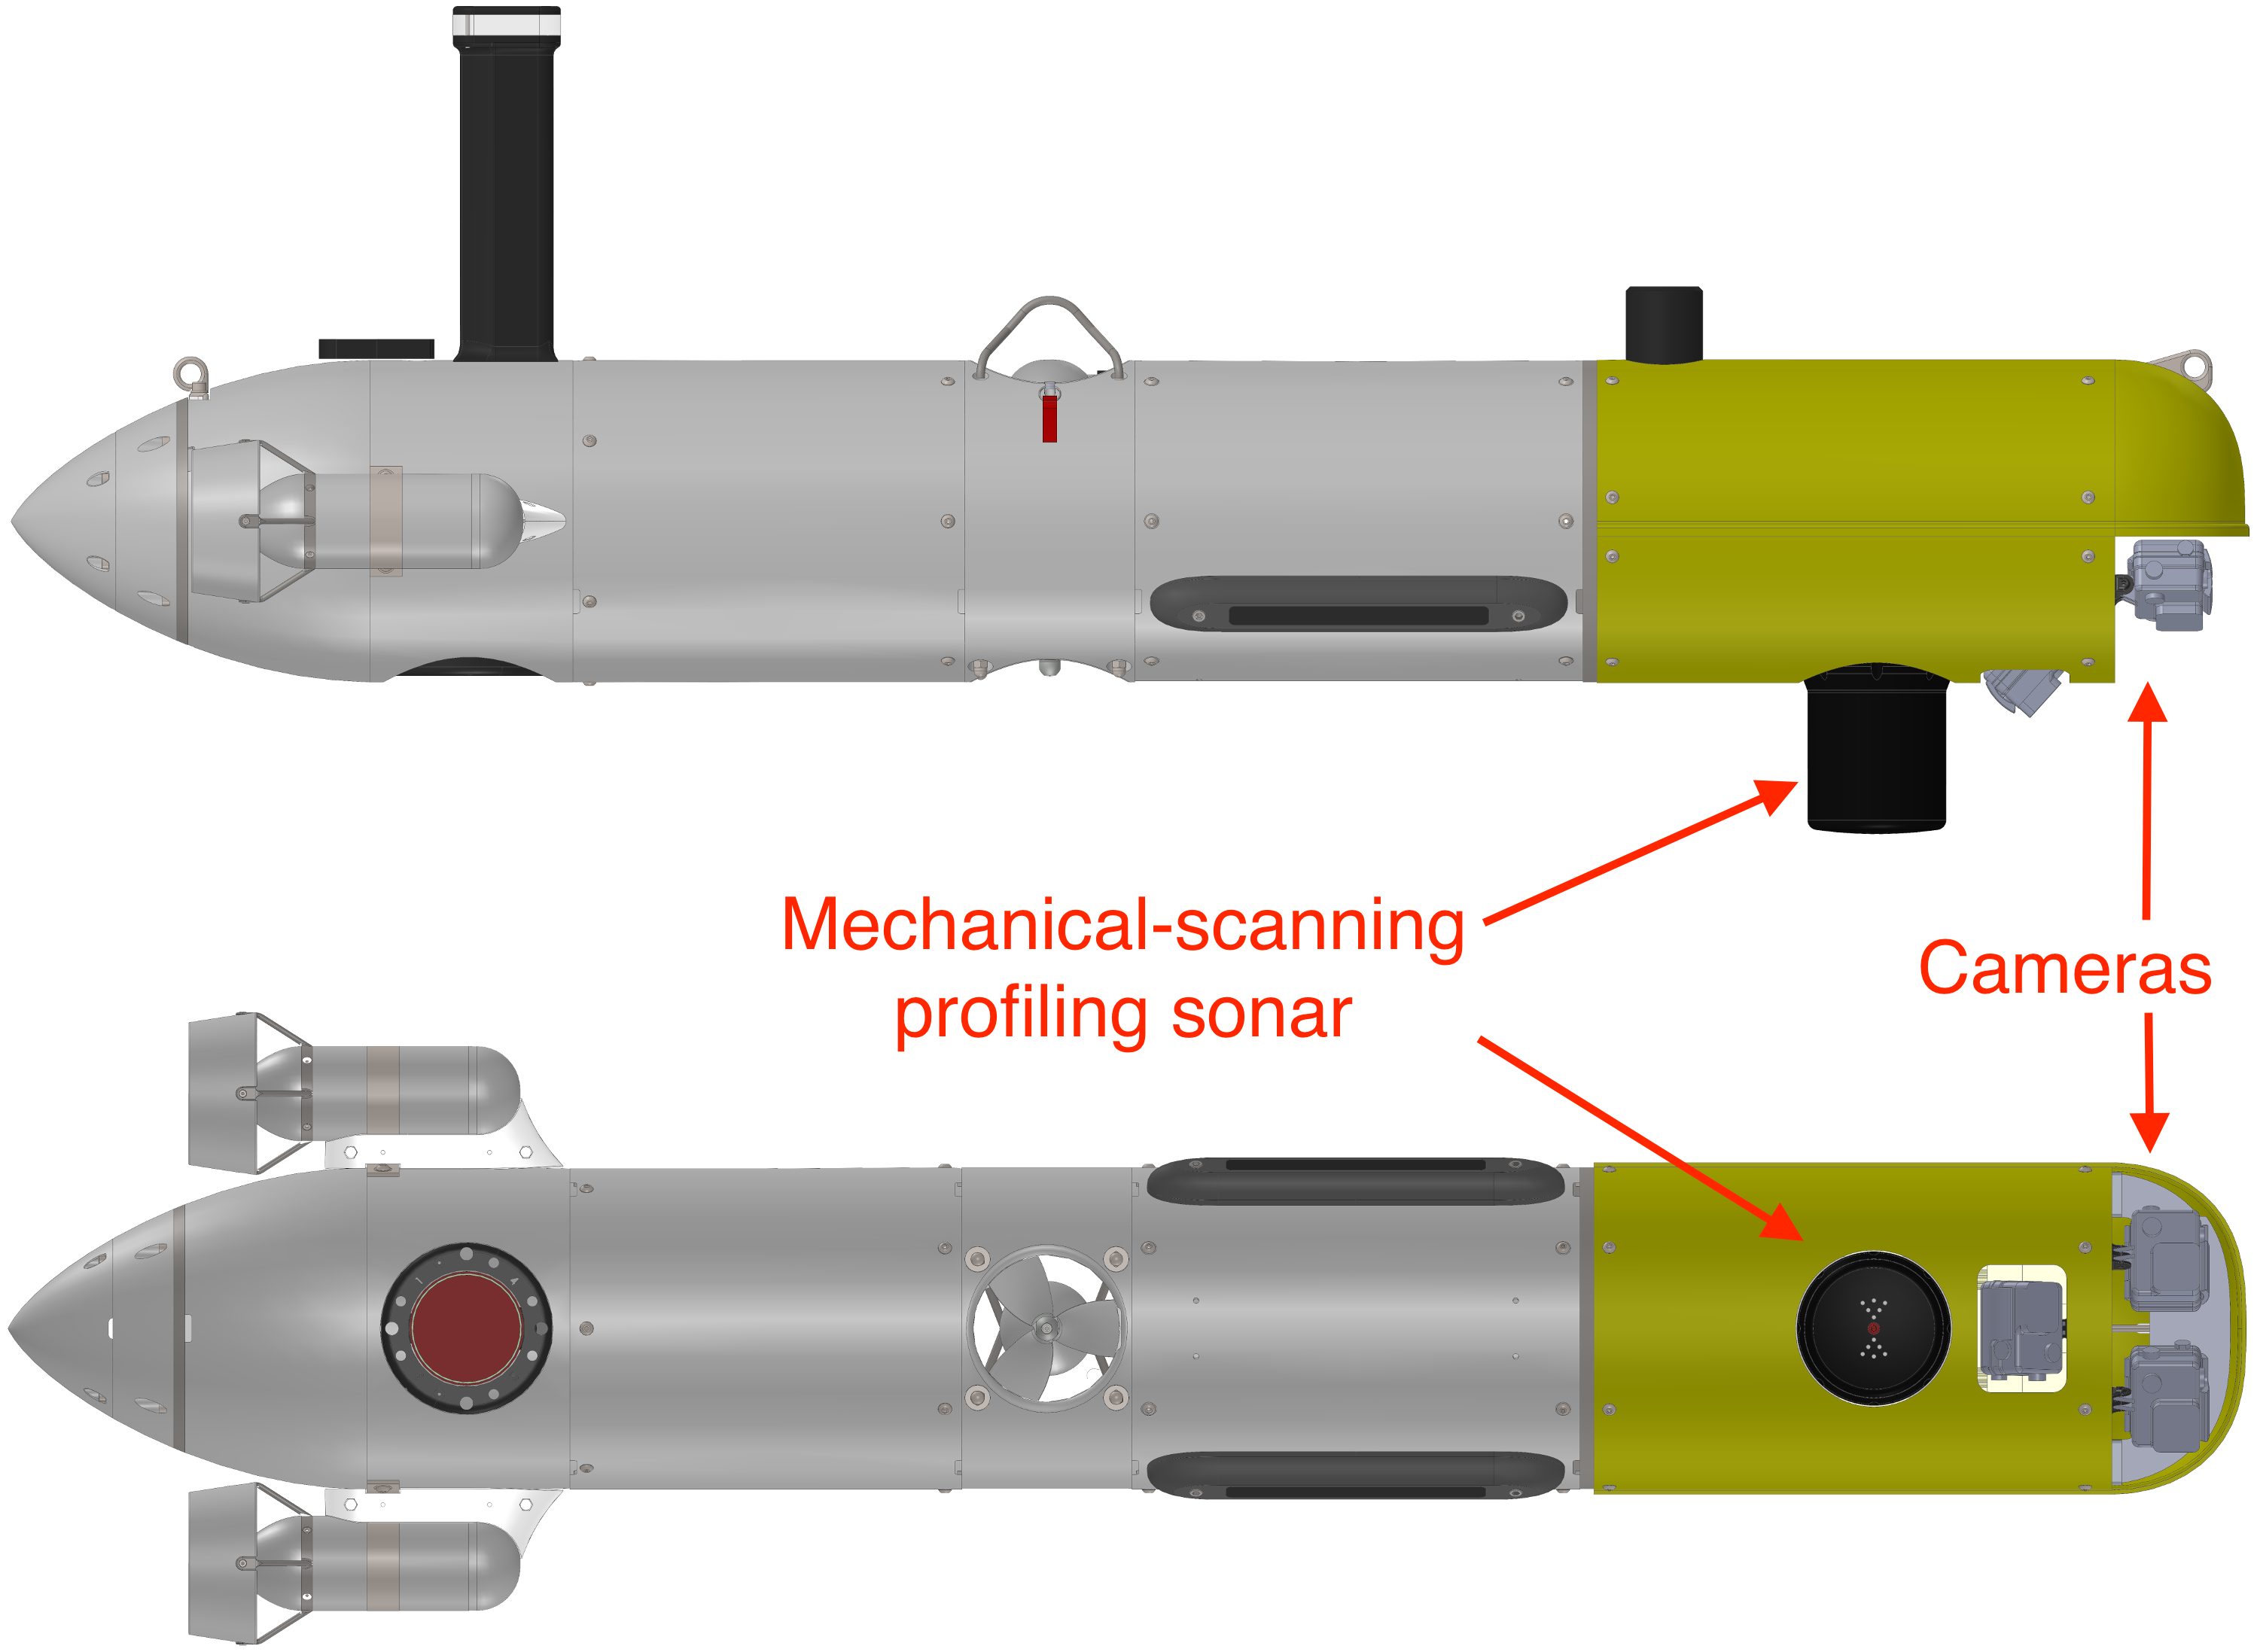
\includegraphics[width=.47\linewidth]{S2PayloadProfilerCameras}}\quad
	\subfloat[]
    {\label{fig:S2PayloadProfCamsReal}
    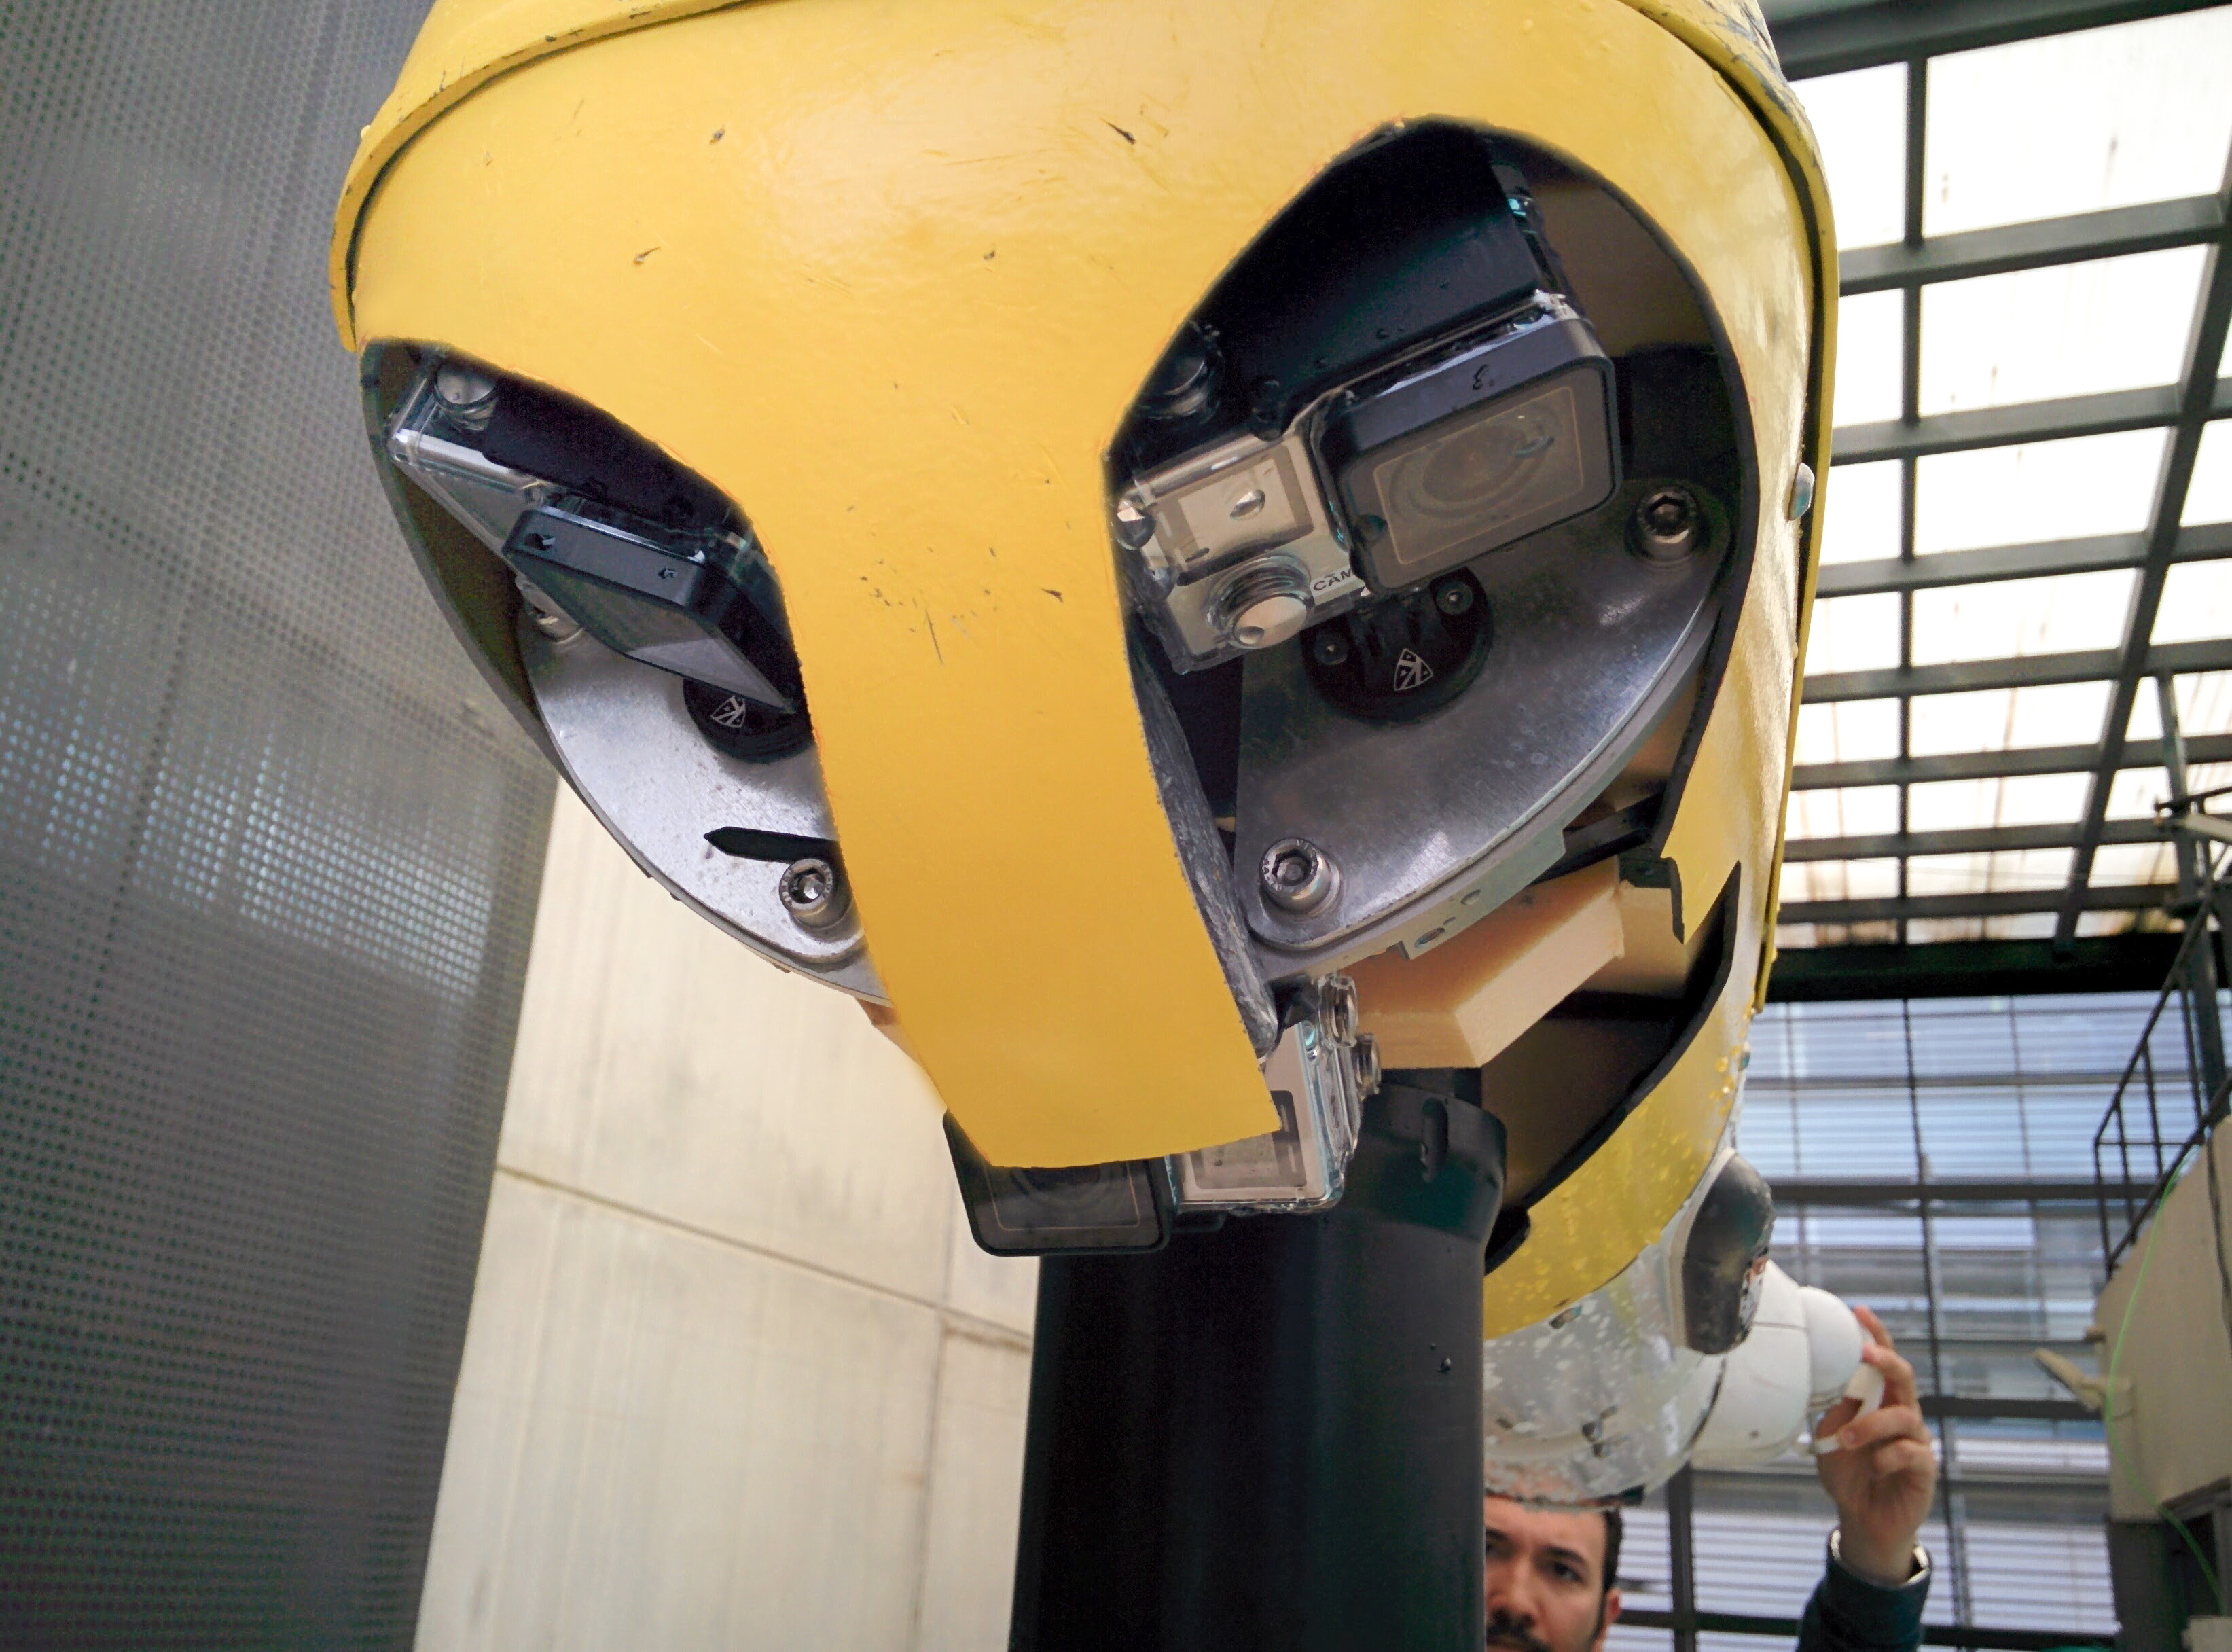
\includegraphics[width=.47\linewidth]{S2PayloadProfCamsReal}}
\caption[Exteroceptive sensors configuration for the Sparus~II AUV to conduct
autonomous missions in the underwater canyon.]
{Exteroceptive sensors configuration for the Sparus~II AUV to conduct autonomous
missions in the underwater canyon.
\protect \subref{fig:S2PayloadProfilerCameras} The vehicle was equipped with
three GoPro\texttrademark{} Hero 4 Black edition cameras and one
mechanical-scanning profiling sonar.
\protect \subref{fig:S2PayloadProfCamsReal} Real-world vehicle's payload.}
\label{fig:S2ProfCamsPayloadConf}
\end{figure}

In order to inspect the underwater canyon and the surroundings, two different
start-to-goal queries were established by extracting GPS coordinates from Google
Maps \copyright. The first query required the Sparus~II \ac{AUV} to traverse the
canyon towards the shore. The second query goal was chosen on the outside of the
rocky formation in such a way that the vehicle had to circumnavigate the outer
rock. Furthermore, after completing the second query, the first query was
executed again until the vehicle overlapped its initial trajectory in the
canyon. This allowed us to verify the navigation consistency and to close the
imaging acquisition loop, thus improving the reconstruction results. As the
profiling sonar covered the horizontal plane, the mission had to be conducted at
a constant depth.

Figure~\ref{fig:SPARUS-Canyon-Scenario} depicts one of the inspection missions
conducted at $3m$ of depth in the underwater canyon. The Sparus~II not only
created a map of a complex and unexplored environment, but also planned a
collision-free path simultaneously and incrementally. The map and the vehicle
trajectory are shown overlapped with a satellite image. In the initial part of the
mission, \ie when the vehicle traverses the canyon for the first time, the map
coincides with the satellite image (see
Fig.~\ref{fig:S2CanyonMultS2GQ1_2}); however, disparities can be
clearly observed after some time (see
Figs.~\ref{fig:S2CanyonMultS2GQ2},~d). Such differences are due to
the accumulation of error in the navigation system that depends on the \ac{DVL},
which may provide incorrect data when navigating over rocks, as occurred in this
test scenario. Despite this situation, the vehicle succeeded in conducting the
mission because both the map and the path are created online, which permits
correcting or adjusting them even when moving in previously visited areas (see
Fig.~\ref{fig:S2CanyonMultS2GQ3} when accessing the canyon for a
second time).

\begin{figure}[htbp]
\myfloatalign
   	\subfloat[]{
		\label{fig:S2CanyonMultS2GQ1_1}
   		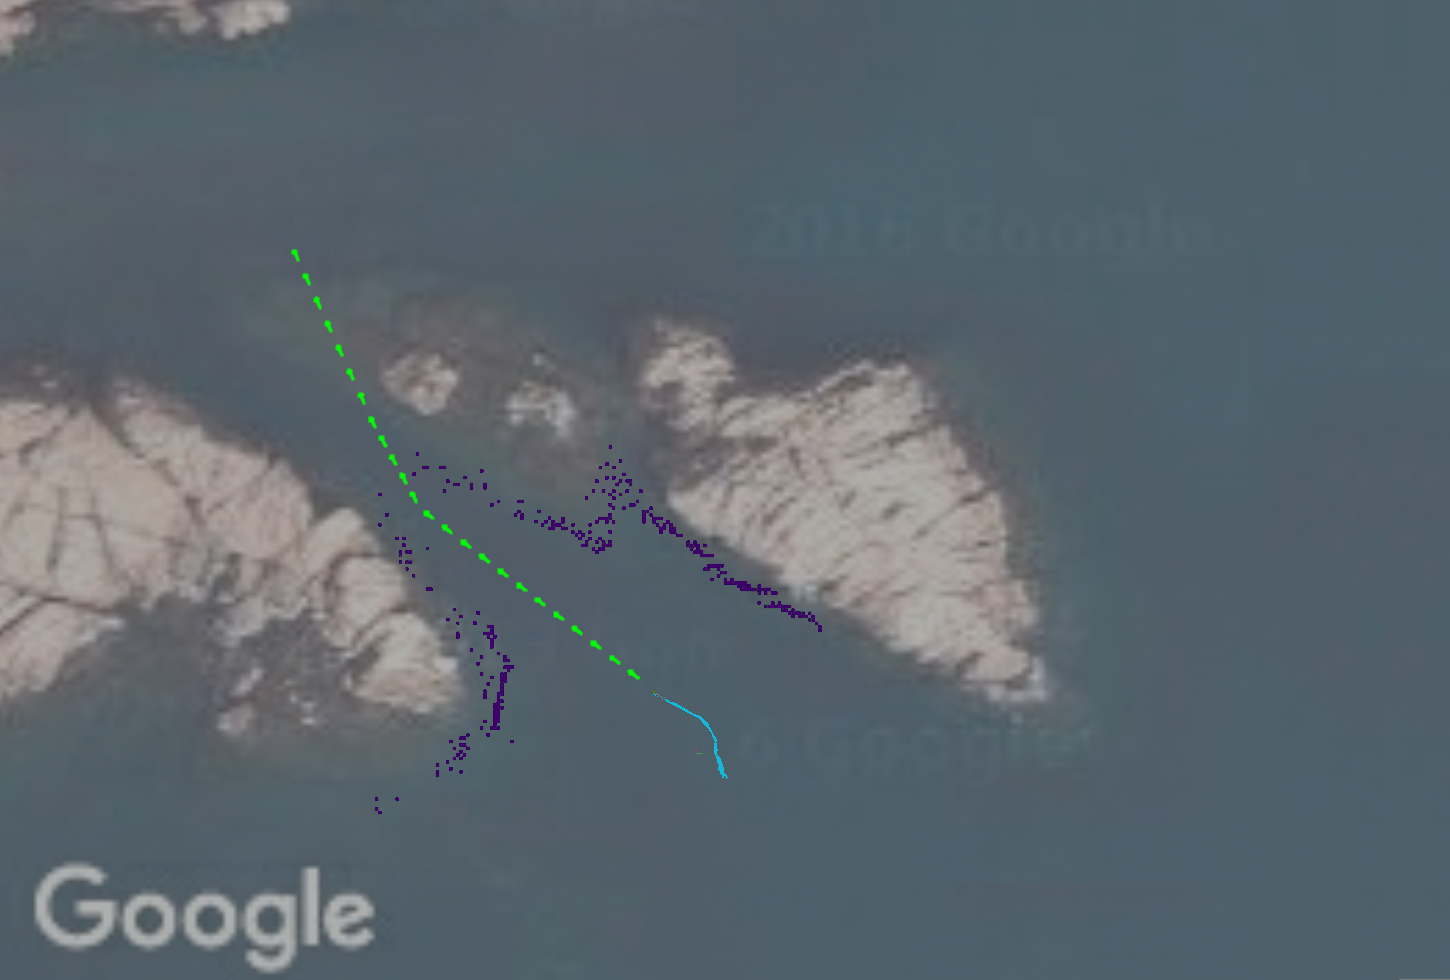
\includegraphics[width=.45\linewidth]{S2CanyonMultS2GQ1_1}}\quad
   	\subfloat[]{
		\label{fig:S2CanyonMultS2GQ1_2}
   		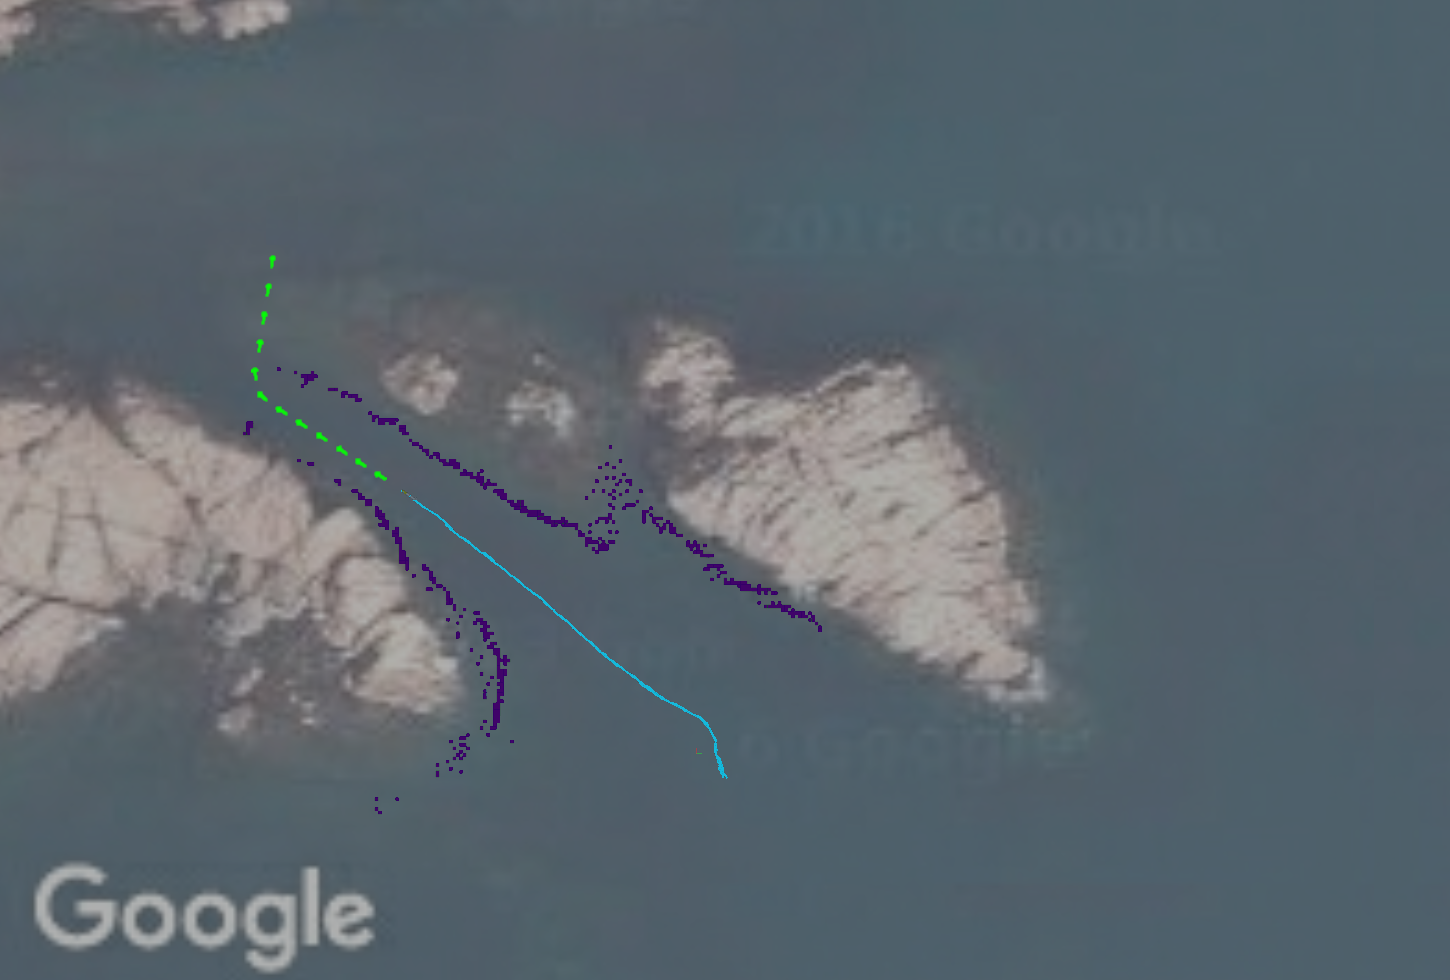
\includegraphics[width=.45\linewidth]{S2CanyonMultS2GQ1_2}}\\
   	\subfloat[]{
		\label{fig:S2CanyonMultS2GQ2}
   		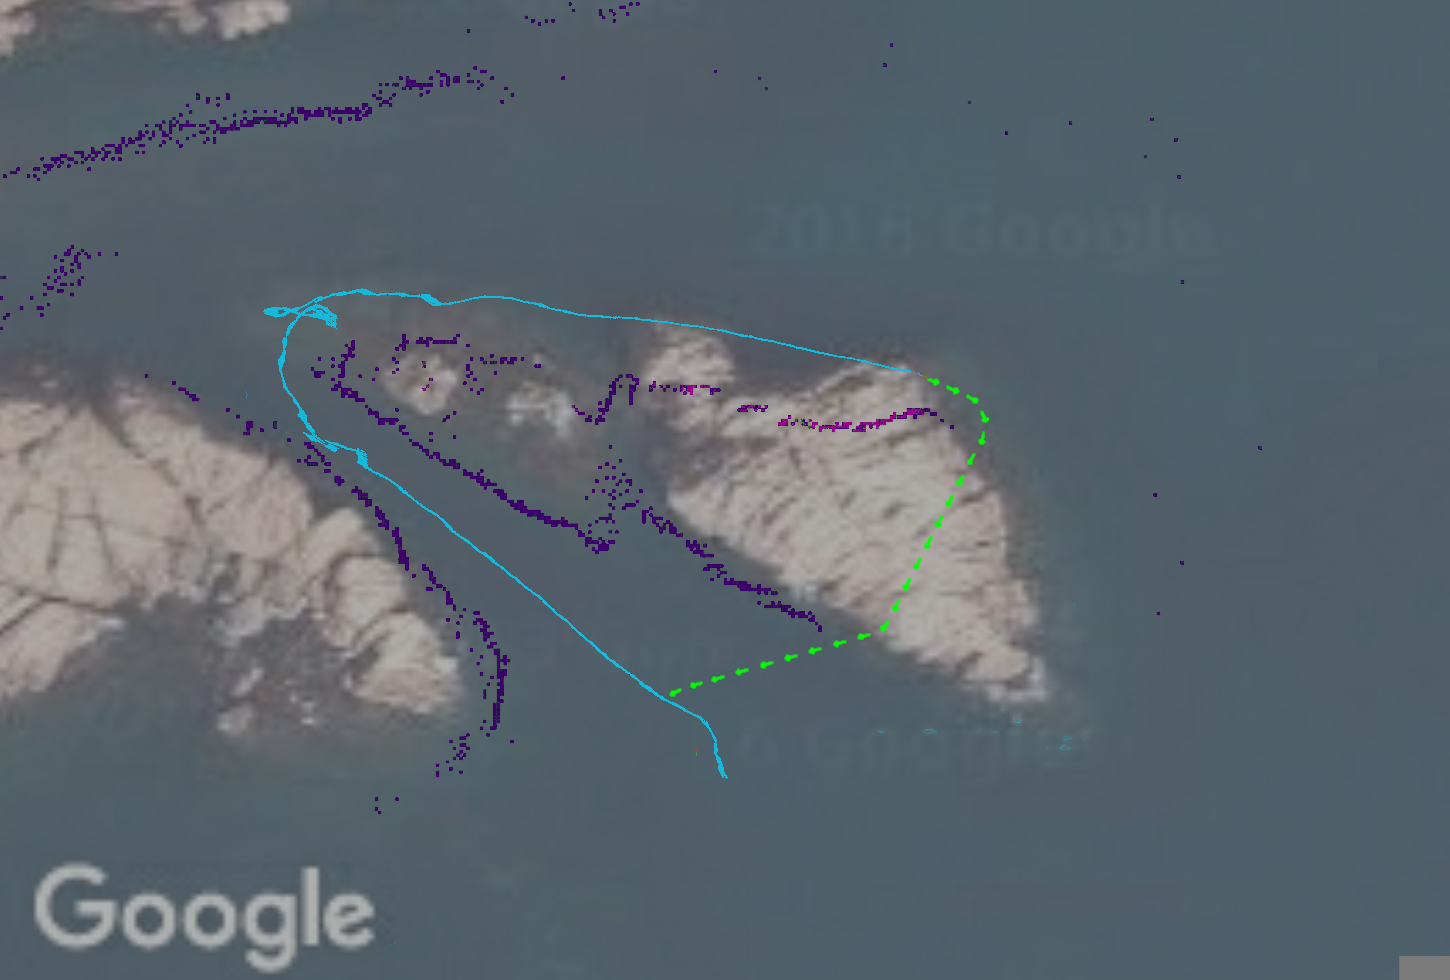
\includegraphics[width=.45\linewidth]{S2CanyonMultS2GQ2}}\quad
   	\subfloat[]{
		\label{fig:S2CanyonMultS2GQ3}
   		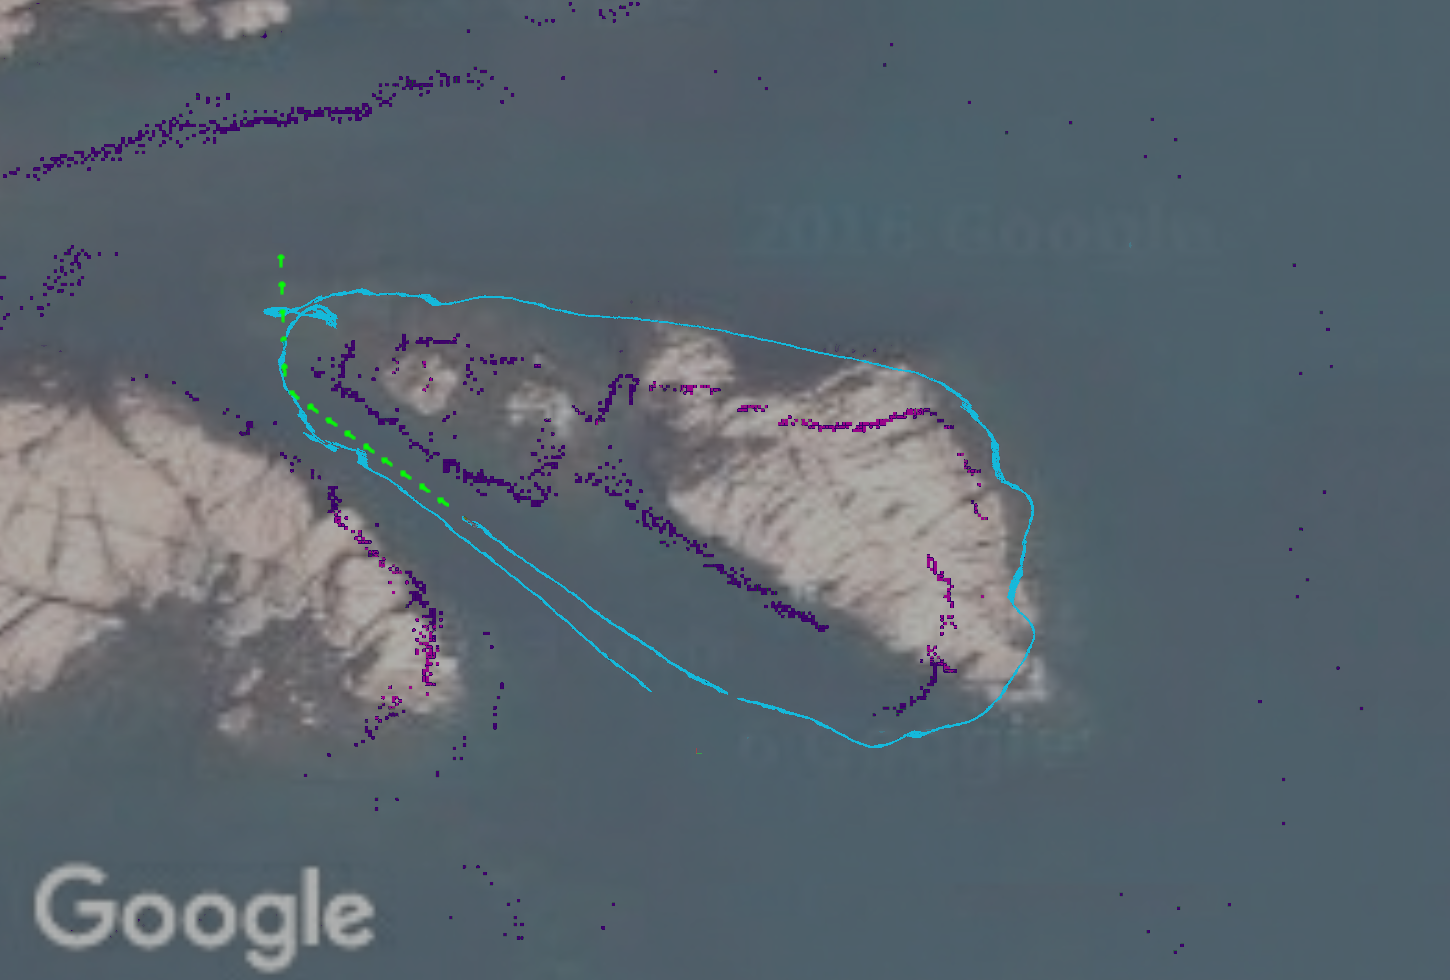
\includegraphics[width=.45\linewidth]{S2CanyonMultS2GQ3}}
\caption[The Sparus II AUV using the path/motion planning framework to navigate
through an underwater canyon without a preliminary map of the surroundings.]
{The Sparus II \ac{AUV} used the path/motion planning framework to navigate
through an underwater canyon without a preliminary map of the surroundings.
\protect \subref{fig:S2CanyonMultS2GQ1_1}, \protect
\subref{fig:S2CanyonMultS2GQ1_2} The first start-to-goal query required
the Sparus~II traversing an underwater canyon.
\protect \subref{fig:S2CanyonMultS2GQ2} For the second query, the vehicle
circumnavigated the outer rock. 
\protect \subref{fig:S2CanyonMultS2GQ3} The AUV partially repeated the
first start-to-goal query in order to close the loop and to obtain overlapped
images. Vehicle trajectory and Octomap overlap a satellite image (Map
data \copyright 2017 Google).}
\label{fig:SPARUS-Canyon-Scenario}
\end{figure}

In this kind of explorations, the data that is gathered along the mission can be
used to create a more detailed survey of the area. In this particular
mission, for instance, the images were extracted and were used to build a
photo-realistic \ac{3D} model, which is depicted in
Figure~\ref{fig:3Drecon_top}. This \ac{3D} reconstruction allows us to better
understand complex environments by generating arbitrary user-defined views (see
Figs~\ref{fig:3D_reconstruction_texture}b--d). For more details about these
\ac{3D} reconstructions, the interested reader is referred
to~\cite{Hernandez2016,Hernandez2016a}.

\begin{figure}[htbp]
\myfloatalign
	\subfloat[]{
		\label{fig:3Drecon_top}
   		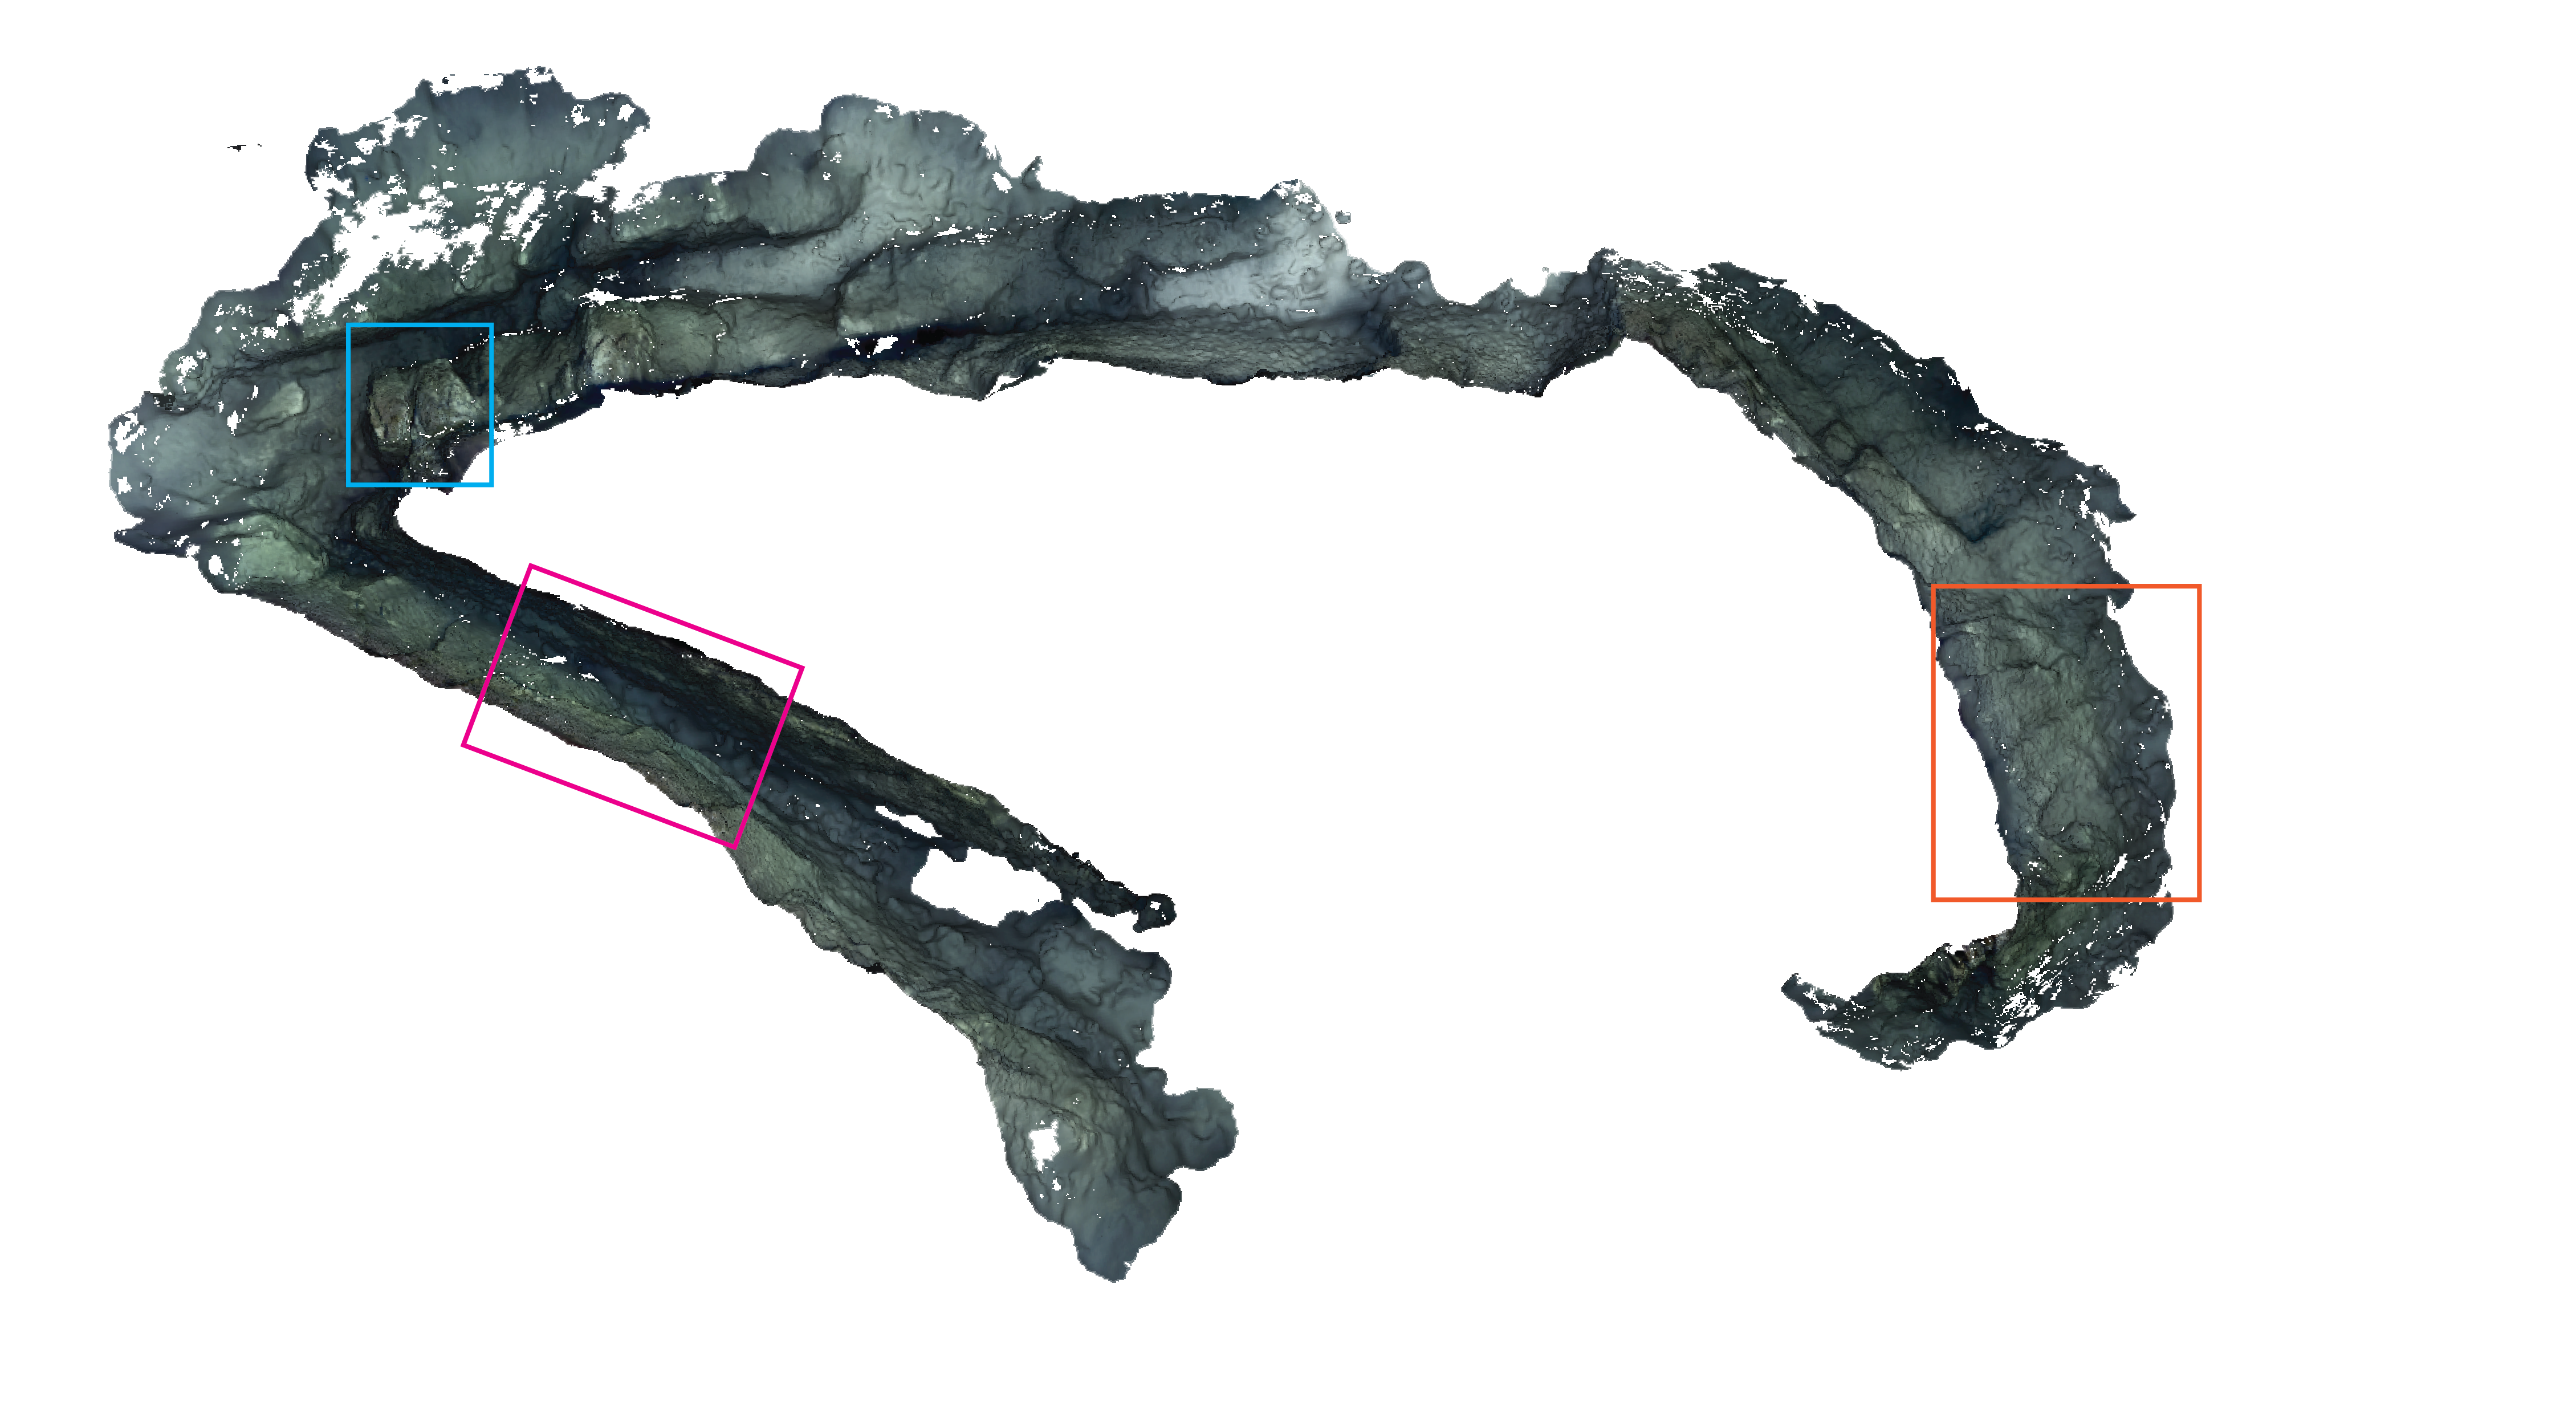
\includegraphics[width=.9\linewidth]{3D_topdown_marked.png}}\\
   	\subfloat[]{
		\label{fig:3Drecon_arb_A}
   		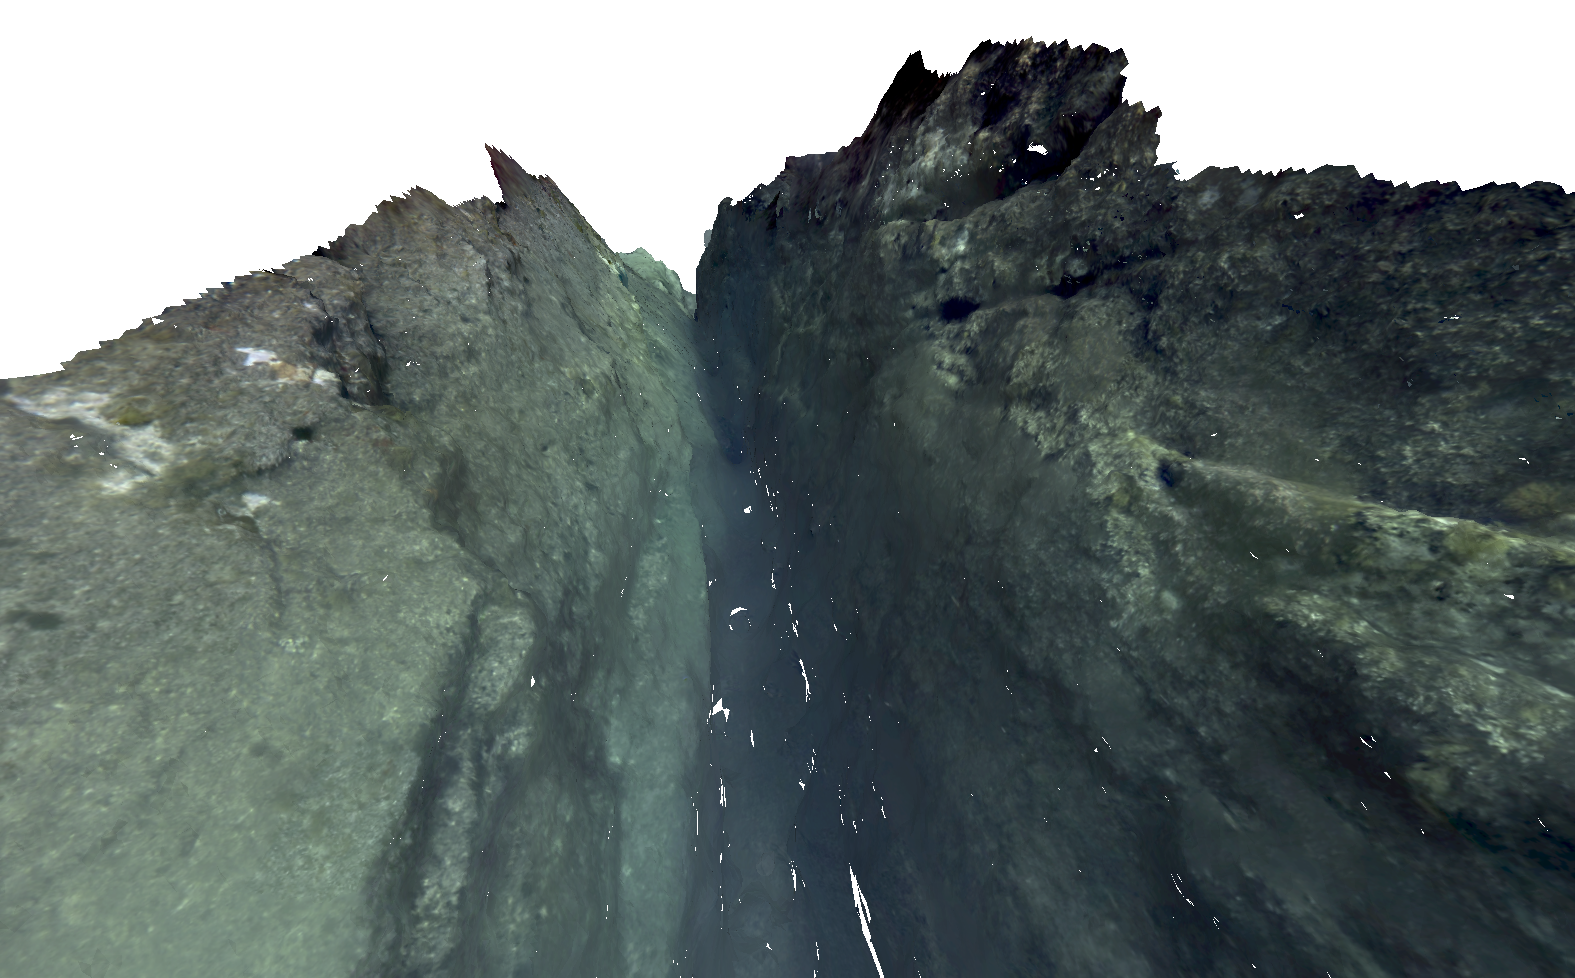
\includegraphics[width=.43\linewidth]{3D_canyon.png}}\quad
   	\subfloat[]{
		\label{fig:3Drecon_arb_B}
   		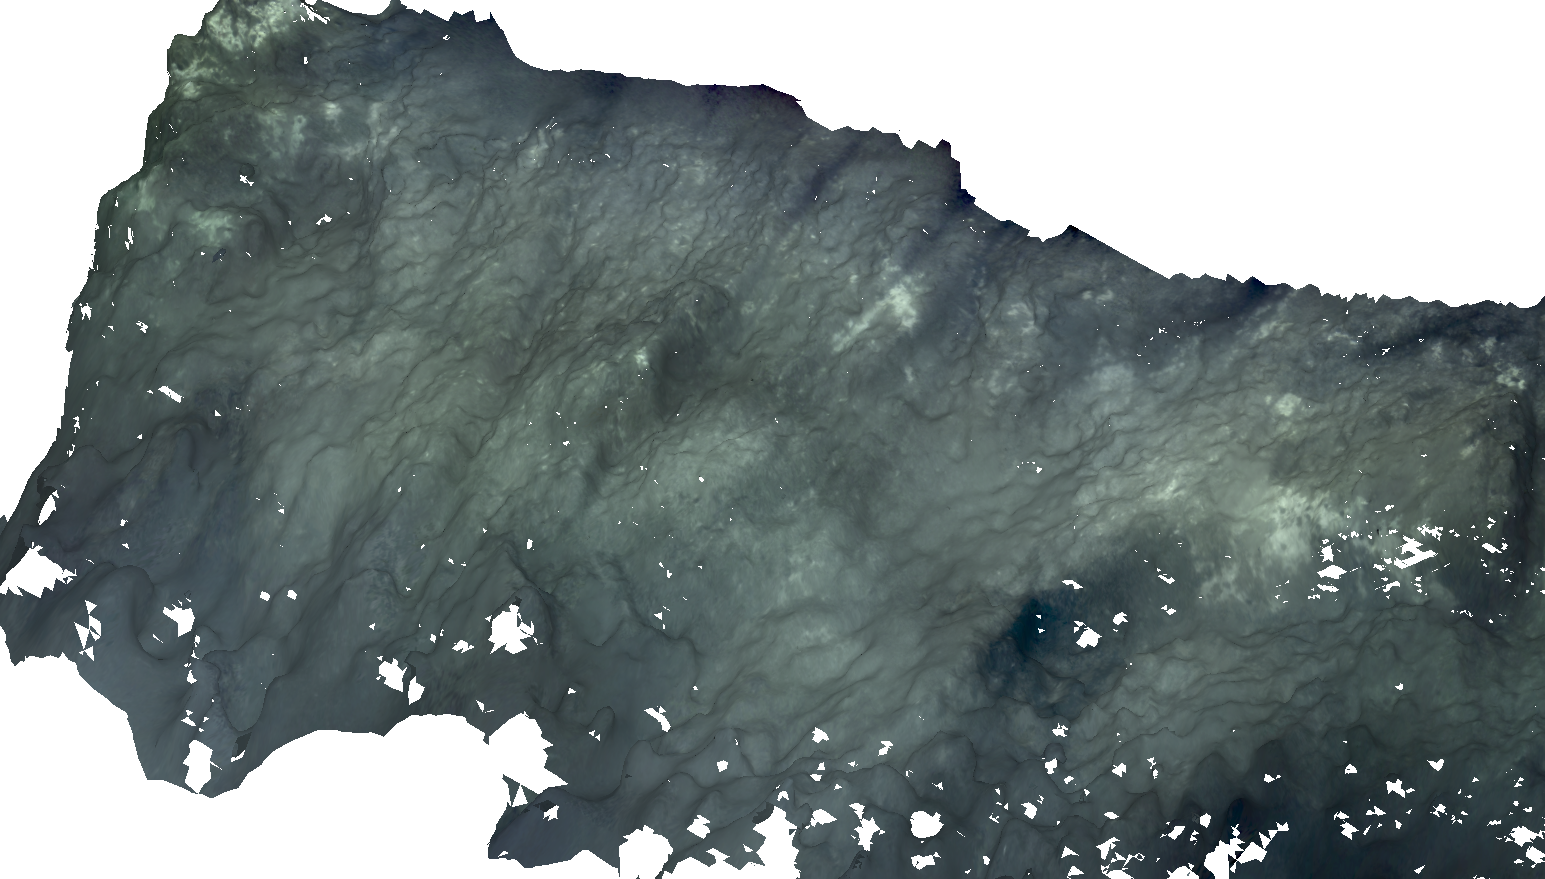
\includegraphics[width=.43\linewidth]{3D_outside.png}}\\
   	\subfloat[]{
		\label{fig:ReconCamType_tex_zoom}
   		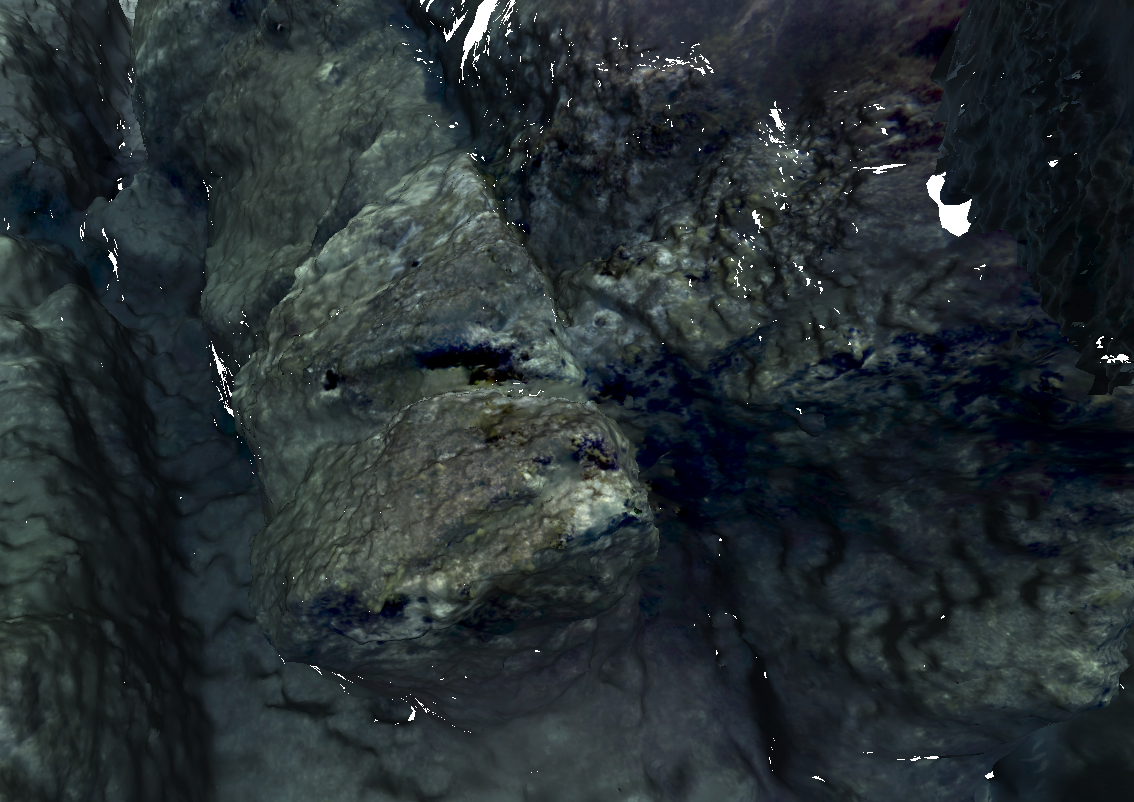
\includegraphics[width=.5\linewidth]{camType_tex_zoom.png}}
\caption[3D reconstruction built from images gathered along the autonomous
mission presented in Fig.~\ref{fig:SPARUS-Canyon-Scenario}.]
{\protect \subref{fig:3Drecon_top} Top-down view of the textured 3D model with
marked areas additionally depicted in magenta, orange and blue, which
correspond to generated views of:
\protect \subref{fig:3Drecon_arb_A} the underwater canyon; 
\protect \subref{fig:3Drecon_arb_B} the external side of the underwater rocky
formation; \protect \subref{fig:ReconCamType_tex_zoom} underwater rocks.}
\label{fig:3D_reconstruction_texture}
\end{figure}

Finally, in order to understand the complexity associated with this mission,
Figure~\ref{fig:SPARUS-Overlapped-Trajectories} presents a visual comparison
between the vehicle's trajectory, estimated by its \ac{DR} system, and the
cameras' trajectory, estimated during the reconstruction (green and red,
respectively). While both trajectories have a similar shape, it can be clearly
observed how the one derived from the cameras is more realistic according to the
rock observed in the surface (the rocky formation does not create a vertical
wall, which means that the vehicle may have moved further from the visible part
of the rock when navigating at $3m$ deep), while the one estimated by the
\ac{AUV}'s dead-reckoning system seems to be colliding with the rock. This
latter situation is mainly due to the accumulation of errors in the navigation
system, as it was already mentioned before.

\begin{figure}[htbp]
\myfloatalign
	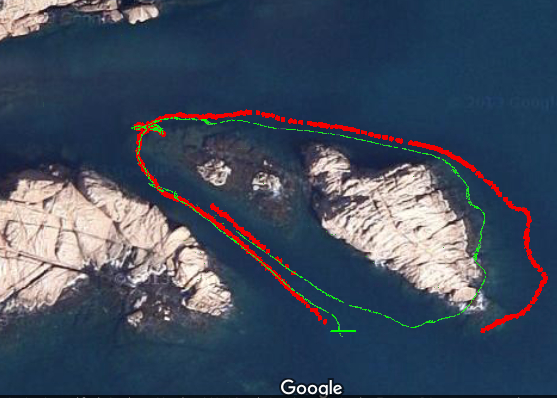
\includegraphics[width=.6\linewidth]{SPARUS-Real-Canyon-Scenario5}
\caption[Comparison between the vehicle trajectory estimated by the DR system
and the one estimated with the cameras' images.]
{Vehicle trajectory (green) calculated by its dead-reckoning system and the
cameras trajectory (red) estimated by the image-based reconstruction. Both
trajectories are shown overlapped with a satellite image of the test scenario (Map
data \copyright 2017 Google).}
\label{fig:SPARUS-Overlapped-Trajectories}
\end{figure}

\section{Planning AUV Paths in Confined Natural Environments}
\label{sec:caves_experiments}

The experiments that have been presented until now involved the Sparus~II
navigating at a constant depth. However, there are other scenarios in which the
\ac{AUV} must modify its vertical position in order to complete the intended
mission. In such cases, one of the main limitations from the mapping and
path-planning perspective is the capability to build online a \ac{3D} map of the
surroundings. As explained in Sec.~\ref{sec:MappingModule}, Octomaps offer an
efficient alternative to represent volumetric environment information. Such data
can be gathered from a wide range of sensors such as echosounders,
profiling/imaging sonars, and multibeam sonars.

One example of a mission that require a \ac{3D} path/motion planner is to move
through confined natural environments (\eg underwater caves and tunnels). This
kind of scenarios present all sort of limitations, including the impossibility
of having either a support surface ship to correct the \ac{AUV} navigation
through an \ac{USBL} system, or even a wireless access point buoy for monitoring
the correct mission execution. Other technical aspects that make more difficult
to conduct autonomous missions in these environments, include the navigation
error associated with incorrect data provided by the \ac{DVL} when traveling
over rocky surfaces.

In dealing with this latter aspect, Mallios \etal presented the exploration of
an underwater caves complex (see Fig.~\ref{fig:CavesSatellite}), in which a
diver guided the Sparus \ac{AUV} to gather environment acoustic
information~\cite{Mallios2015}. To do so, the vehicle was equipped with two
mechanically scanning imaging sonars to cover the horizontal and vertical
planes. Such data was used to prove a scan-matching algorithm over a \acf{SLAM}
framework, which allows reducing and bounding the \ac{AUV} navigation error.
This survey provides an extensive dataset that includes not only the sonars' raw
data, but also a detailed meshed map (see
Fig.~\ref{fig:Caves3DMesh})~\cite{Mallios2015,Mallios2017}. This latter one was
obtained by using the \ac{SDNC} algorithm~\cite{Campos2013}. For more details
about this survey, the interested reader is referred to the cited references.

\begin{figure}[htbp] %  figure placement: here, top, bottom, or page
\centering
	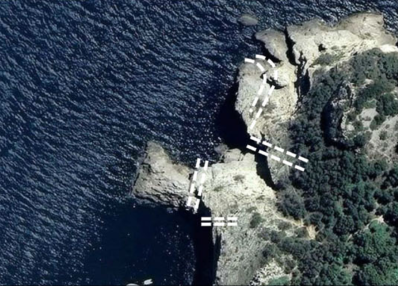
\includegraphics[width=.7\linewidth]{CavesSatellite}
\caption[Satellite image of the underwater caves complex ``Coves de Cala
Viuda''.]
{Satellite image of the dataset area. The underwater caves complex ``Coves de
Cala Viuda'' is located in the L'Escala, Spain (Lat: 42.10388, Lon: 3.18255). It
consists of three single-branch caves and several tunnels. Their approximate
positions are marked with dotted white lines.
Image credit: Mallios \etal 2015~\cite{Mallios2015, Mallios2017}}
\label{fig:CavesSatellite}
\end{figure}

All this together is nowadays considered a significant step towards the
exploration of these kinds of environments. Nonetheless, there are still other
aspects that must be tackled in order to conduct this kind of missions fully
autonomous. This thesis contributes to coping with some of those aspects. The
proposed framework, for instance, seeks to endow \acp{AUV} with additional
capabilities that will allow to replace the diver's guidance in a near future.
To prove these capabilities, this section presents a simulated mission over the
meshed map of the cave complex. The mission consisted in solving six consecutive
start-to-goal queries, where the Sparus~II was not provided with any preliminary
environment information, thus requiring to incrementally map and (re)plan the
path to the goals. Figure~\ref{fig:Caves3DMesh} depicts the meshed map and the
approximate locations of six different query goals.

\begin{figure}[htbp] %  figure placement: here, top, bottom, or page
\centering
	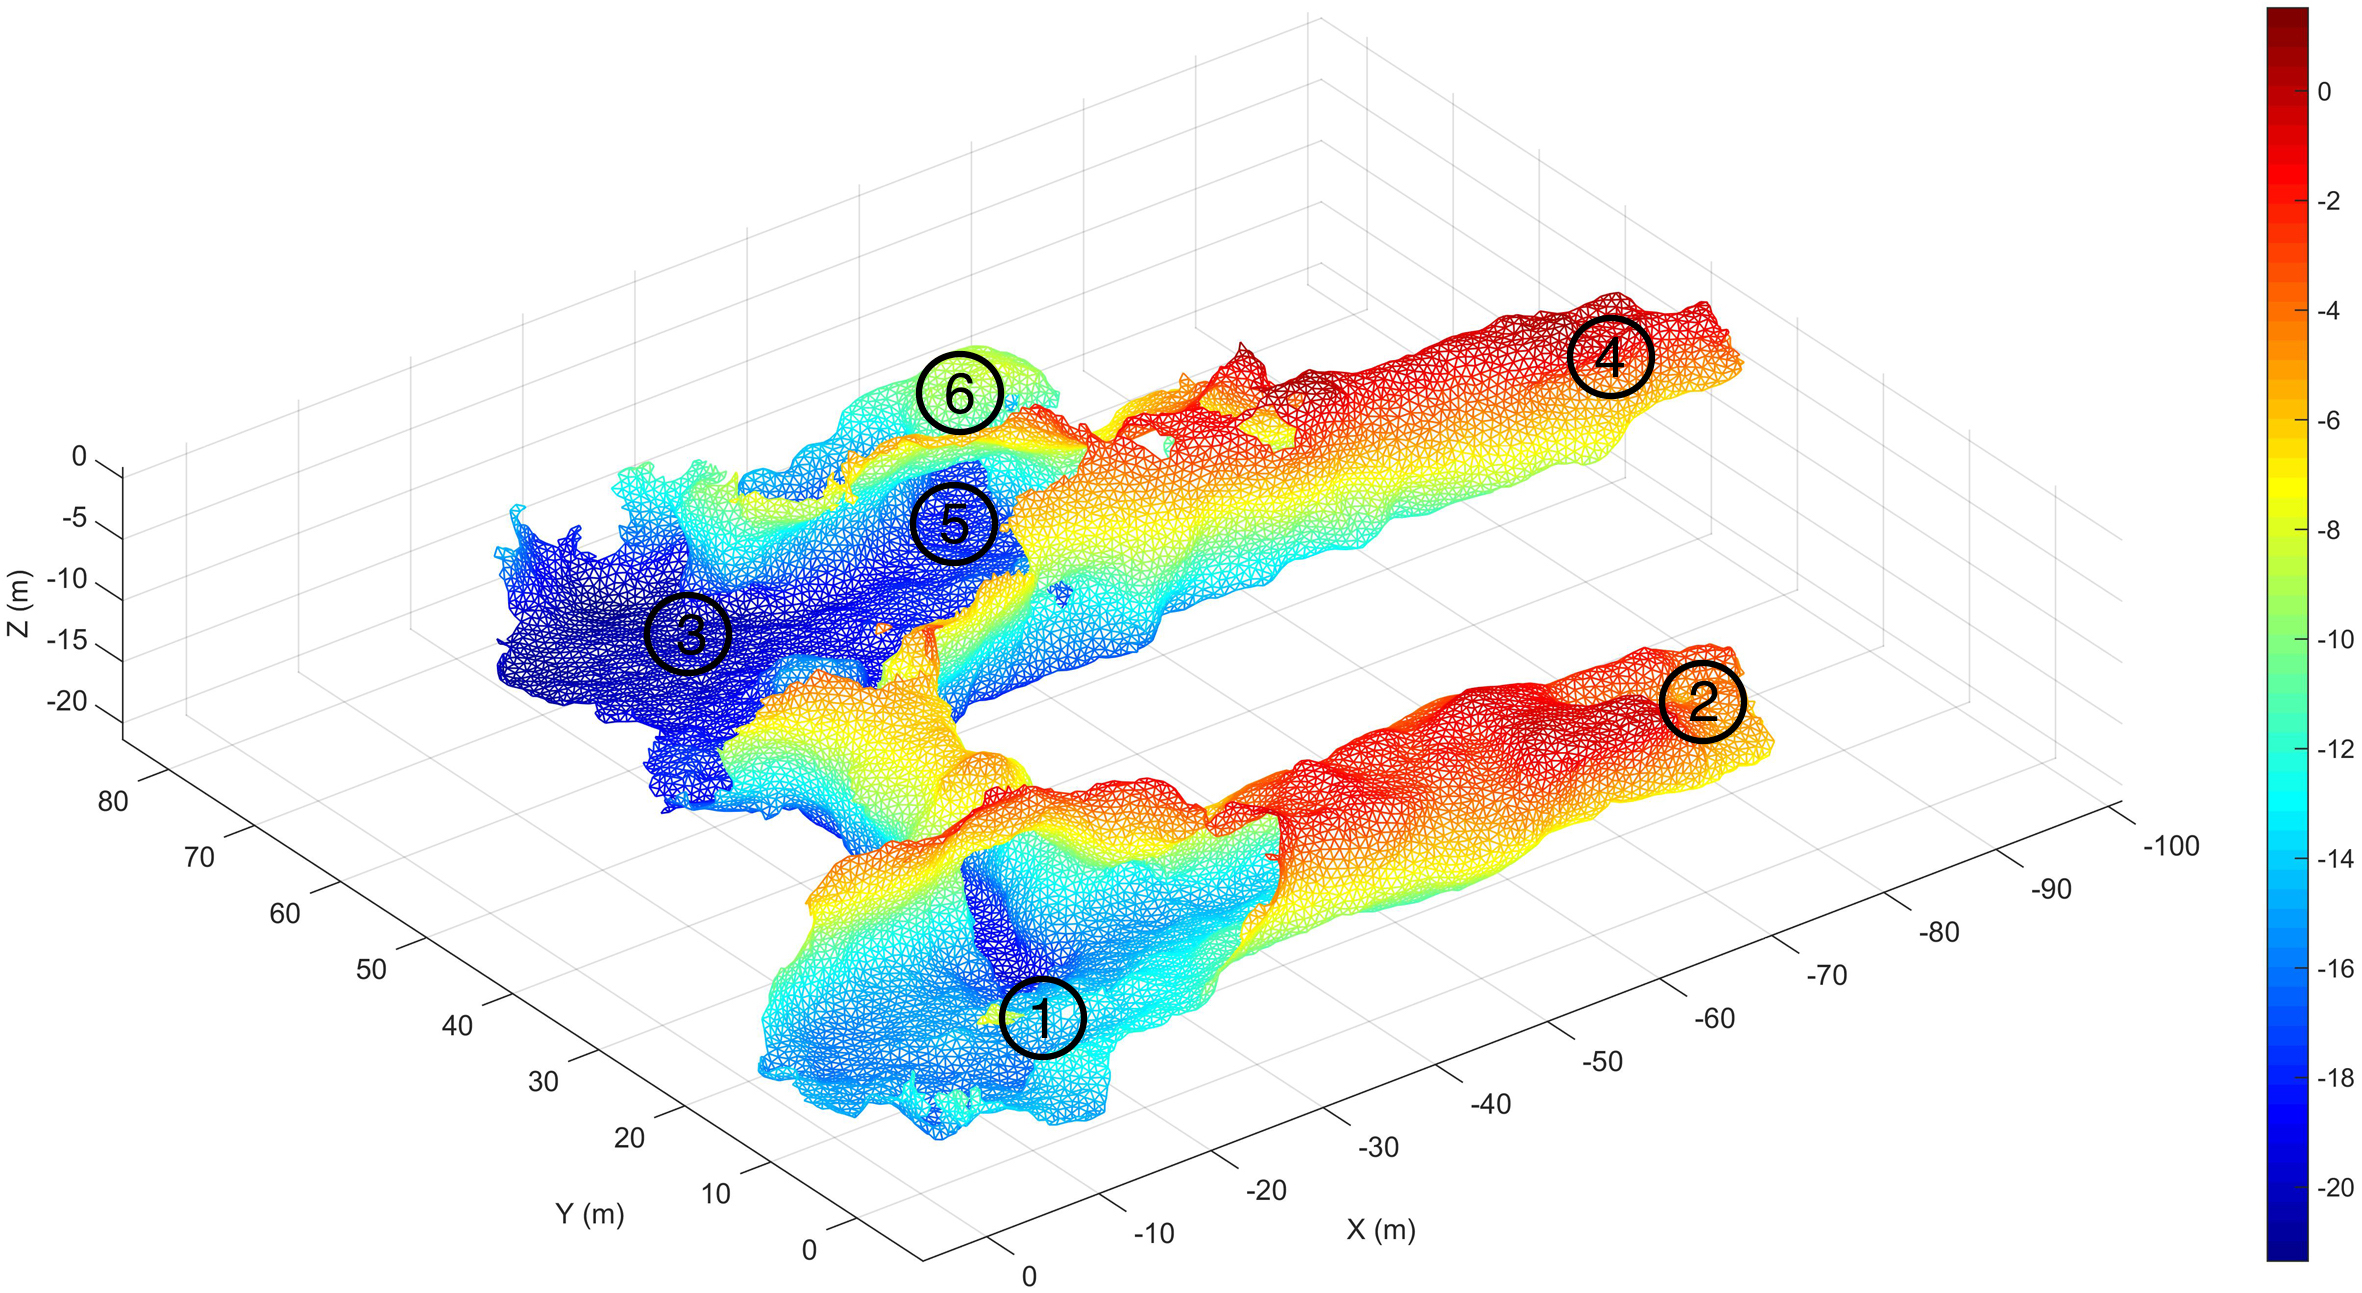
\includegraphics[width=.95\linewidth]{Caves3DMesh}
\caption[The underwater caves complex ``Coves de Cala Viuda''. Meshed map
constructed using the SNDC algorithm.]
{The underwater caves complex ``Coves de Cala Viuda''. Meshed map using the SNDC
algorithm~\cite{Campos2013}. Image credit: Mallios \etal
2015~\cite{Mallios2015}. Over the map, the approximate locations of six
different goals have been marked in black.}
\label{fig:Caves3DMesh}
\end{figure}

In order to conduct this test mission, the meshed map was added into \ac{UWSim}
as a \ac{3D} simulation environment (see Fig.~\ref{fig:CavesUWSim}). To perceive
the surroundings, the \ac{AUV}'s payload was assumed to be equipped with an
additional link capable of rotating $120^o$ around the vehicle's $z$ axis.
Over this link, a forward-looking multibeam sonar was mounted. The sonar had
$240$ beams distributed over a total aperture of $120^o$ around the vehicle's
$x$ axis. With this payload configuration, the simulated Sparus~II was capable
of gathering \ac{3D} range data of the environment along its direction of
motion.

\begin{figure}[htbp] %  figure placement: here, top, bottom, or page
\centering
	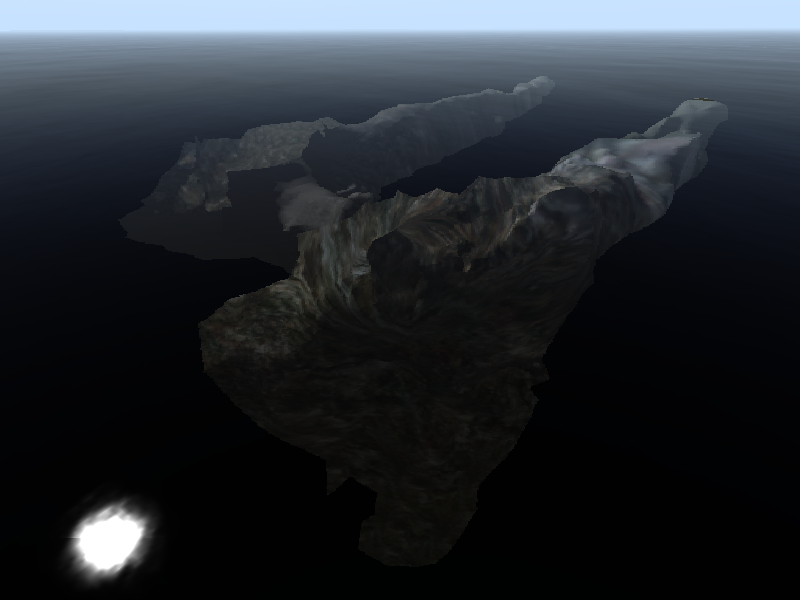
\includegraphics[width=.8\linewidth]{CavesUWSim}
\caption[The underwater caves complex ``Coves de Cala Viuda'' added into UWSim
as a 3D simulation environment.]
{The underwater caves complex ``Coves de Cala Viuda'' added into \ac{UWSim} as a
\ac{3D} simulation environment.}
\label{fig:CavesUWSim}
\end{figure}

At the beginning of the mission, the simulated Sparus~II was located at the
origin of the \ac{NED} reference system and oriented towards the north, \ie
$q_{start} = [0.0, 0.0, 0.0, 0.0]$. The first start-to-goal query was defined to
guide the \ac{AUV} closer to the caves complex location. This required setting
$q_{goal_1} = [20.0, 0.0, 12.0, 0.0]$. From this latter position, the second
query sought to explore the first and biggest single-branch cave. This meant
navigating through and until the end of the cave, which required setting
$q_{goal_2} = [18.0, 55.0, 8.0, 1.57]$. For these queries, the planner limited
the vehicle to navigate at a constant surge speed $v=0.5m/s$, a maximum
ascending speed $d_{ascend}=0.2m/s$, and a maximum descending speed
$d_{descend}=0.18m/s$. Figure~\ref{fig:CavesMultS2G_Q2} depicts part of the
execution of these two queries, including the \ac{AUV} trajectory, the
calculated path, and the goals.

\begin{figure}[htbp]
\myfloatalign
	\subfloat[Vehicle trajectory, calculated path, goals, and Octomap]{
		\label{fig:CavesMultS2G_Q2_RViz}
   		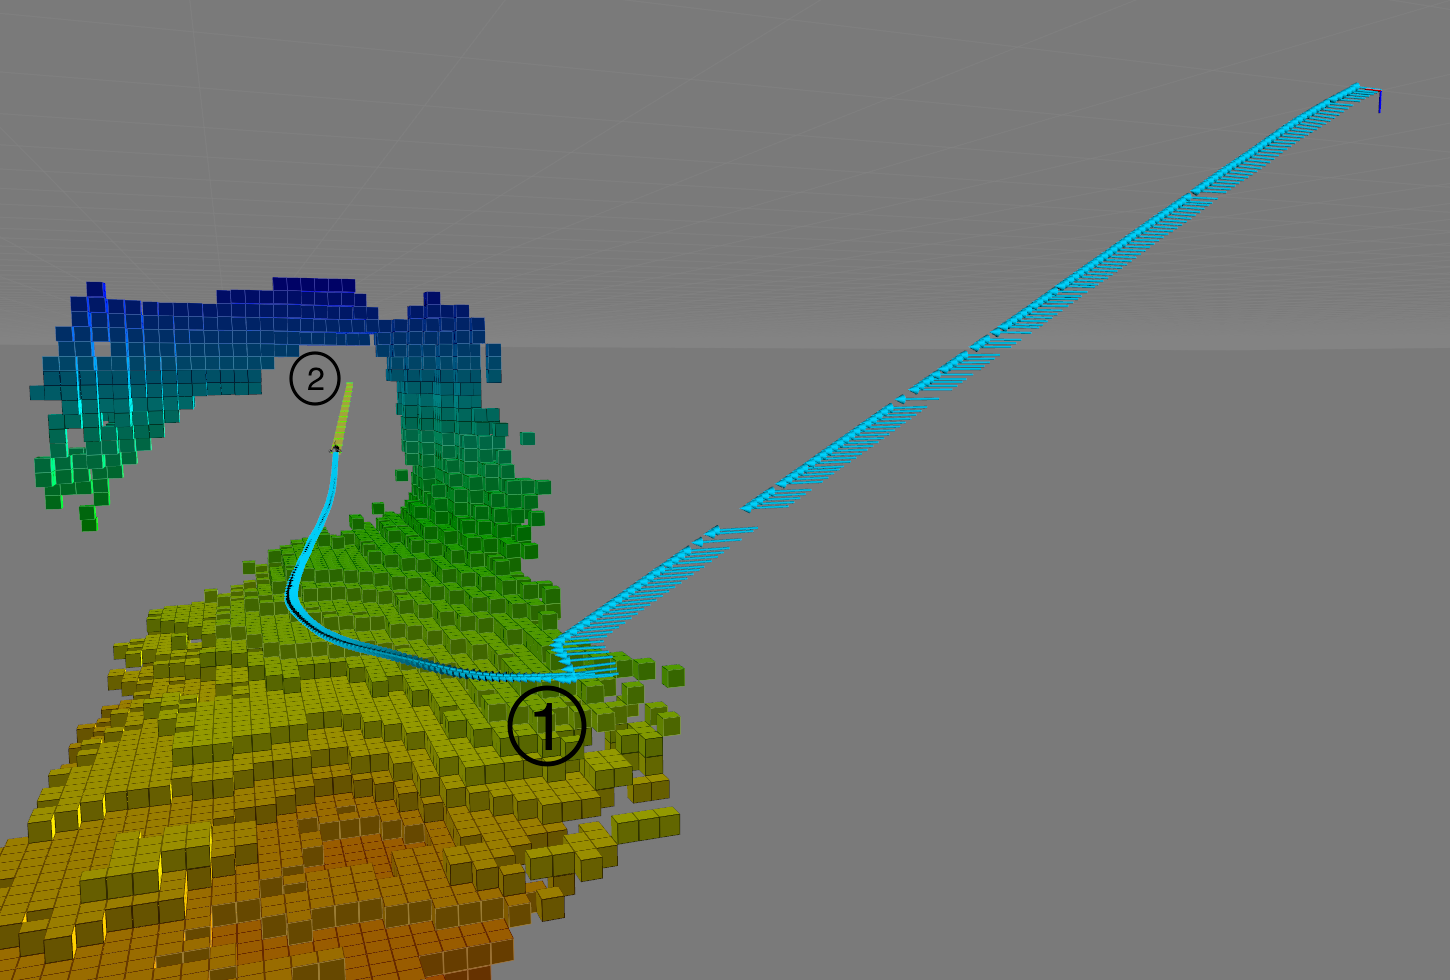
\includegraphics[width=.70\linewidth]{CavesMultS2G_Q2_RViz}}\\
   	\subfloat[Sparus~II approaching the entrance of the first cave]{
		\label{fig:CavesMultS2G_Q2_UWSim}
   		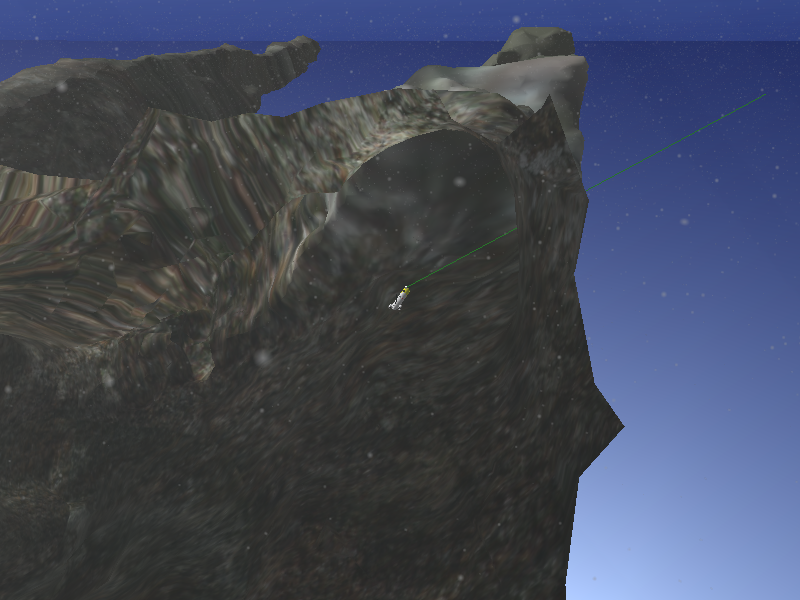
\includegraphics[width=.70\linewidth]{CavesMultS2G_Q2_UWSim}}
\caption[Simulated mission in the caves complex. First and second start-to-goal
queries.] 
{Simulated mission in the caves complex. The first start-to-goal query guided
the \ac{AUV} closer to the complex location. The second query required the
vehicle to navigate through the first single-branch cave. In \protect
\subref{fig:CavesMultS2G_Q2_RViz} The vehicle trajectory appears in light blue,
and the remaining of the calculated path in yellow.}
\label{fig:CavesMultS2G_Q2}
\end{figure}

From the second query's goal configuration, a third query was defined to take
the Sparus~II closer to the second single-branch cave's entrance, \ie
$q_{goal_3} = [80.0, 25.0, 16.0, 0.23]$. To accomplish this part of the mission,
the \ac{AUV} not only had to find a way out of the first cave, but also had to
traverse a tunnel that connects the entrances of both single-branch caves.
For this query, the planner limited the vehicle to navigate at a constant surge
speed $v=0.3m/s$, while keeping the previous maximum ascending/descending speeds
($d_{ascend}=0.2m/s$ and $d_{descend}=0.18m/s$). This decrease of $v$ permitted
the vehicle to conduct maneuvers with a smaller turning radius, especially
required to leave the first cave. Figure~\ref{fig:CavesMultS2G_Q3} depicts part
of the execution of this query.

\begin{figure}[htbp]
\myfloatalign
	\subfloat[Vehicle trajectory, calculated path, goals, and Octomap]{
		\label{fig:CavesMultS2G_Q3_RViz}
   		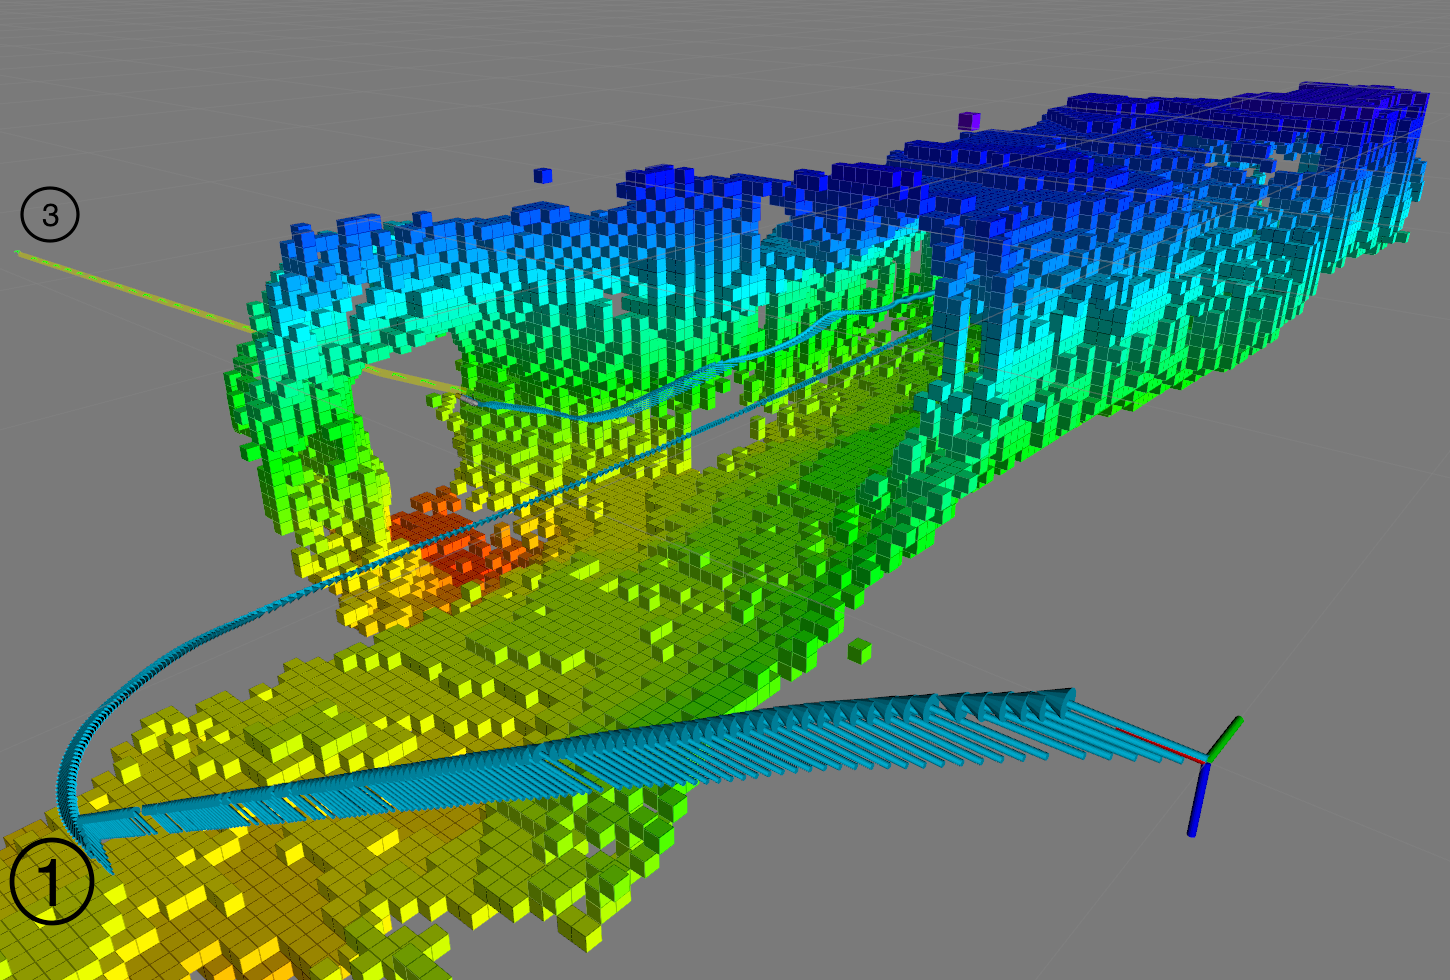
\includegraphics[width=.70\linewidth]{CavesMultS2G_Q3_RViz}}\\
   	\subfloat[Sparus~II traversing the underwater tunnel]{
		\label{fig:CavesMultS2G_Q3_UWSim}
   		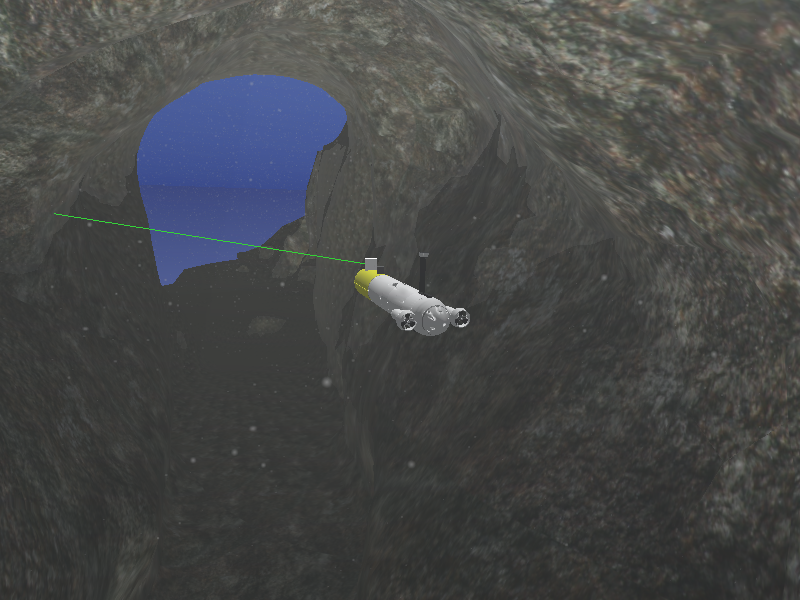
\includegraphics[width=.70\linewidth]{CavesMultS2G_Q3_UWSim}}
\caption[Simulated mission in the caves complex. Third start-to-goal query.]
{Simulated mission in the caves complex. The third start-to-goal query guided
the \ac{AUV} to the second single-branch cave's entrance. In \protect
\subref{fig:CavesMultS2G_Q3_RViz} the vehicle trajectory appears in light blue,
and the remaining of the calculated path in yellow. This query required the
vehicle not only to find a way out of the first cave, but also to traverse a
tunnel that connects the entrances of both single-branch caves.}
\label{fig:CavesMultS2G_Q3}
\end{figure}

Once the Sparus~II \ac{AUV} had crossed the tunnel, the fourth query was defined
to navigate through and until the end of the second single-branch cave, \ie
$q_{goal_4} = [60.0, 87.0, 9.0, 1.82]$. To do so, the speed constrains were kept
as established for the previous query. Once this was accomplished, the fifth
query was set to guide the \ac{AUV} close to a third cave's entrance; this meant
$q_{goal_5} = [82.0, 47.0, 17.0, 0.0]$. This latter query required the planner
to find a way out of the second cave, which is considerably narrower than the
first one. To cope with this latter situation, the planner used a lower surge
speed, $v=0.1m/s$, which allowed the vehicle to turn back with a smaller turning
radius. Figure~\ref{fig:CavesMultS2G_Q4_Q5} depicts part of the execution of
these two queries.

\begin{figure}[htbp]
\myfloatalign
	\subfloat[Sparus~II traversing the second cave]{
		\label{fig:CavesMultS2G_Q4_RViz}
   		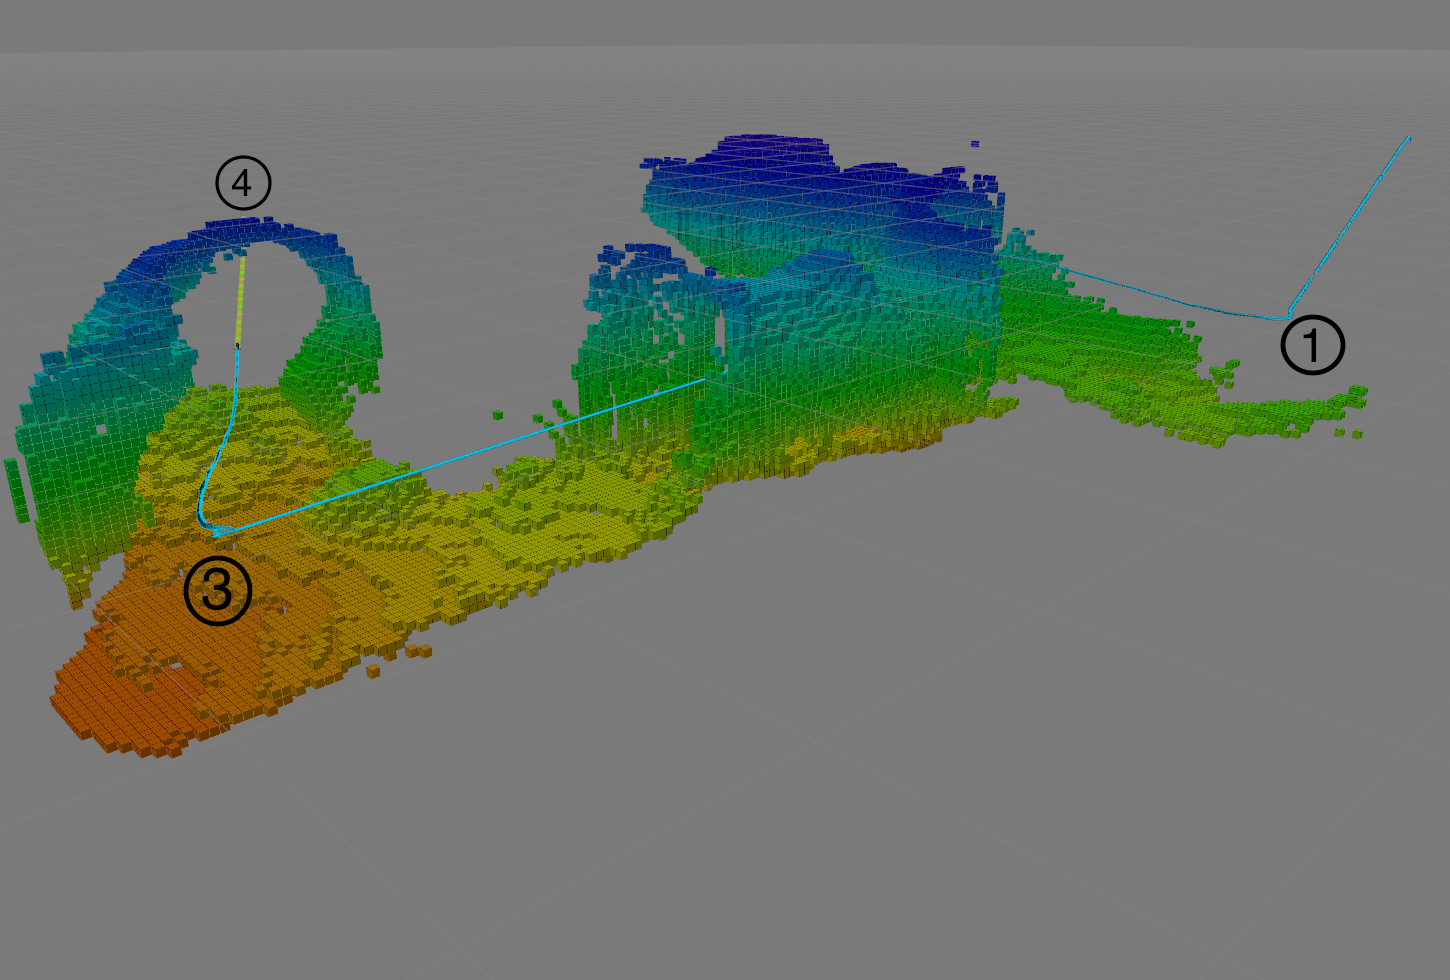
\includegraphics[width=.70\linewidth]{CavesMultS2G_Q4_RViz}}\\
   	\subfloat[Sparus~II on its way back to the third cave's entrance]{
		\label{fig:CavesMultS2G_Q5_RViz}
   		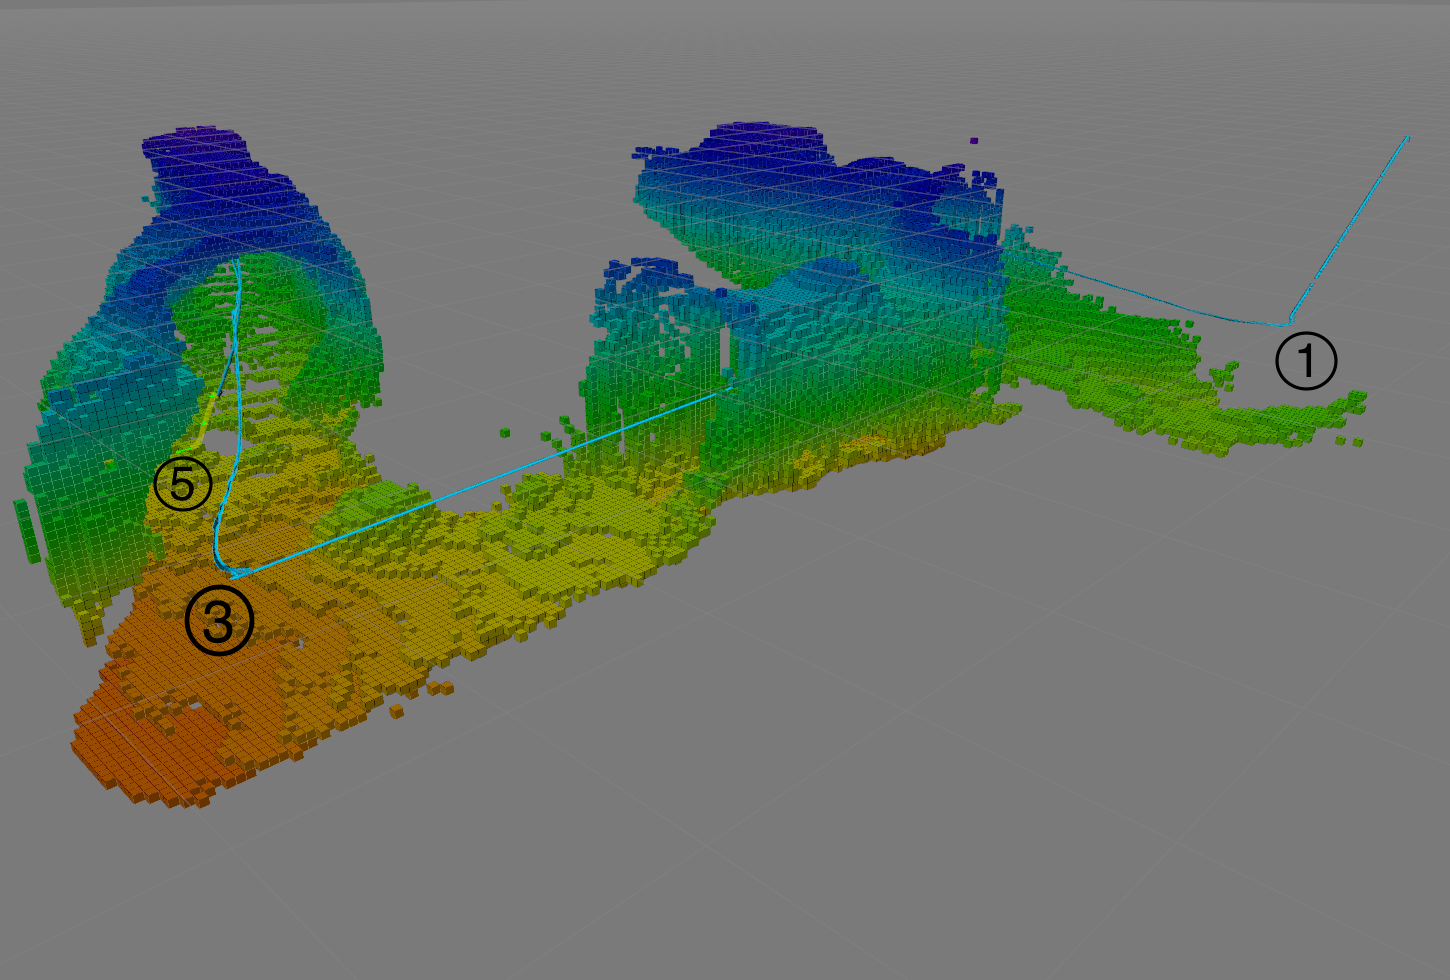
\includegraphics[width=.70\linewidth]{CavesMultS2G_Q5_RViz}}
\caption[Simulated mission in the caves complex. Fourth and fifth start-to-goal
queries.] 
{Simulated mission in the caves complex.
\protect \subref{fig:CavesMultS2G_Q4_RViz} The fourth start-to-goal query
required the vehicle to navigate through the second single-branch cave. 
\protect \subref{fig:CavesMultS2G_Q5_RViz} The fifth query was defined to guide
the vehicle close to a third cave's entrance. This required the planner to find
a way out of the cave. In both images, the vehicle trajectory appears in light
blue, and the remaining of the calculated path in yellow.}
\label{fig:CavesMultS2G_Q4_Q5}
\end{figure}

Finally, Figure~\ref{fig:CavesMultS2G} presents different views of the whole
mission execution, where both the vehicle trajectory and the Octomap built along
the mission can be observed.

% \begin{figure}[htbp]
% \myfloatalign
% 	\subfloat[]{
% 		\label{fig:CavesMultS2G_Q5_RViz}
%    		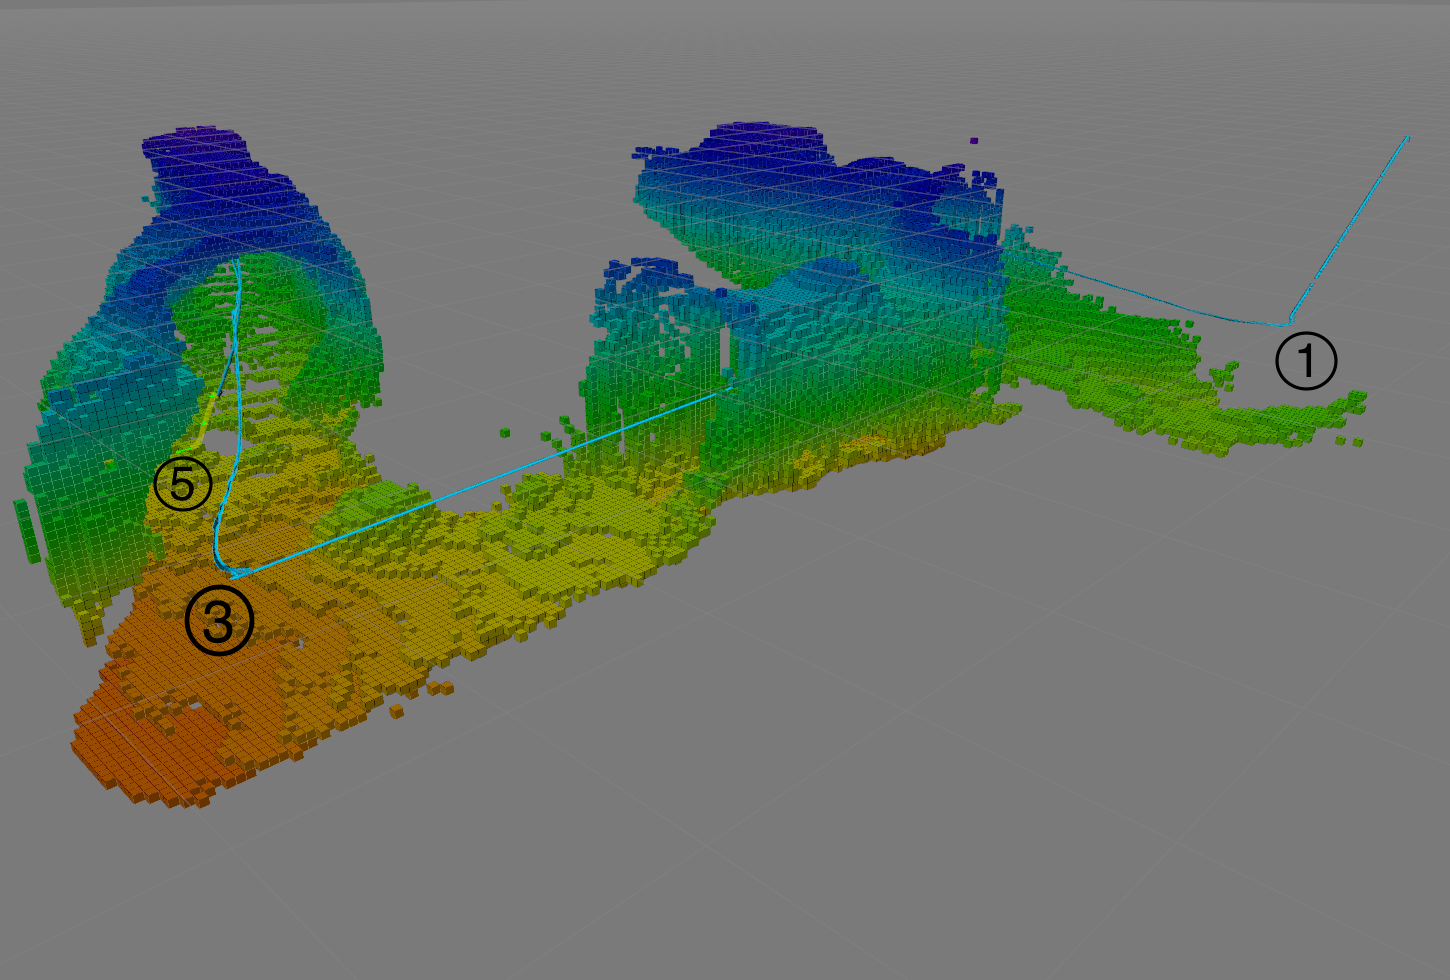
\includegraphics[width=.70\linewidth]{CavesMultS2G_Q5_RViz}}\\
%    	\subfloat[]{
% 		\label{fig:CavesMultS2G_Q5_UWSim}
%    		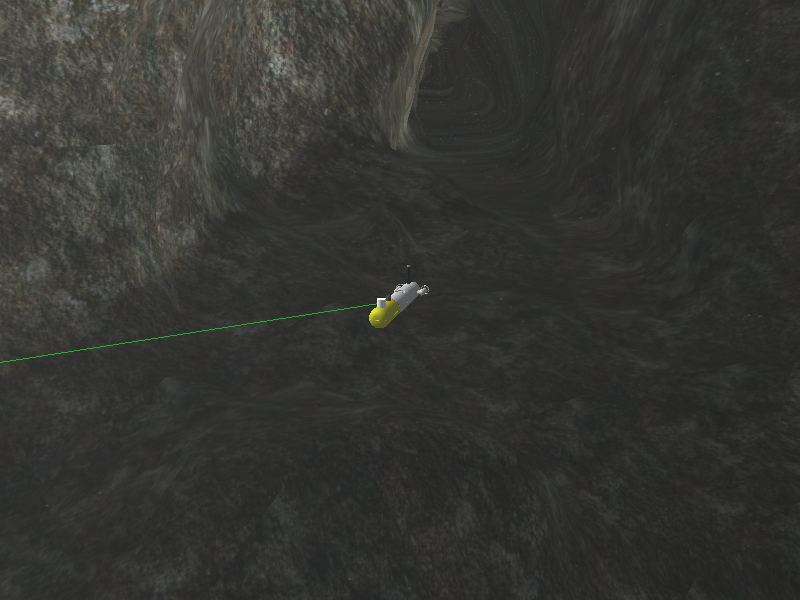
\includegraphics[width=.70\linewidth]{CavesMultS2G_Q5_UWSim}}
% \caption[.]
% {.}
% \label{fig:CavesMultS2G_Q5}
% \end{figure}

% \begin{figure}[htbp]
% 	\myfloatalign
%    	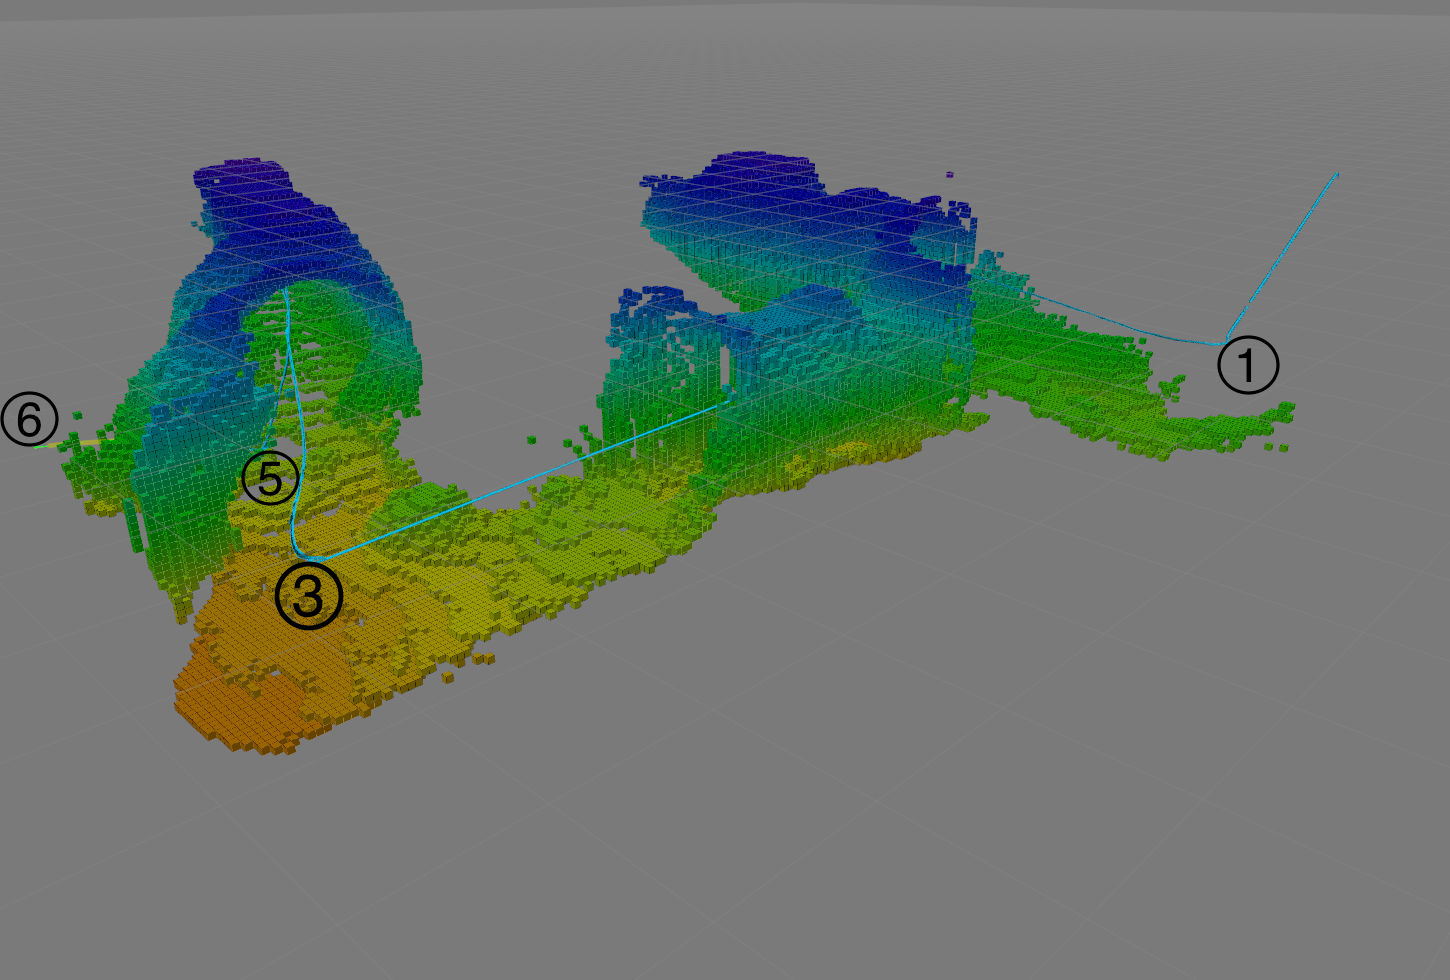
\includegraphics[width=.70\linewidth]{CavesMultS2G_Q6_RViz}
% \caption[.]
% {.}
% \label{fig:CavesMultS2G_Q6}
% \end{figure}

\begin{figure}[htbp]
\myfloatalign
	\subfloat[Top view]{
		\label{fig:CavesMultS2G_TopMap}
   		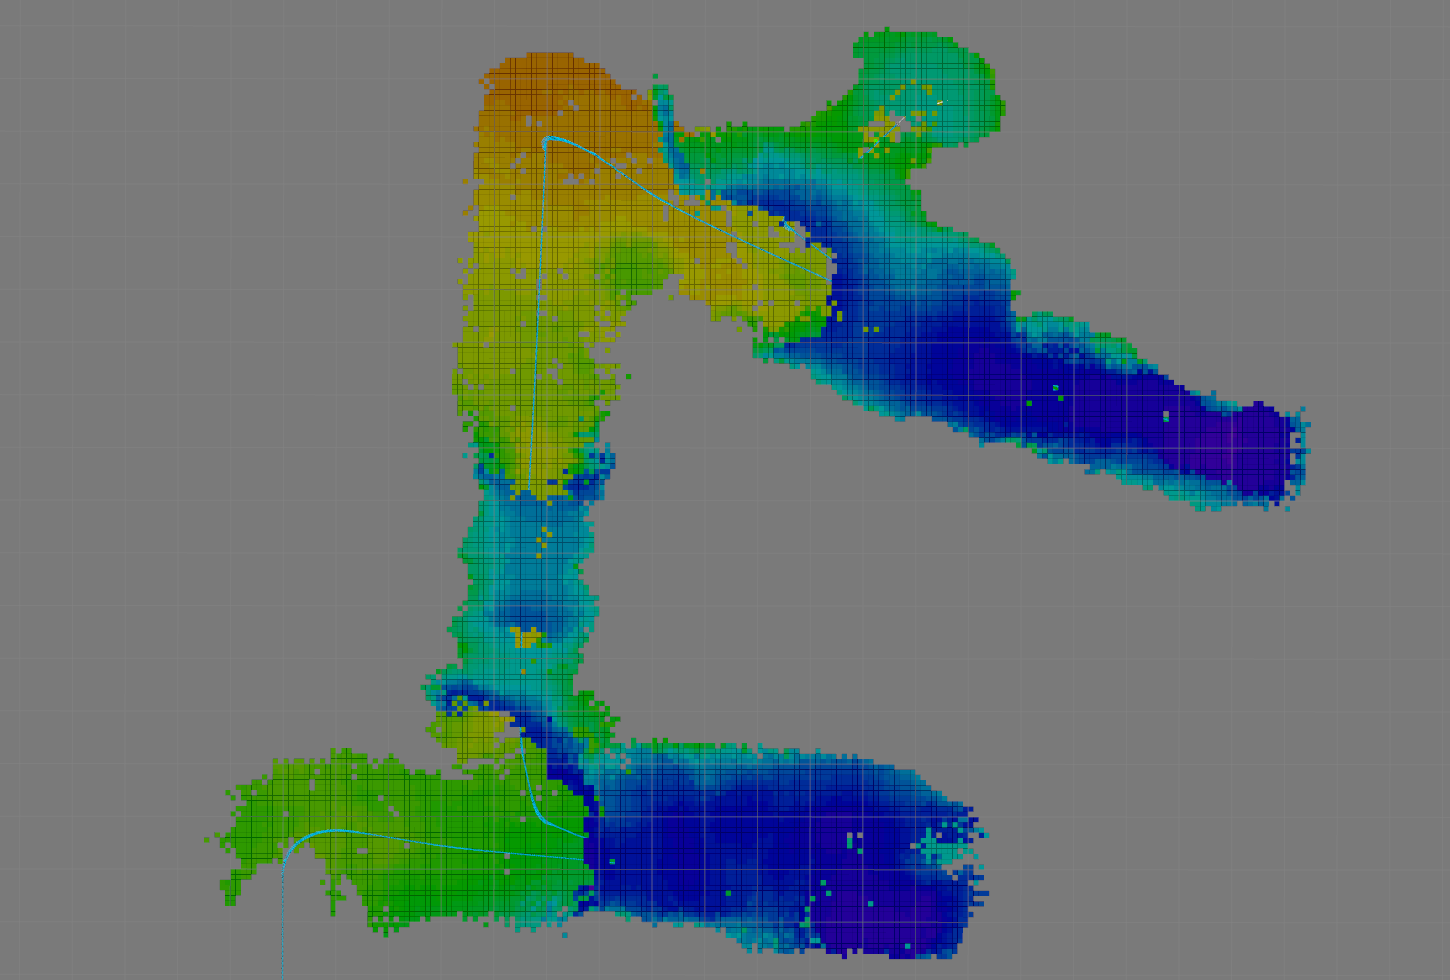
\includegraphics[width=.47\linewidth]{CavesMultS2G_TopMap}}\quad
   	\subfloat[Top view]{
		\label{fig:CavesMultS2G_TopTraj}
   		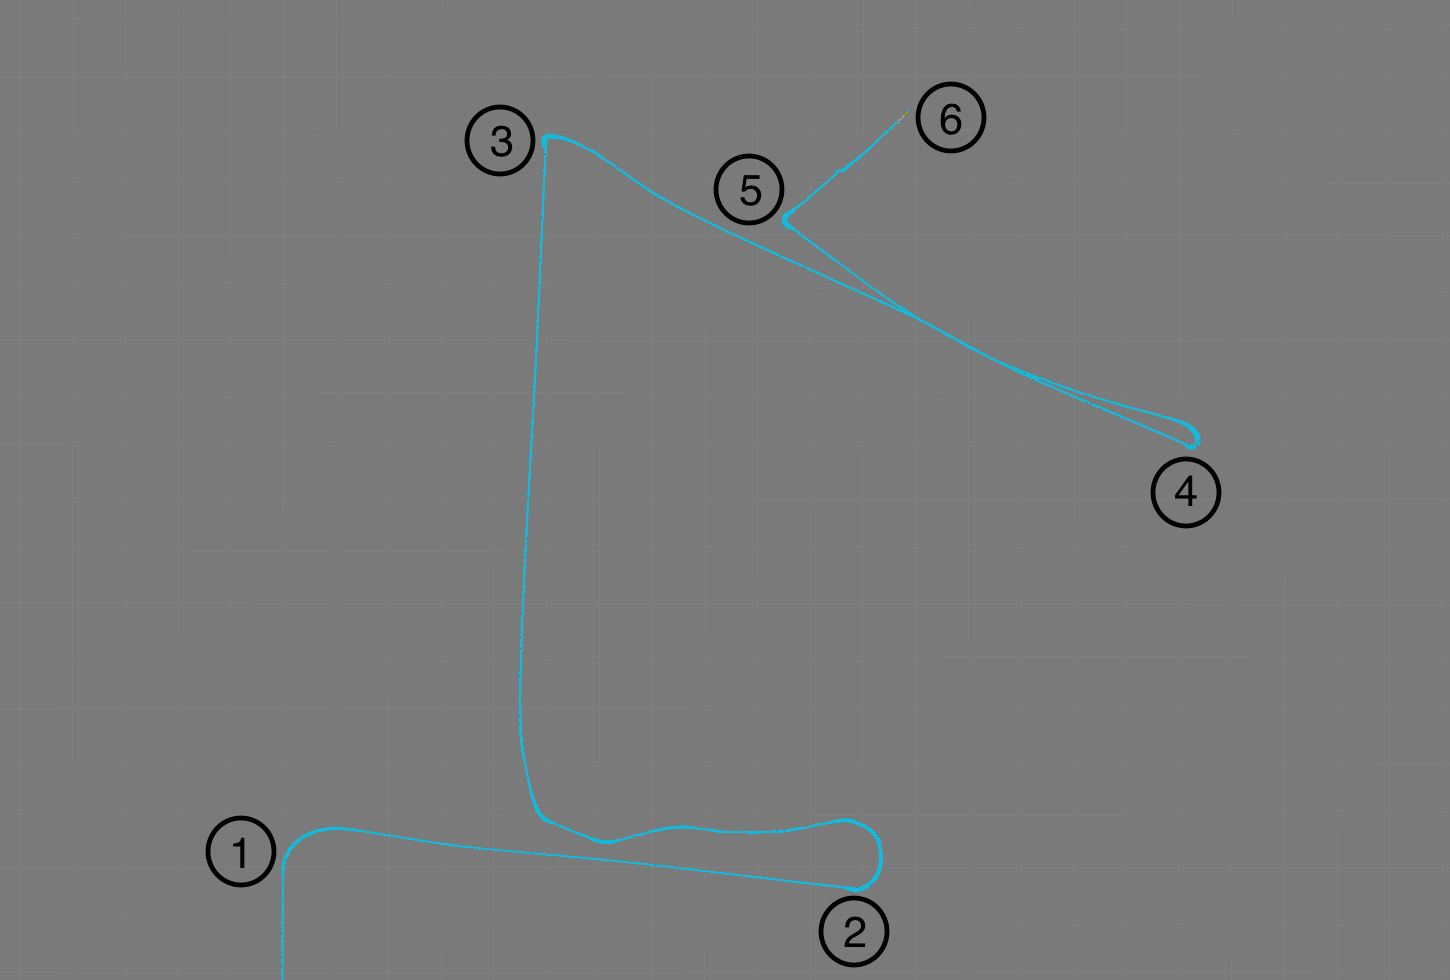
\includegraphics[width=.47\linewidth]{CavesMultS2G_TopTraj}}\\
   	\subfloat[Perspective front view]{
		\label{fig:CavesMultS2G_FrontMap}
   		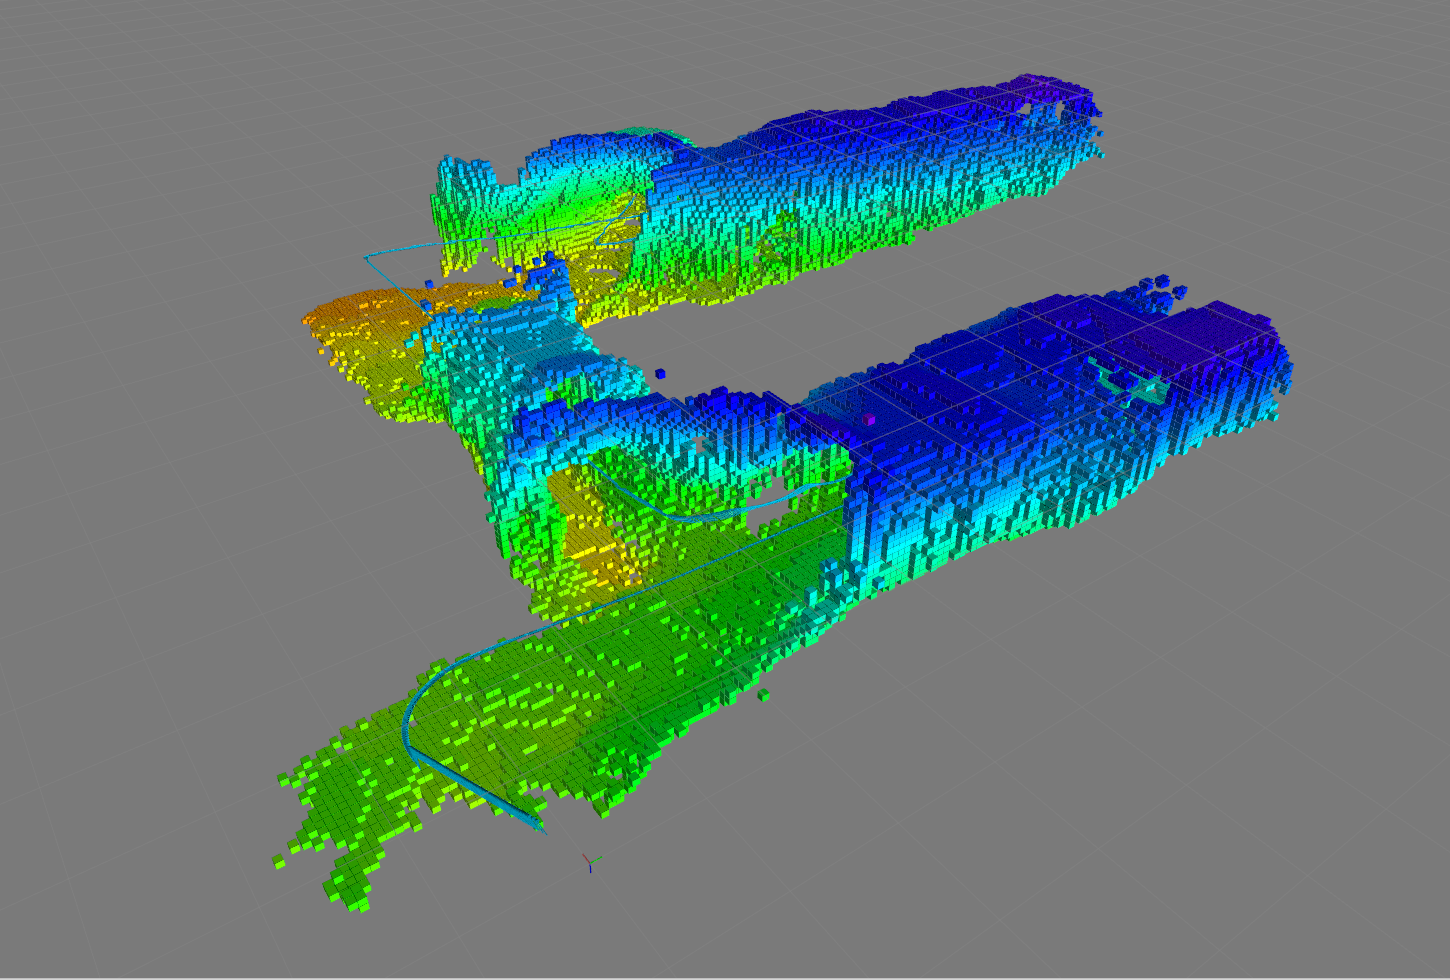
\includegraphics[width=.47\linewidth]{CavesMultS2G_FrontMap}}\quad
   	\subfloat[Perspective front view]{
		\label{fig:CavesMultS2G_FrontTraj}
   		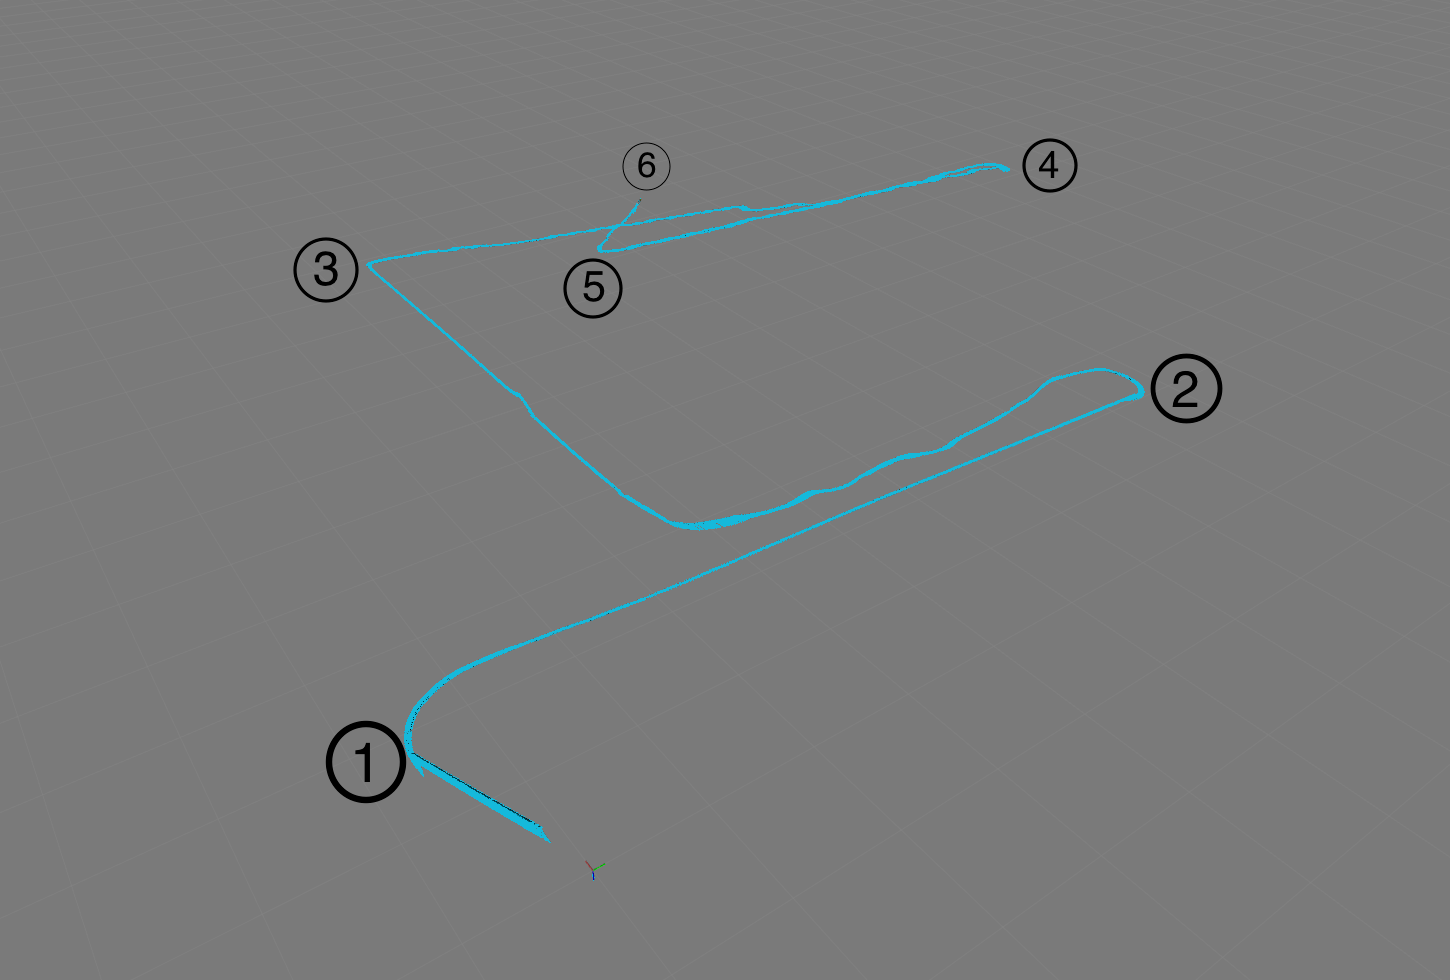
\includegraphics[width=.47\linewidth]{CavesMultS2G_FrontTraj}}\\
   	\subfloat[Perspective back view]{
		\label{fig:CavesMultS2G_BackMap}
   		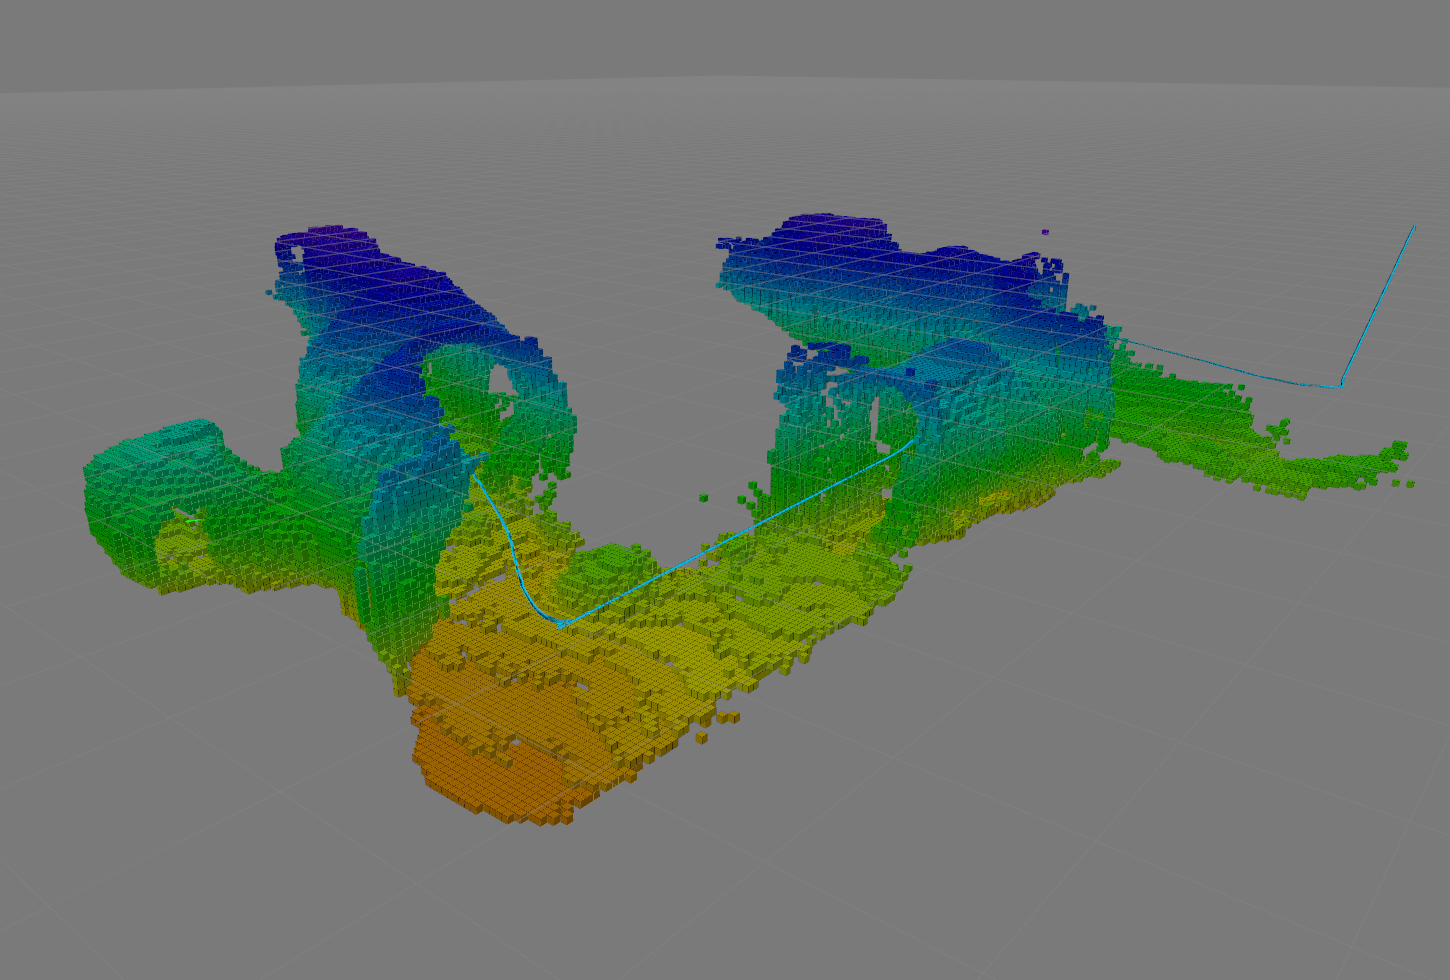
\includegraphics[width=.47\linewidth]{CavesMultS2G_BackMap}}\quad
   	\subfloat[Perspective back view]{
		\label{fig:CavesMultS2G_BackTraj}
   		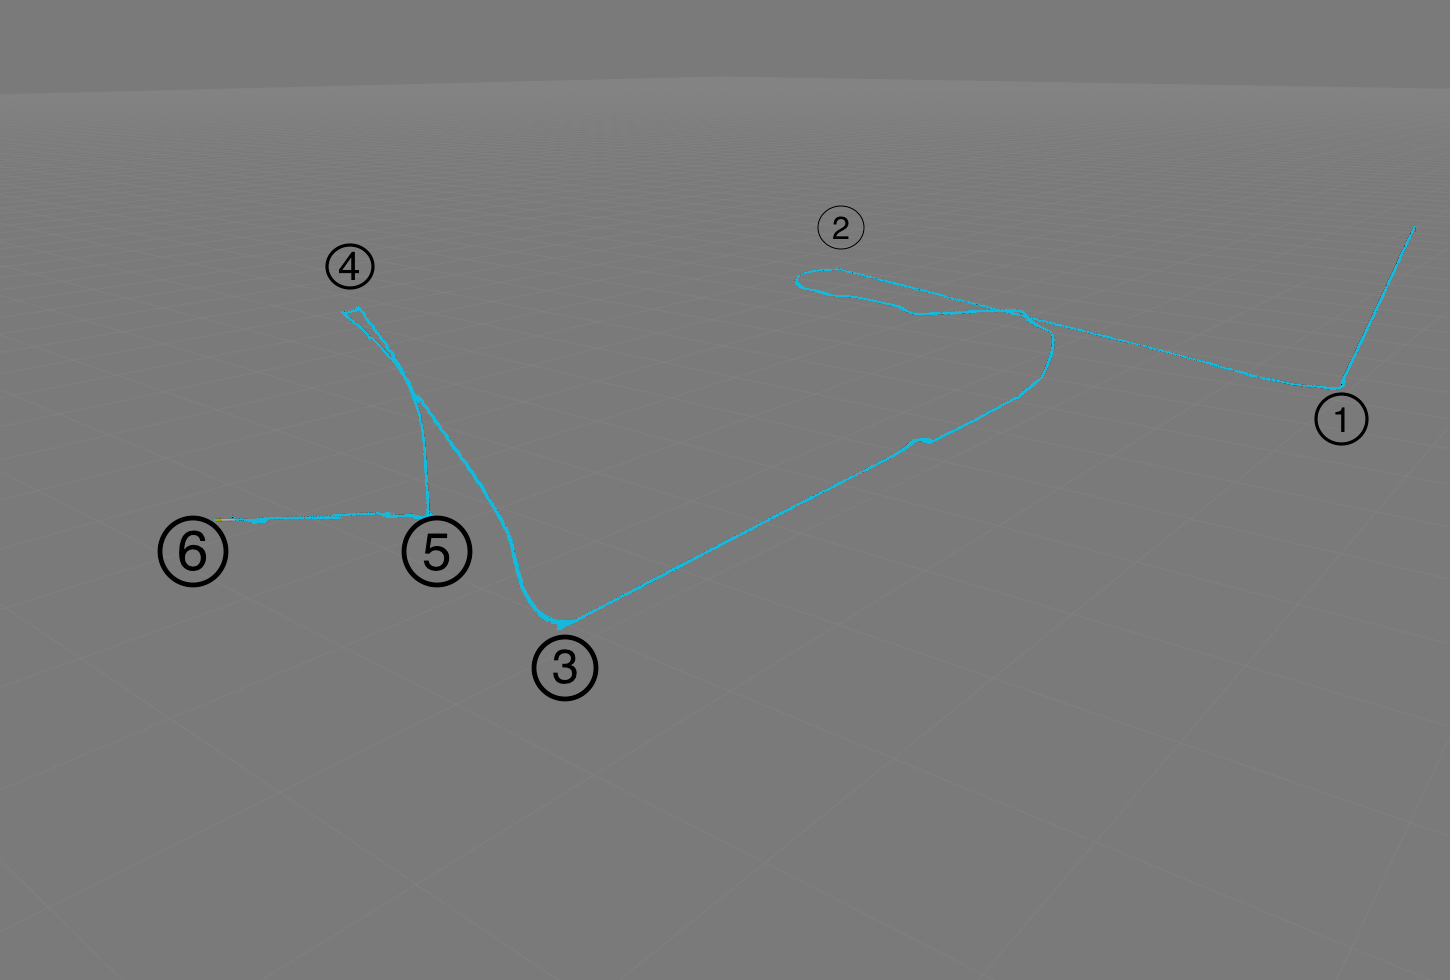
\includegraphics[width=.47\linewidth]{CavesMultS2G_BackTraj}}
\caption[Simulated mission in the caves complex. Whole mission execution.]
{Simulated mission in the caves complex. The whole mission was composed of six
start-to-goal queries that were executed consecutively.}
\label{fig:CavesMultS2G}
\end{figure}

Figure~\ref{fig:CavesMultS2G} presented a mission in an environment that has
been created from a real-world dataset. This test not only evaluates all the
aspects that have been covered throughout this thesis, but also represents a
clear advance towards fully autonomous inspections. However and as it was
mentioned before, there are still some technical aspects that have to be further
developed in order to successfully conduct in-water trials. Some of these
aspects will be analysed and discussed in the next chapter.

\section{Gap Filling and Potential Target Inspection}

The experiments presented in the previous sections have attempted to prove the
capabilities of the proposed path/motion planning framework. But as it was also
mentioned before, in order to make some of these kind of missions a reality,
there are still additional technical aspects that have to be tackled. For this
reason, some of the framework's validation tests have been limited to conduct
simulations over real-world datasets. One example of this is the capability to
plan feasible \ac{3D} paths, which was evaluated with the exploration of
confined natural environments. In order to complement the validation of this
feature, this section presents another experiment that has been carried out with
the AsterX \ac{AUV}.

In most of the current operational and commercial \acp{AUV}, a mission plan is
generally defined in advanced by an operator. Such a mission seeks to cover a
predefined area from a constant and safe altitude. To do so, the mission
commonly consists of the path to be followed and a series of payload commands.
These commands establish when and where sensors must acquire different data
along the specific route. Therefore, the nature of the data mainly depends on
the mission objectives, as well as the sensors installed in the vehicle, \eg
sonars, optical cameras and even physico-chemical sensors.

In this approach of covering a predefined area, the preplanned route is
generally not modified during the survey. Instead, the objective is to sweep the
area in order to detect and localize potential targets, which can include
geological formations~\cite{Galceran2012}, shipwrecks~\cite{Gracias2013}, and
other artificial or natural underwater structures~\cite{Escartin2013}. A common
approach in this kind of missions is to conduct a first exhaustive survey, and
then extract and analyse the gathered data to program a second and more specific
survey. This latter one attempts to obtain more details about the potential
targets, as well as to cover possible gaps resulted during the first
exploration. However, this two-survey strategy can be inefficient, since it
requires establishing a communication link between the \ac{AUV} and its operator
(located in the mother ship) for retrieving the data and reprogramming a new
mission. This is particularly unnecessary in modern \acp{AUV} with long-term
autonomy.

Aiming to overcome some of the aforementioned limitations, one alternative is to
endow an \ac{AUV} with a mission planner, or high-level controller, that extends
its decision-making capabilities. This additional control layer must allow the
vehicle not only to conduct predefined surveys, but also to autonomously detect
and inspect potential subareas of interest without the need of resurfacing. To
do so, the \ac{AUV} is assumed to be equipped with a looking-downward
multibeam sonar, which gathers data from the sea bottom along the initial
mission. This data can be then automatically processed onboard in order to
detect anomalies and gaps, which are marked as regions that require further
inspection, thus enlarging the original survey. In the case of anomalies (\ie
objects that protrude above the surrounding seafloor), the vehicle must conduct
closer explorations; while in the case of gaps, it must complete covering the
area that was initially defined.

To implement this approach over a particular \ac{AUV}, it is necessary to first
understand its control architecture. In what concerns the AsterX, it is composed
of three main functional blocks (see Appendix~\ref{appx:exp_platform},
Fig.~\ref{fig:HighLevelControArch}): 1) the low-level controller, or
\textit{frontseat}, which runs over QNX; 2) the high-level controller, or
\textit{backseat}, which runs over \acf{ROS}; and 3) the \textit{payload}
controller\footnote{For more details, the interest readers are encouraged to
look into Appendix~\ref{appx:exp_platform}}. Having this in mind, the proposed
mission planner can be developed within the \textit{backseat}, which allows
including different specialized processes, or nodes as referred to in
\ac{ROS}. Figure~\ref{fig:BackseatDiagram} depicts the \textit{backseat}
controller together with the required nodes. It is also important to notice that
these nodes not only are capable of exchanging information between each other,
but also can externally communicate with the \textit{frontseat} and payload
controllers.

The first of these nodes is called the \textit{target/gap detector}, and it uses
the multibeam data gathered along the initial survey to detect targets
(anomalies) and gaps. The second and central node is called \textit{mission
handler}, and it receives a list of the targets and gaps' positions. Around
these positions, this node establishes subareas of interest. The third node is
the \textit{path planner}, and it is based on the \textit{planning} module
presented in Chapter~\ref{ch:plann_online}. This node calculates \ac{3D}
feasible paths to approach and conduct further exploration or coverage of the
subareas of interest. Finally, once the planner has provided the paths, the
\textit{mission handler} send them to the \textit{path-tracking controller}.
This latter node generates the corresponding \textit{frontseat} controller
setpoints.

\begin{figure}[htbp] %  figure placement: here, top, bottom, or page
\centering
	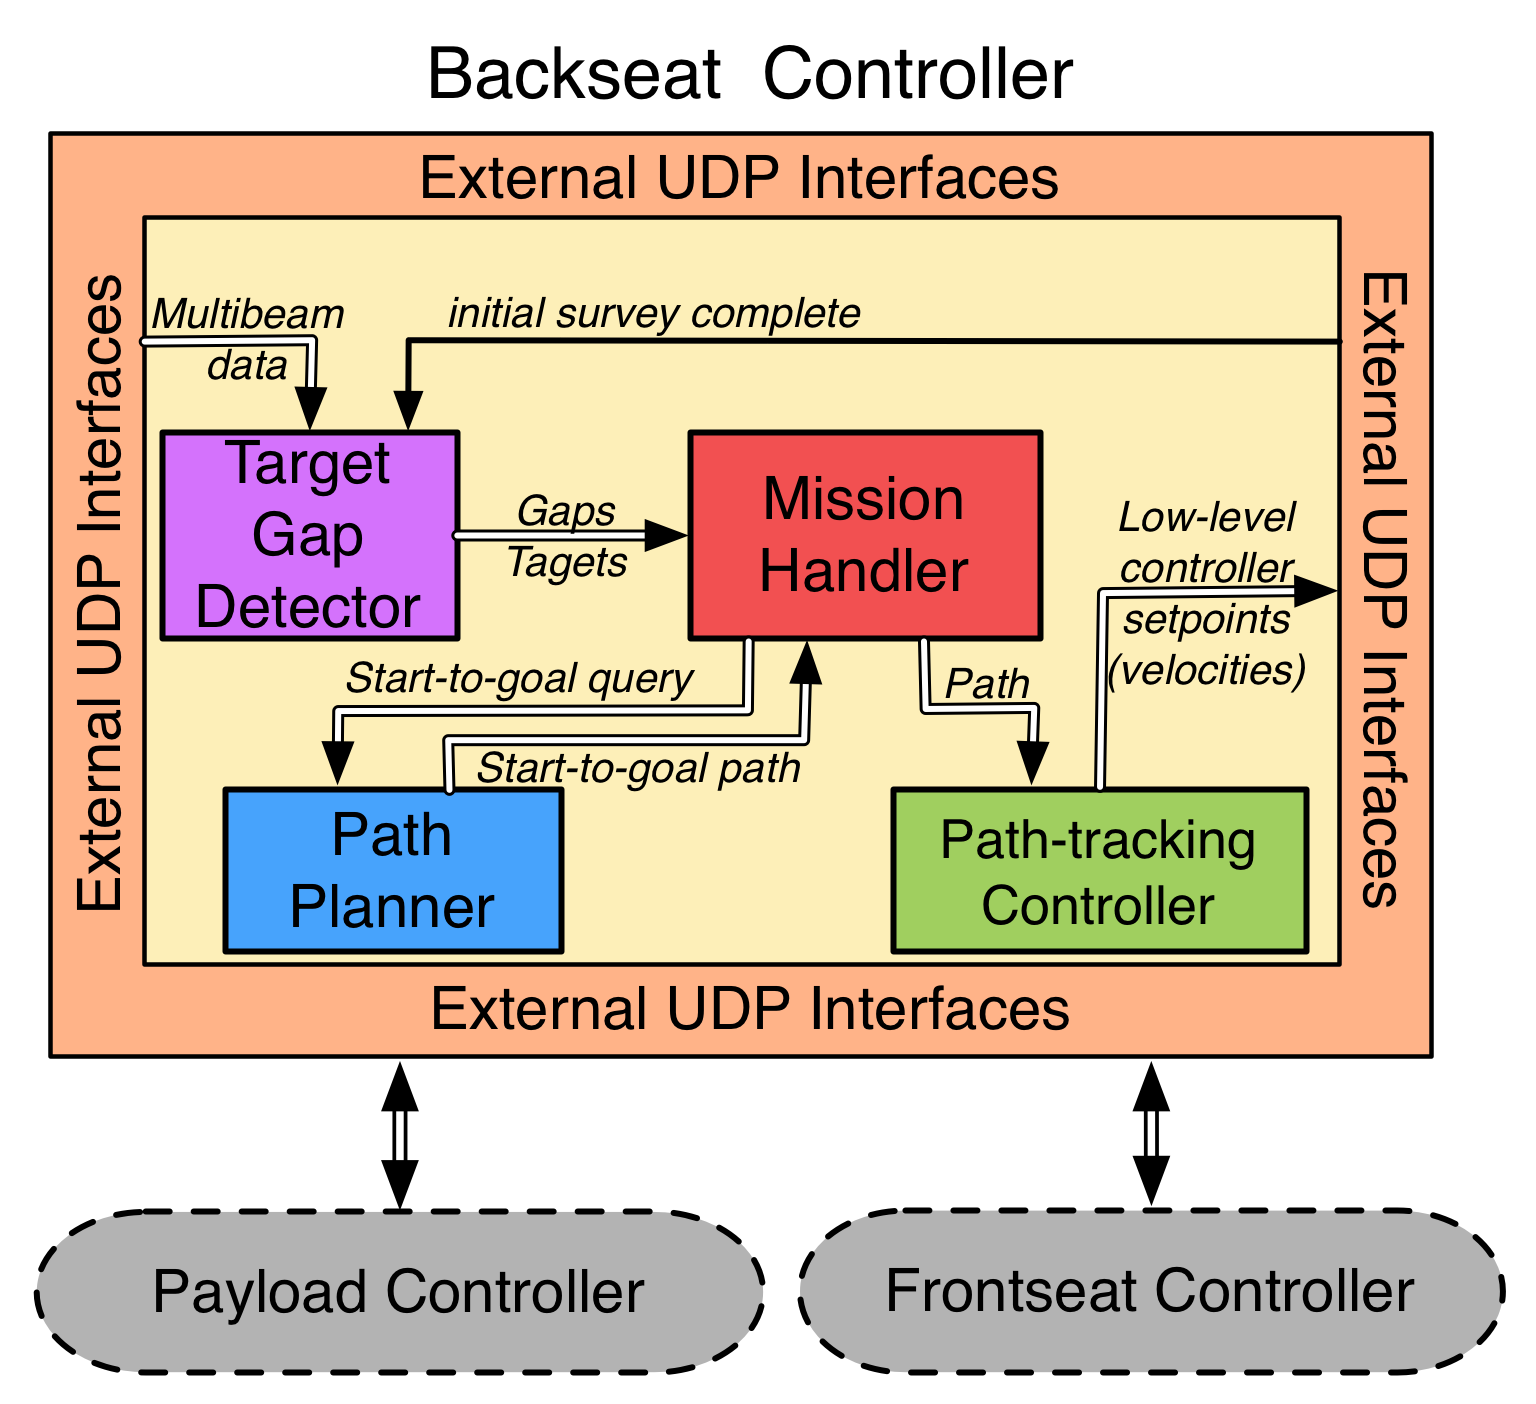
\includegraphics[width=.7\linewidth]{BackseatDiagram}
\caption[Main modules of the \textit{backseat} controller.]
{Main modules of the \textit{backseat} controller}
\label{fig:BackseatDiagram}
\end{figure}

An important aspect of the \textit{path planner} used for this experiment is
the necessity to take into account the vehicle motion constraints involved.
Apart from those constraints associated with a torpedo-shaped \ac{AUV}, the
AsterX can also be limited to navigate at a constant surge speed. This leaves the
turning rate as the variable that determines the \ac{AUV} turning radius.
This formulation coincides with the approach presented in the
Chapter~\ref{ch:motion_constratins}, thus allowing the use of the
\textit{planning} module presented in Chapter~\ref{ch:plann_online}. In order to
validate this new one-survey approach, the AsterX \ac{AUV} conducted a
real-world inspection by using its \textit{backseat} controller with the
functional nodes mentioned before. Figure~\ref{fig:AsterXDeployment} depicts
the deployment of the \ac{AUV} before starting the mission.

\begin{figure}[htbp]
\myfloatalign
	\subfloat[]{
		\label{fig:AsterXDeployment1}
   		\includegraphics[width=.45\linewidth]{AsterXDeployment1}}\quad
   	\subfloat[]{
		\label{fig:AsterXDeployment2}
   		\includegraphics[width=.45\linewidth]{AsterXDeployment2}}\\
   	\subfloat[]{
		\label{fig:AsterXDeployment3}
   		\includegraphics[width=.45\linewidth]{AsterXDeployment3}}
\caption[AsterX AUV deployment from its mother ship.]
{AsterX AUV deployment from its mother ship L'Europe}
\label{fig:AsterXDeployment}
\end{figure}

The mission consisted in detecting and navigating in close proximity to a plane
wreck that is located in the bay of La Ciotat, France. Although the approximate
location was known, it was not considered accurate enough to send the vehicle
closer. Before starting the mission, the AsterX was programmed to follow a
predefined coverage survey of the area of interest. To do so, the \ac{AUV}
navigated at $10m$ deep and with a constant surge speed of $1.5m/s$.
This initial survey was defined within the \textit{frontseat} controller, which,
once completed this first part, handed over the control of the \ac{AUV} to the
\textit{backseat}. Once the \textit{backseat} was informed, it guided the
vehicle over a straight line trajectory while keeping the same speed and safe
altitude. This maneuver was conducted while the \textit{target/gap detector}
processed the multibeam data to detect the potential targets and gaps, if any of
them exist. Figure~\ref{fig:AsterXMission1} depicts the area of interest, the
initial survey, and the potential target and gaps detected from the multibeam
data.


\begin{figure}[htbp] %  figure placement: here, top, bottom, or page
\centering
	\includegraphics[width=.7\linewidth]{AsterXMission1_}
\caption[Potential target and gaps detected after completing the
initial survey with the AsterX AUV.]
{Potential target and gaps detected after completing the initial survey with the
AsterX AUV. It can be observed the area of interest in black, the AUV trajectory
in green, the area covered with multibeam sonar with light grey, and two gaps
and one potential target in white.}
\label{fig:AsterXMission1}
\end{figure}

After the \textit{detector} provided the locations of the potential targets and
gaps, the \textit{path planner} calculated a complementary \ac{3D} trajectory to
both explore the potential targets and cover the gaps. For the former case, the
planner calculated a path $15m$ over than highest point detected in the
target. For the latter case, the planner defined paths to cover the gaps at the
deep of the initial survey, \ie $10m$ for this particular mission. As the
extended mission required navigating at different altitudes, the \textit{planner}
calculated \ac{3D} paths that met the ascending and descending motion
constraints, as it was explained in Chapter~\ref{ch:planning_3D}. Once this
calculation was complete, the whole path was sent to \textit{path-tracking
controller}. Figure~\ref{fig:AsterXMission2} depicts the extended mission to
navigate over the potential target and to cover the gaps.

\begin{figure}[htbp] %  figure placement: here, top, bottom, or page
\centering
	\includegraphics[width=.7\linewidth]{AsterXMission2_}
\caption[Path planned to further cover the potential target and gaps with the
AsterX AUV.] 
{Path planned to further cover the potential target and gaps with the
AsterX AUV. It can be observed the new extended mission in yellow. Although the
view is from the top, the path is 3D since it requires different altitudes to
inspect targets and to cover gaps.}
\label{fig:AsterXMission2}
\end{figure}

As mentioned in the beginning of this section, this experiment allows further
proving the capability of planning \ac{3D} \ac{AUV} paths by using the approach
proposed in this thesis. Figure~\ref{fig:AsterXMission3} depicts how the AsterX
\ac{AUV} further inspected the target by following a calculated path. To do so,
the vehicle descended to a specify altitude with respect to the detected anomaly
(target), while conducting turning maneuvers. Both horizontal and vertical
motions met the vehicle motion capabilities. Finally,
Figure~\ref{fig:AsterXMission4} shows the final \ac{AUV} trajectory after
completing the whole mission. It can be observed how the vehicle not only
traveled over the target, but also covered the gaps.

\begin{figure}[htbp] %  figure placement: here, top, bottom, or page
\centering
	\includegraphics[width=.7\linewidth]{AsterXMission3_}
\caption[The AsterX AUV approaches to further inspect a potential target.]
{The AsterX AUV approaches to further inspect a potential target. The vehicle
trajectory is presented in green, while the calculated path appears in yellow.}
\label{fig:AsterXMission3}
\end{figure}

\begin{figure}[htbp] %  figure placement: here, top, bottom, or page
\centering
	\includegraphics[width=.7\linewidth]{AsterXMission4_}
\caption[The AsterX AUV completed the mission by inspecting the potential
target and covering the gaps from the initial survey.] 
{The AsterX AUV completed the mission by inspecting the potential
target and covering the gaps from the initial survey. It can be observed the
area of interest in black, the AUV trajectory in green, the area covered with
multibeam sonar with light grey.}
\label{fig:AsterXMission4}
\end{figure}

% ---------------------------------------------------------------------------
%: ----------------------- end of thesis sub-document ------------------------
% ---------------------------------------------------------------------------

